\chapter{Appendix}

\section{Application screenshots}

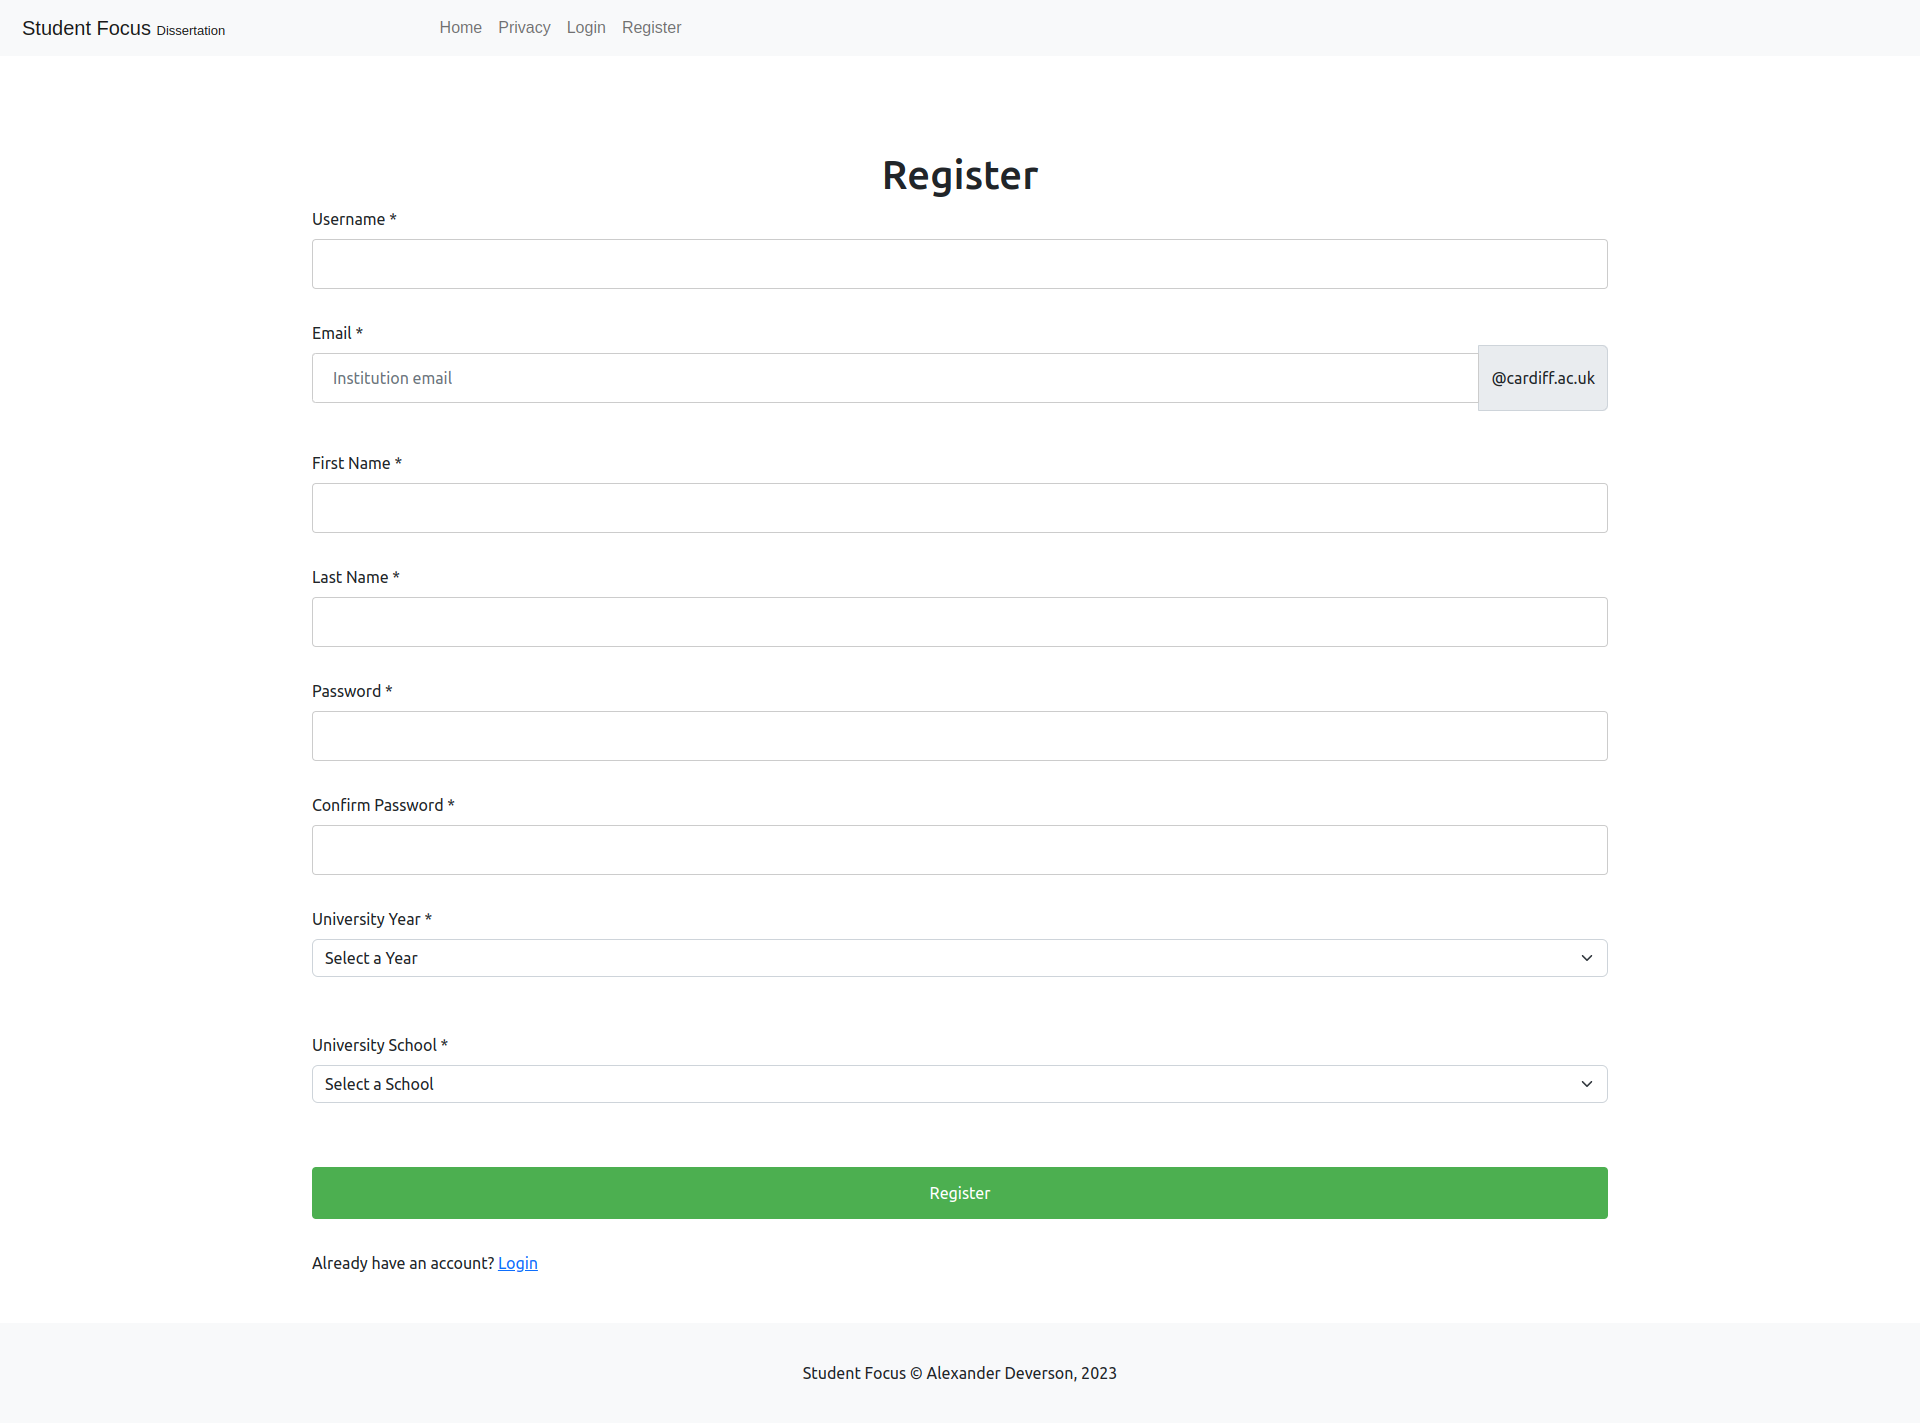
\includegraphics[scale=0.20]{images/application/1 - register.png}

Registration page

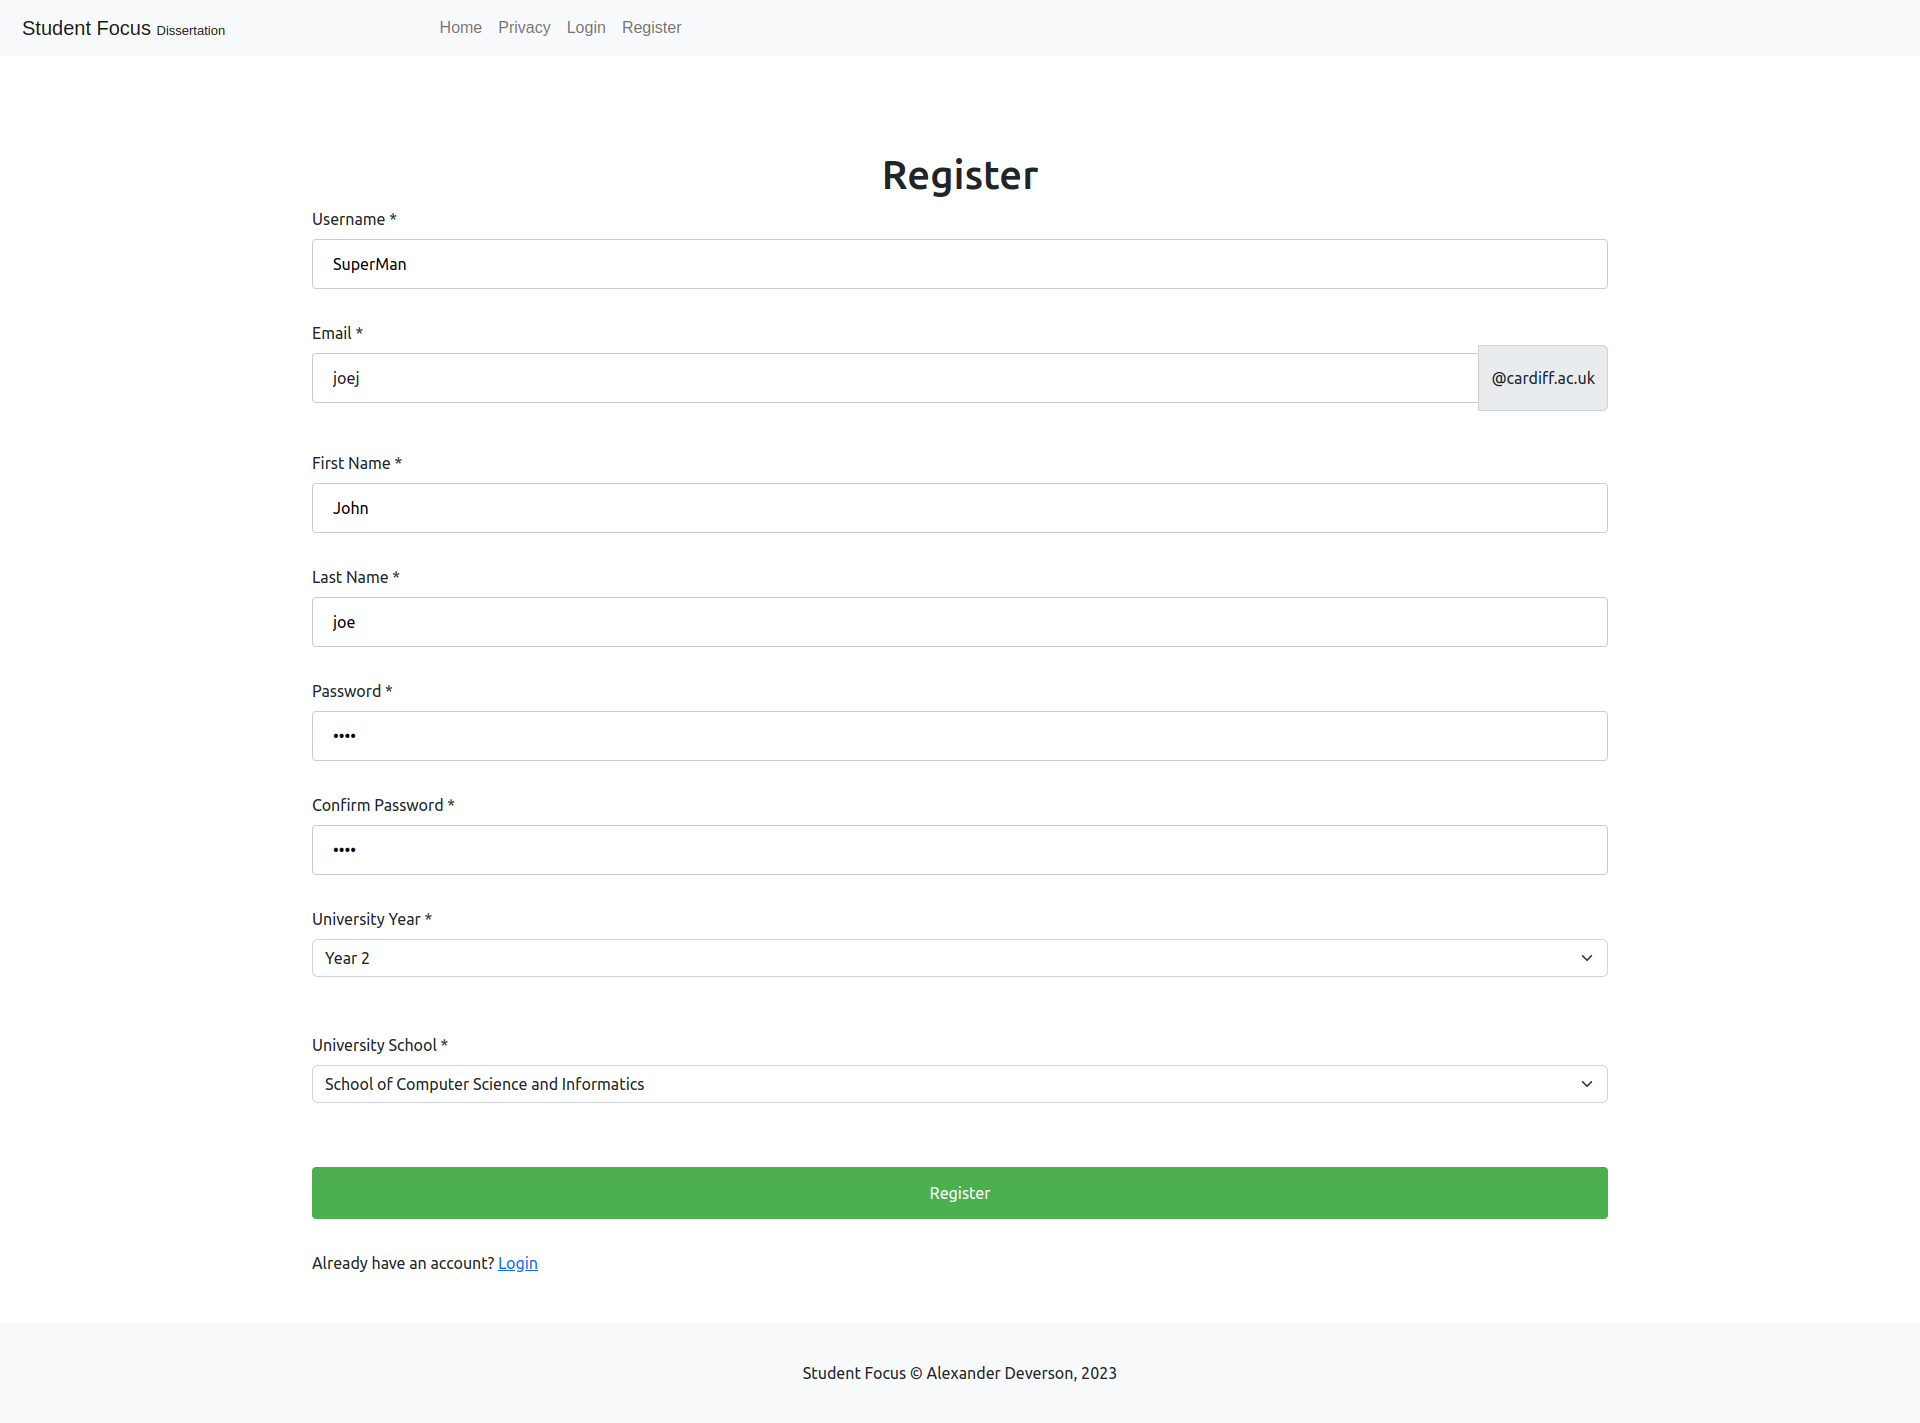
\includegraphics[scale=0.20]{images/application/2 - register_filed_in.png}

Registration page example filled in

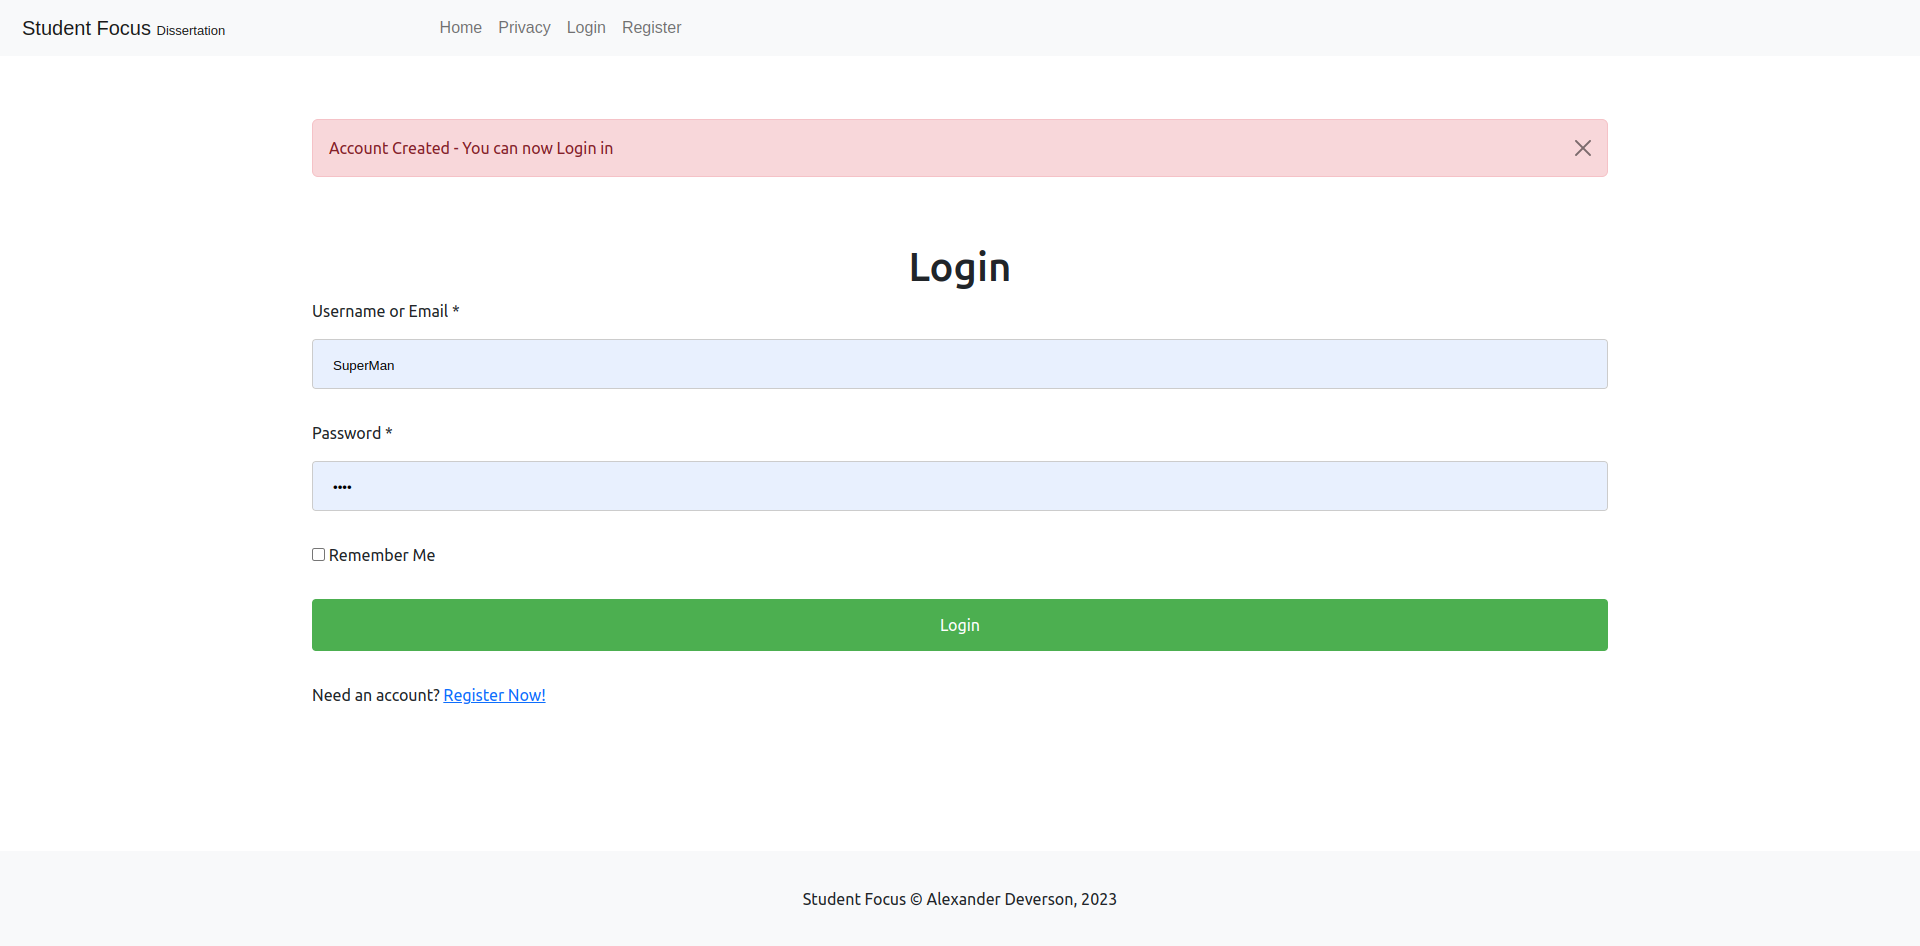
\includegraphics[scale=0.20]{images/application/3 - login_after_reg.png}

Login page

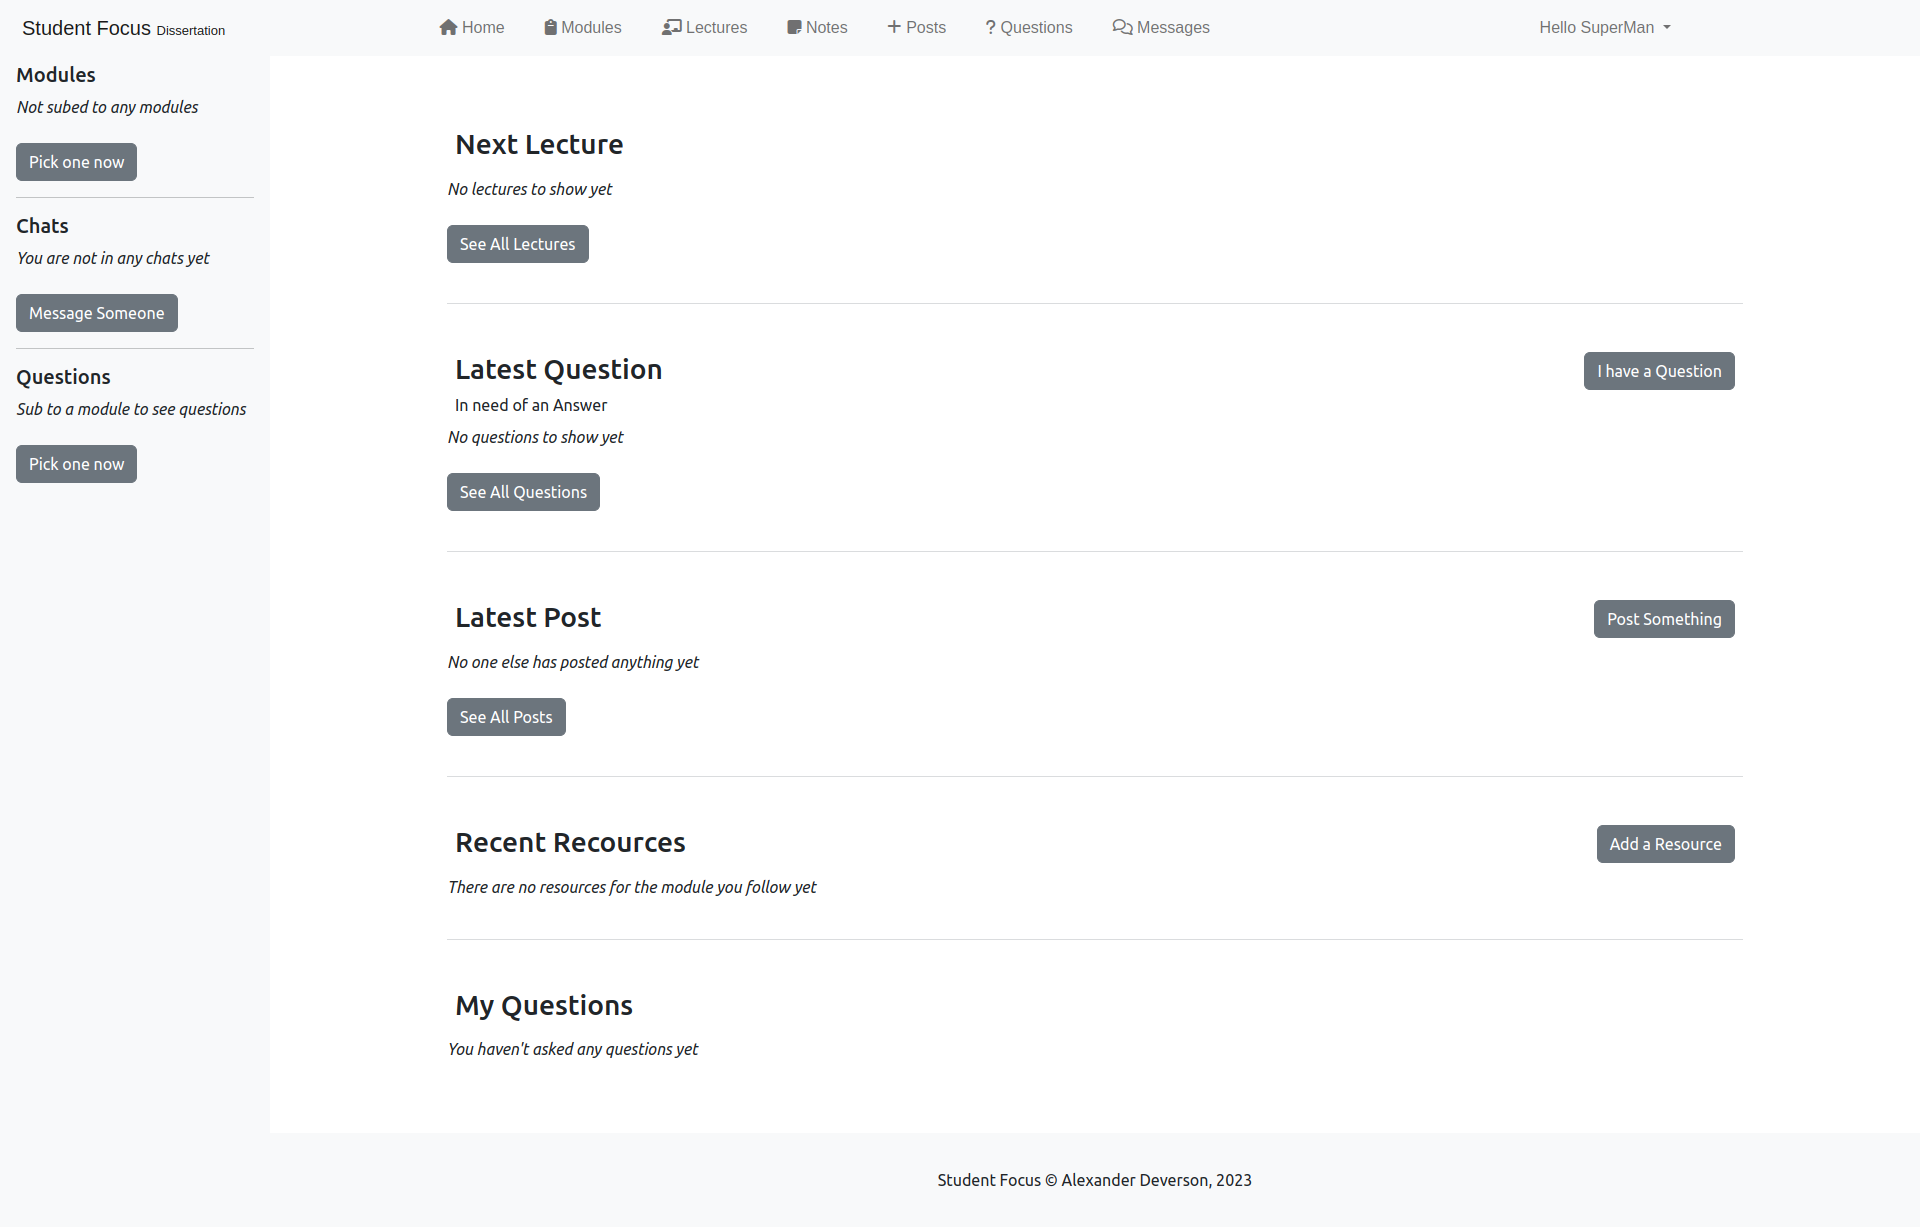
\includegraphics[scale=0.20]{images/application/4 - home_empty.png}

User home page

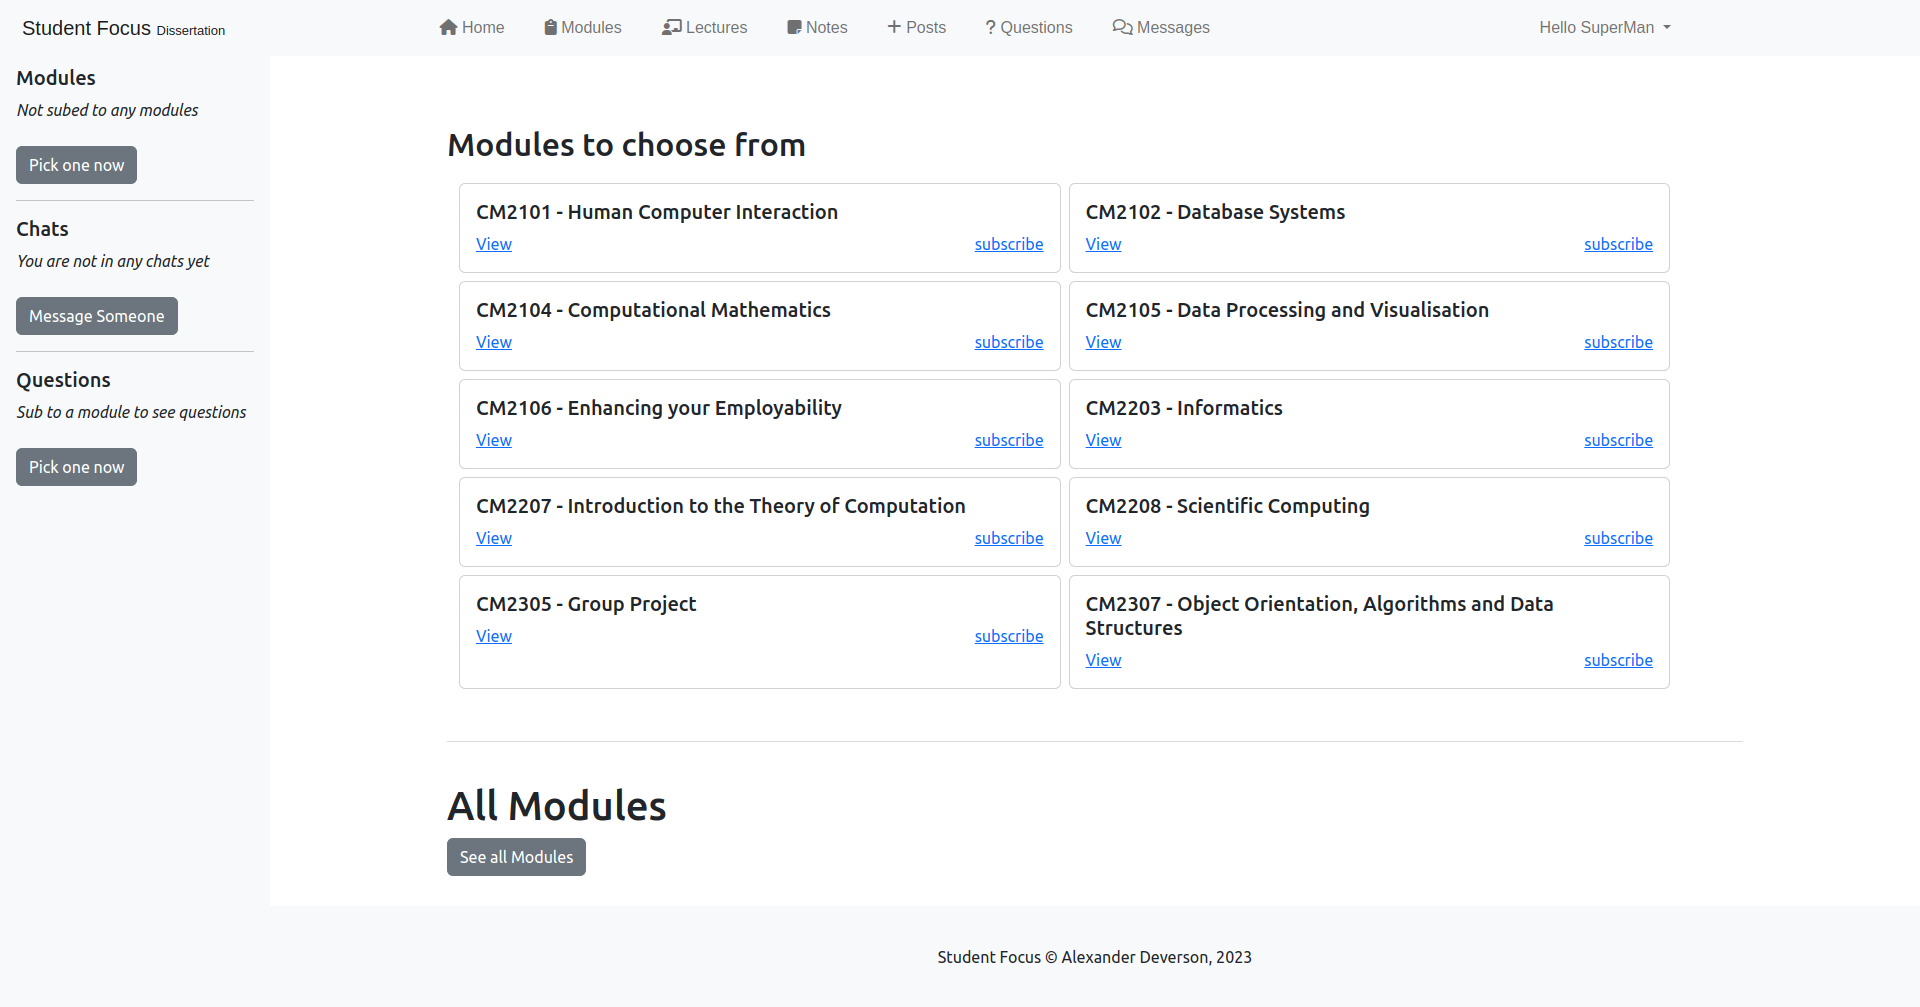
\includegraphics[scale=0.20]{images/application/5 - module_selection.png}

Module selection page

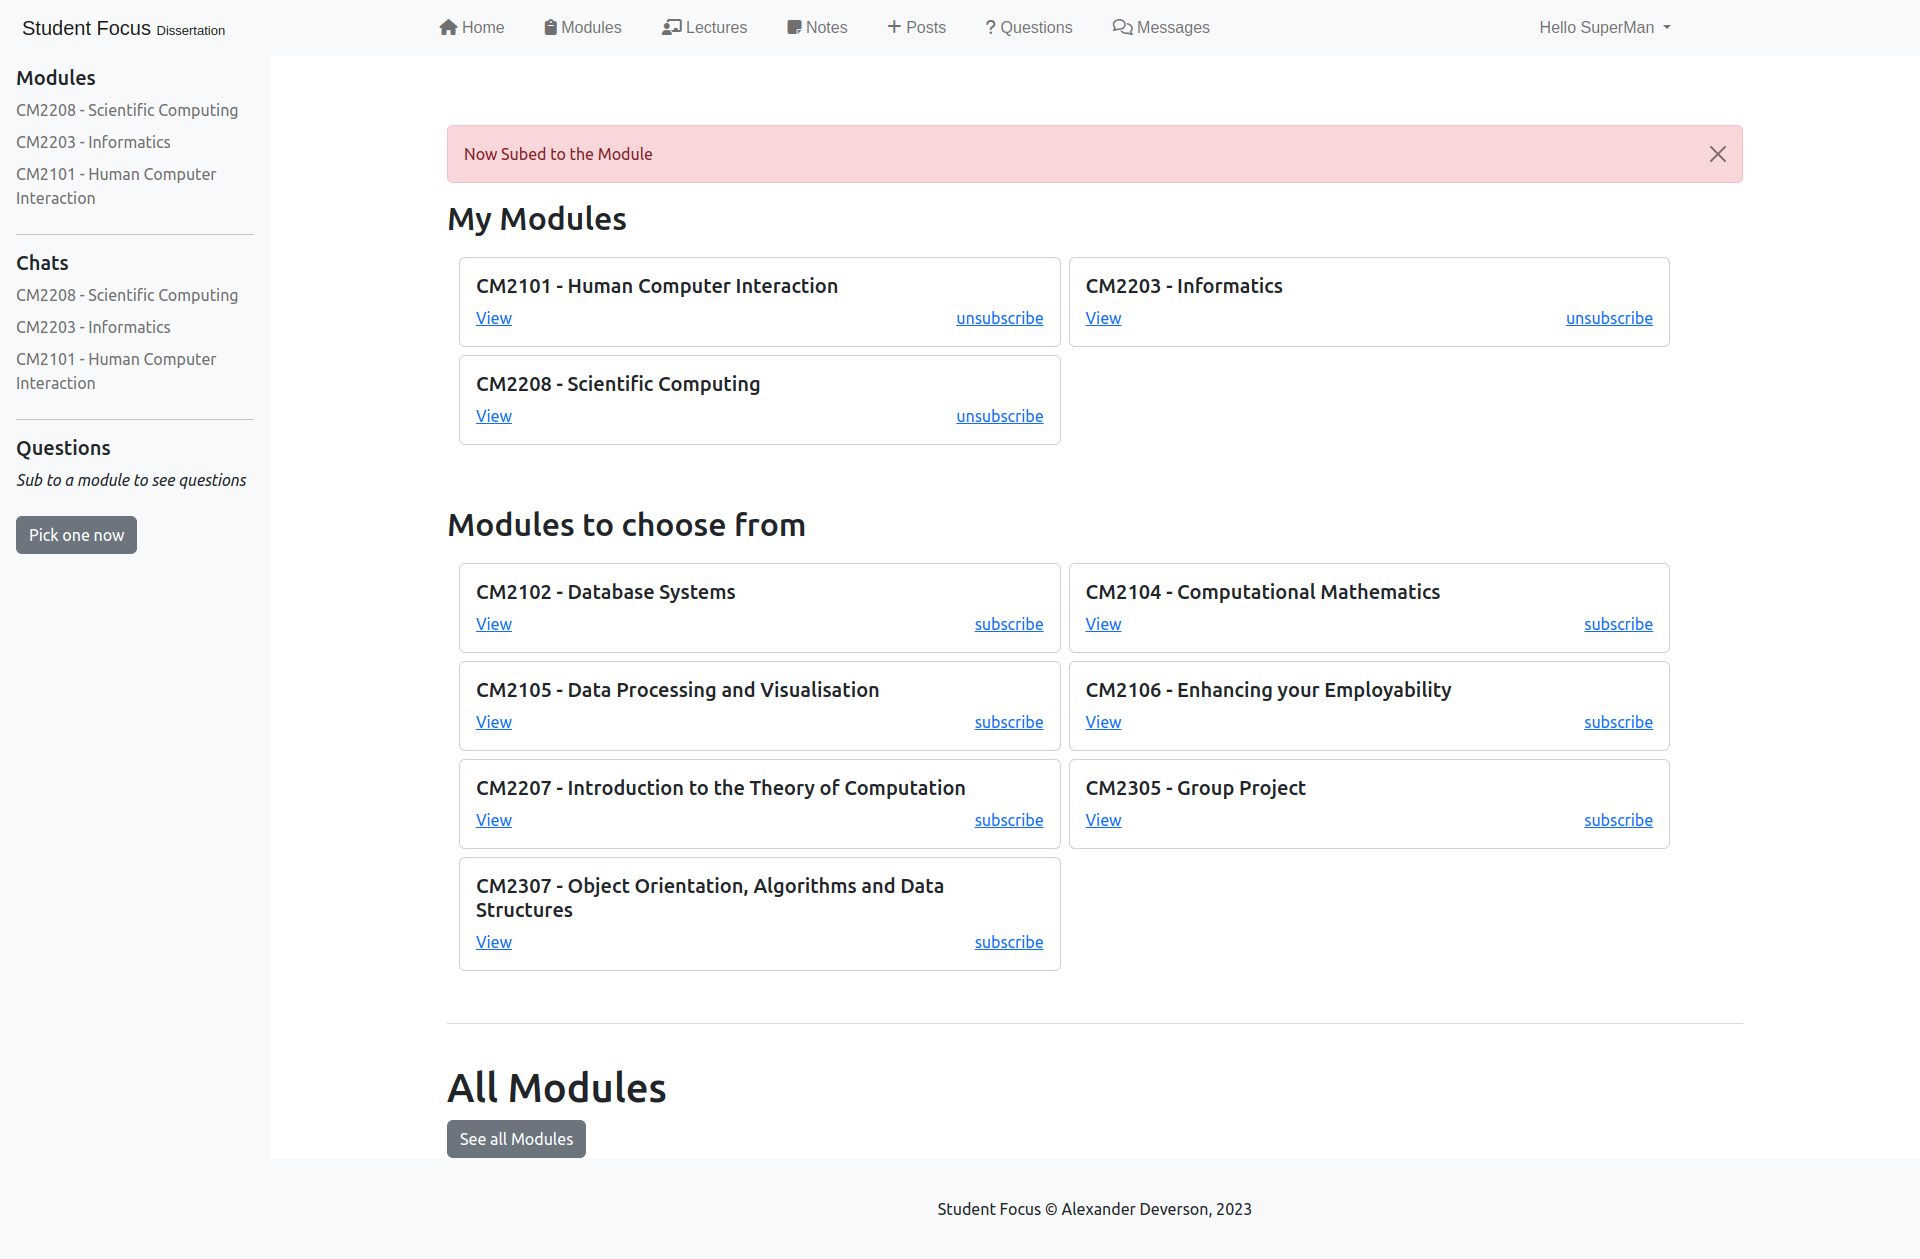
\includegraphics[scale=0.20]{images/application/6 - module_selection_subed.png}

Module selection page after the user subscribes

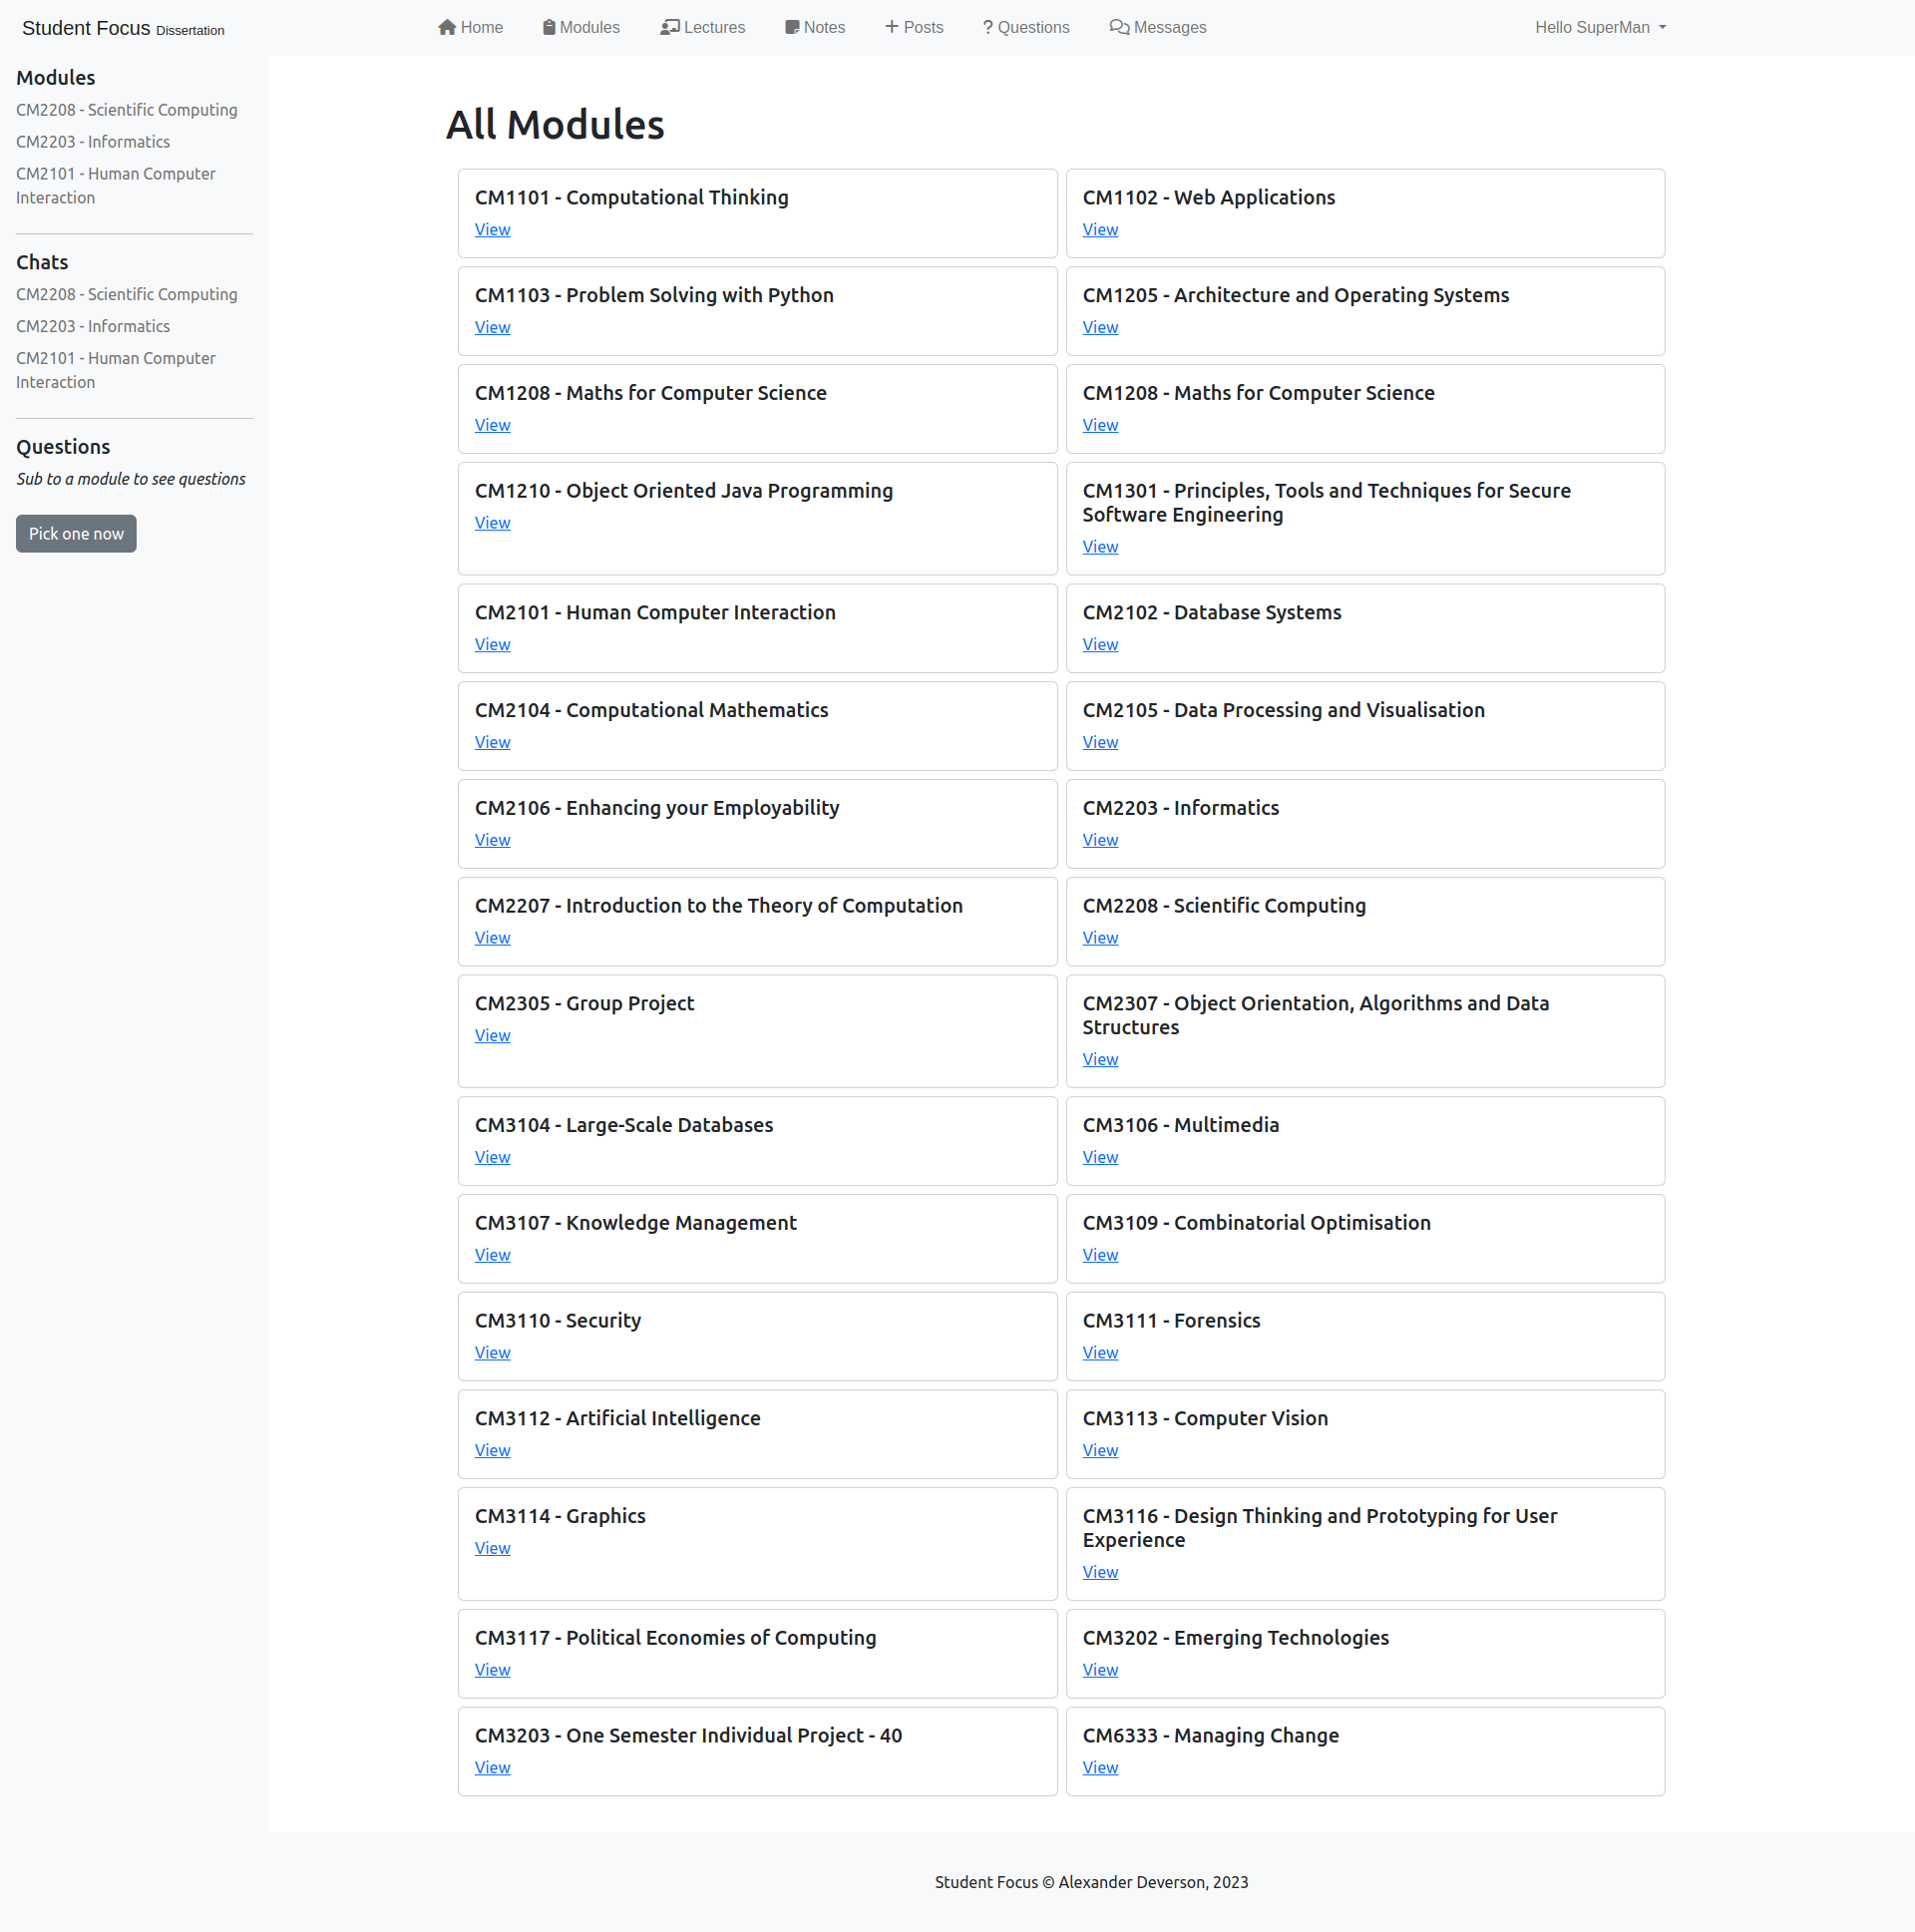
\includegraphics[scale=0.20]{images/application/7 - all_modules.png}

A page displaying all modules

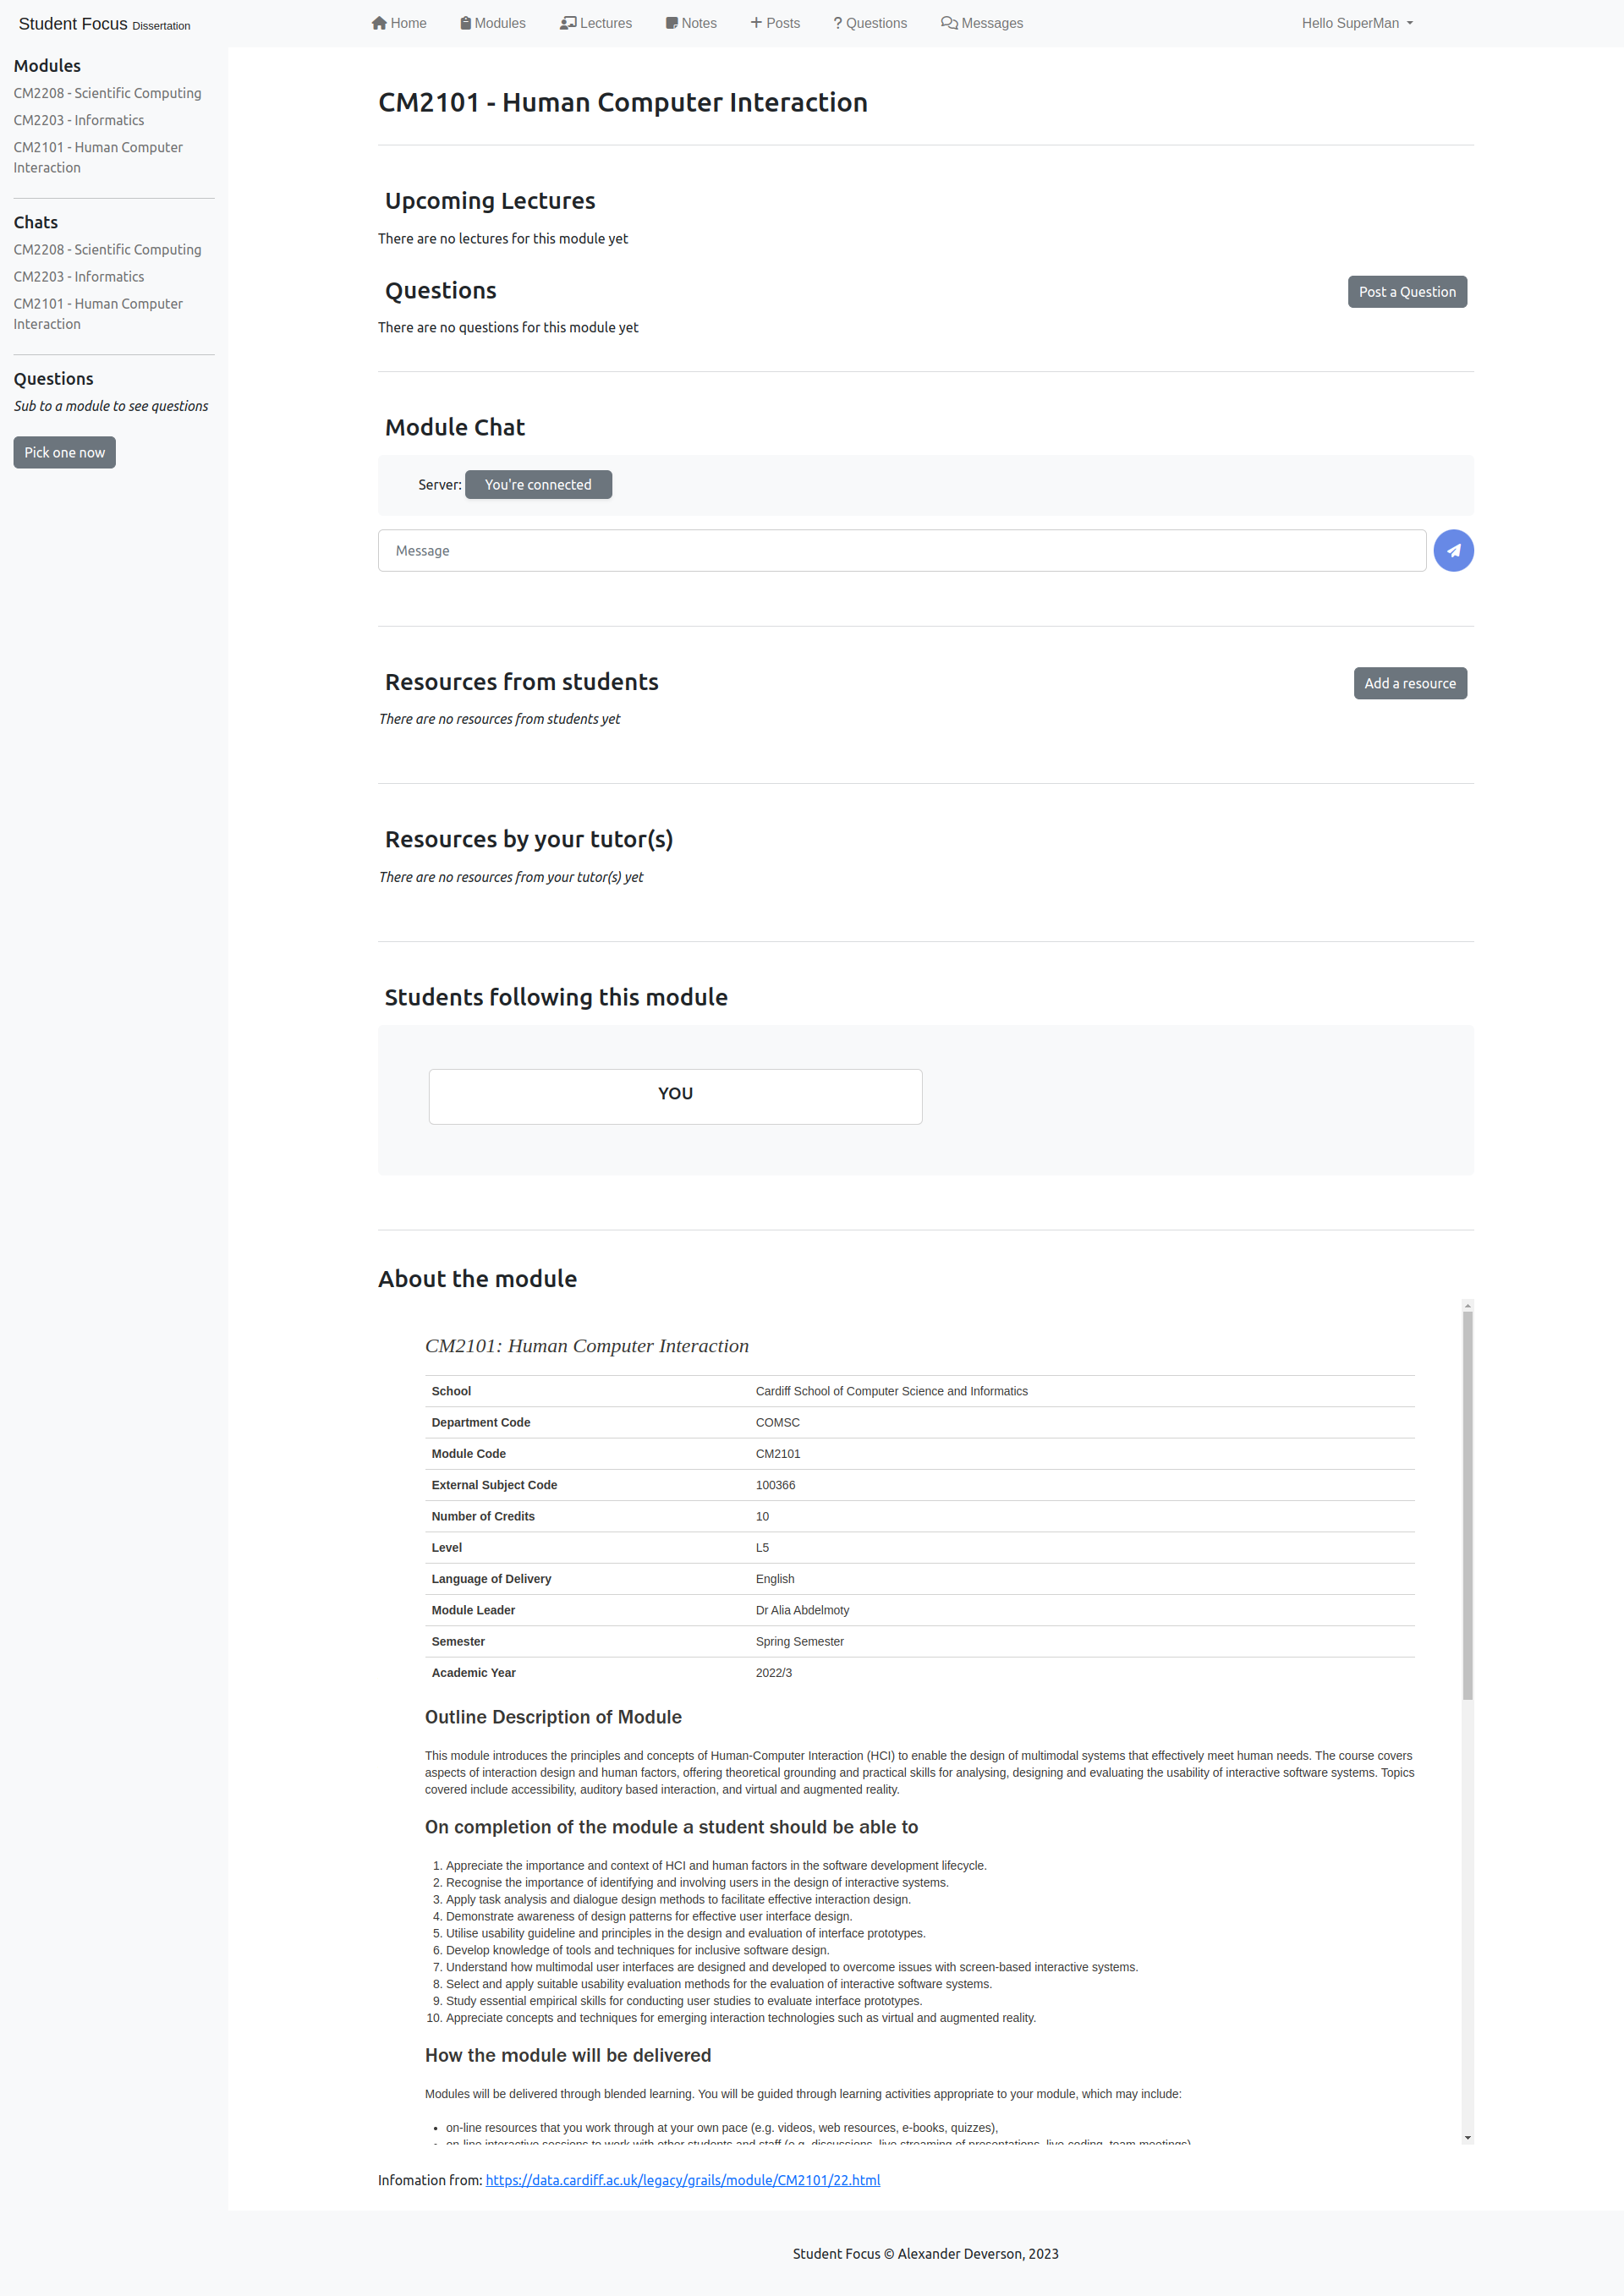
\includegraphics[scale=0.20]{images/application/8 - modules_single_empty.png}

Brand new page for a single module

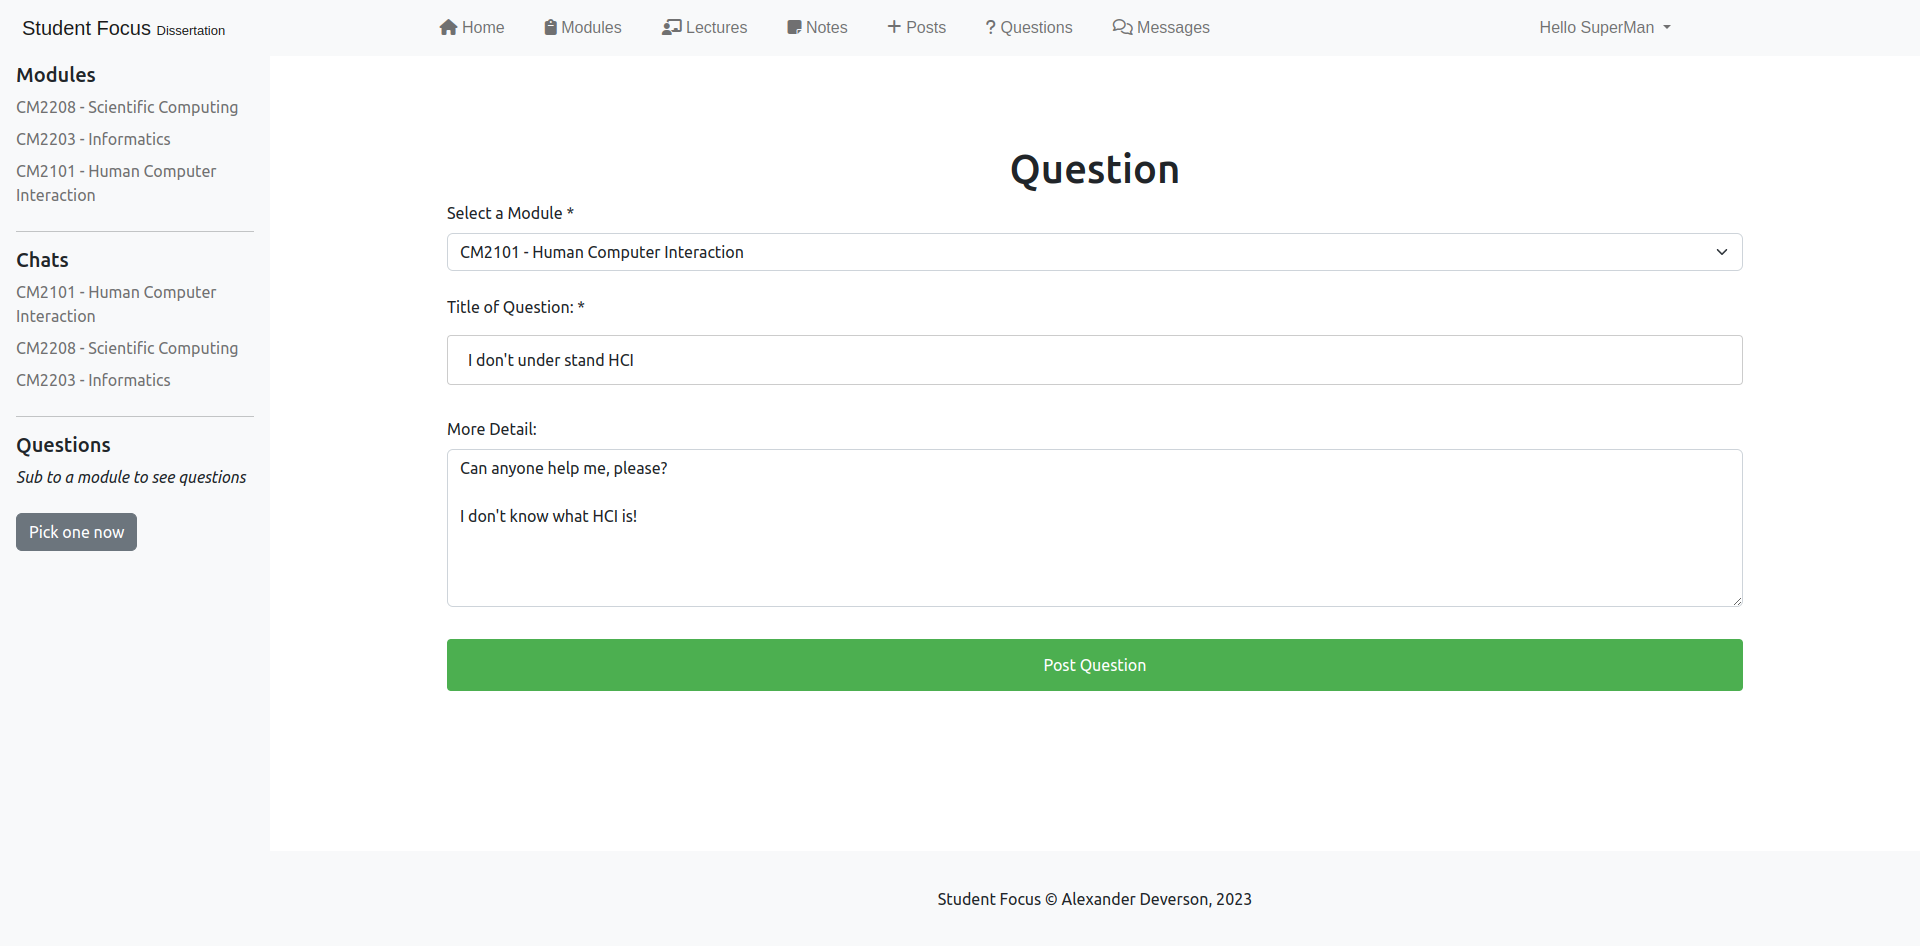
\includegraphics[scale=0.20]{images/application/9 - new question.png}

New question form page

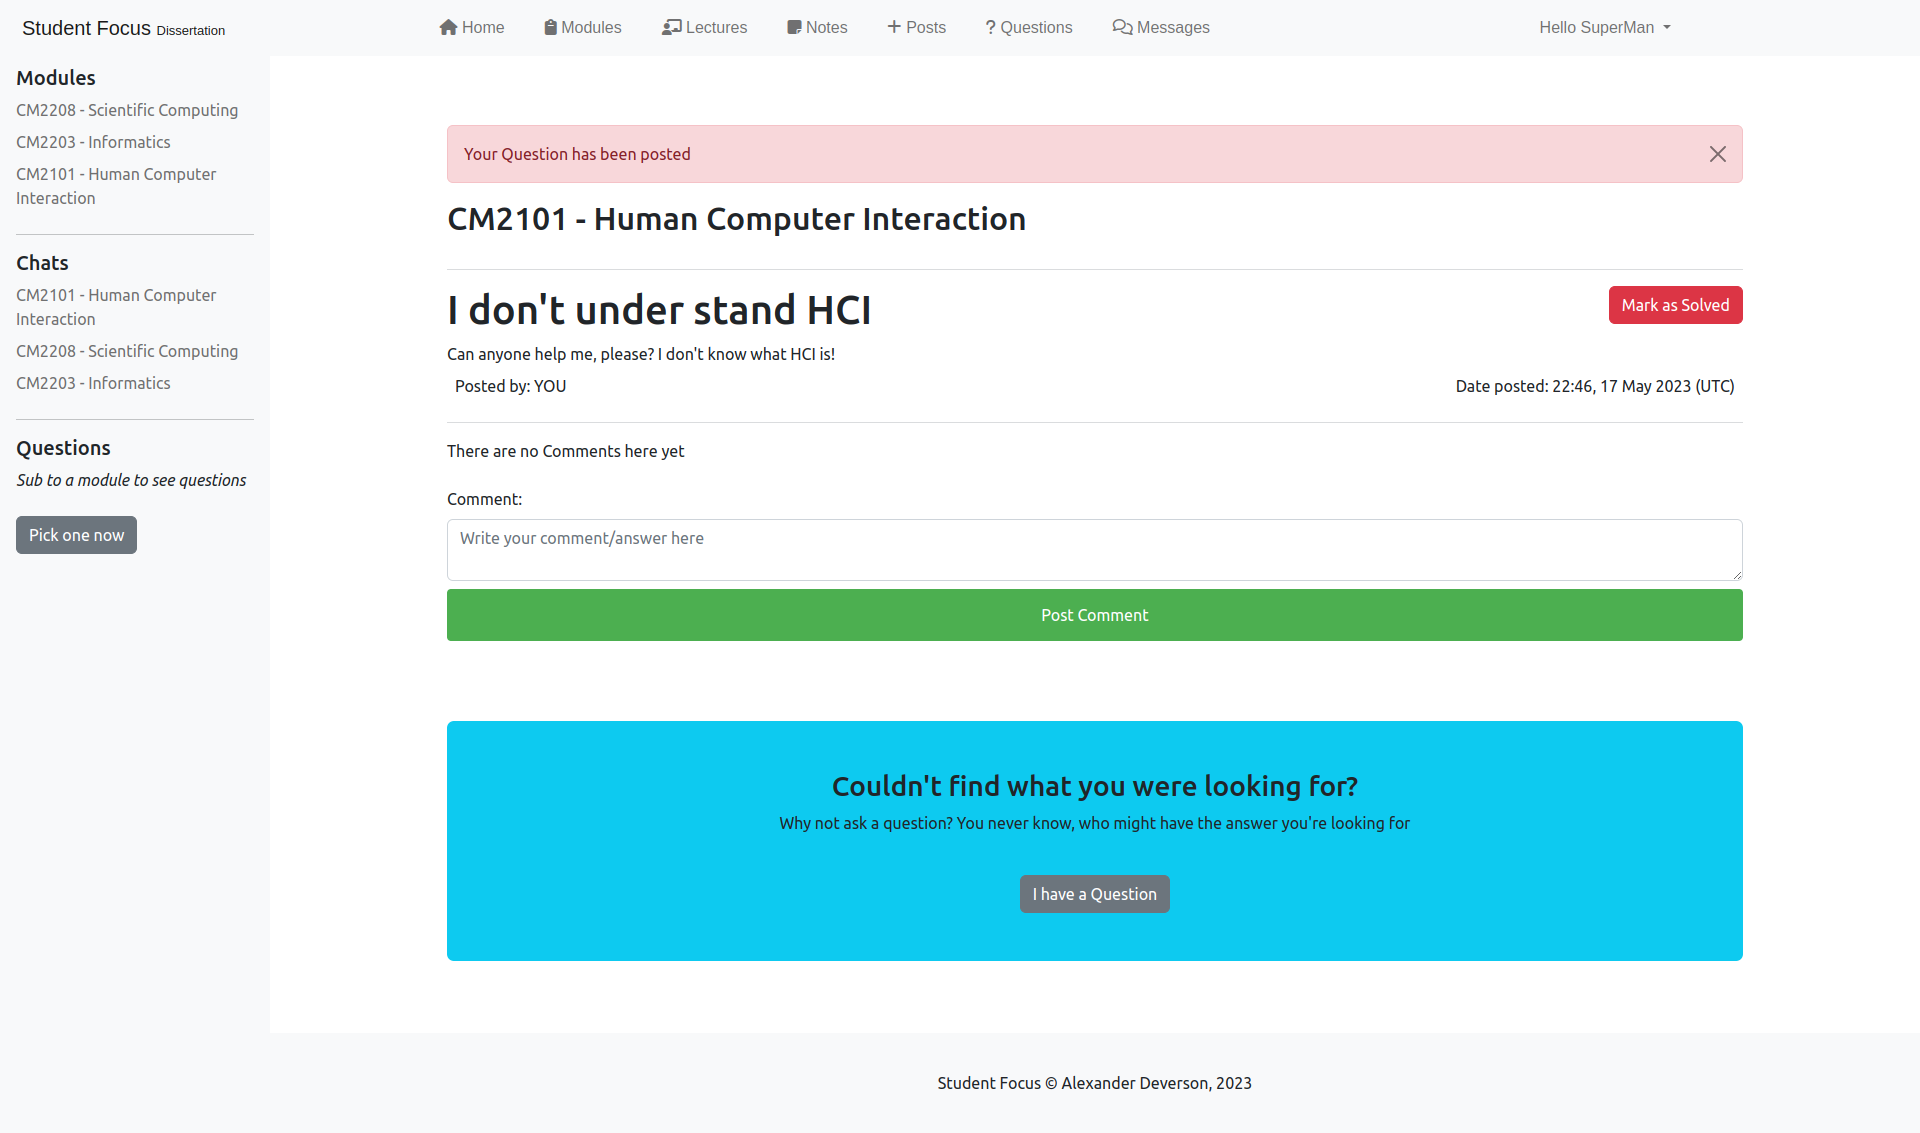
\includegraphics[scale=0.20]{images/application/10 - question posted.png}

Page showing a single question after it has been posted

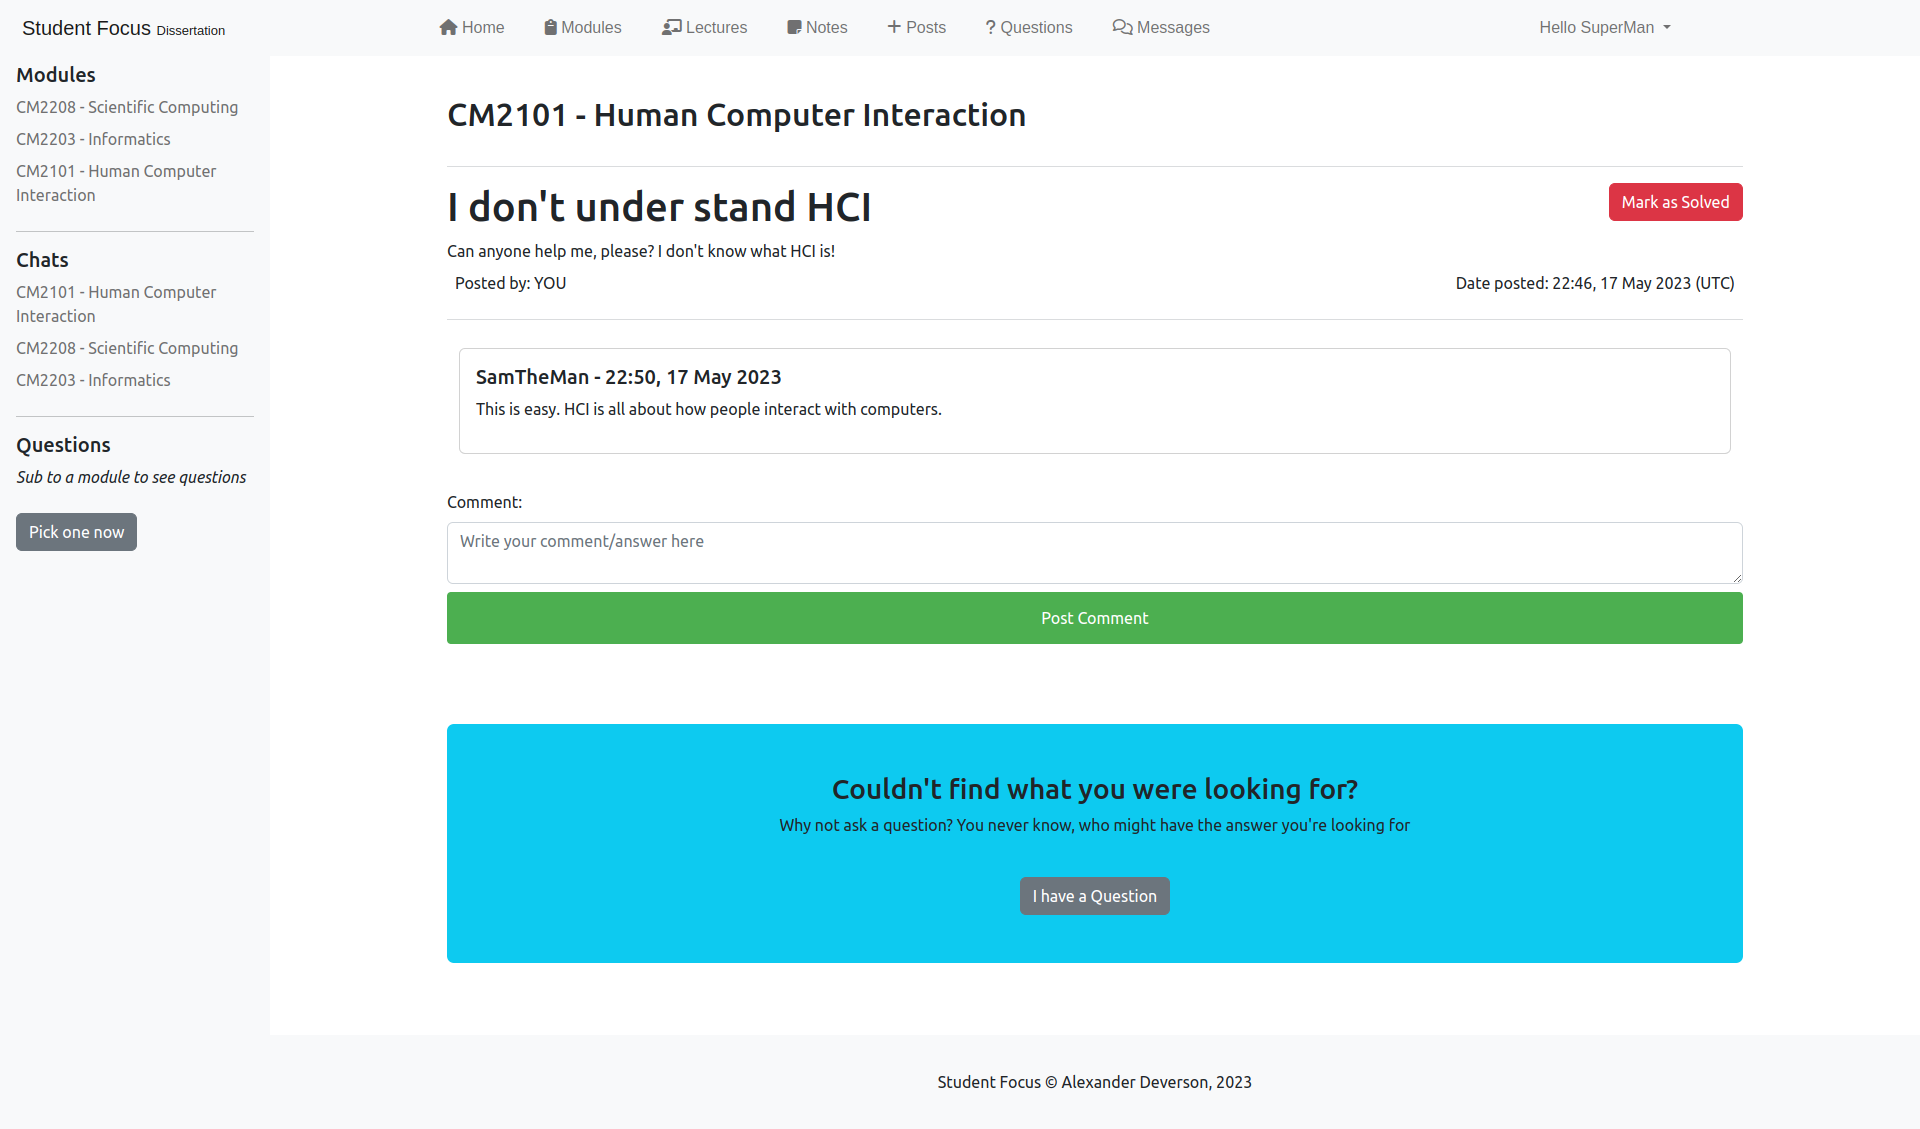
\includegraphics[scale=0.20]{images/application/11 - question_comment.png}

Single question page with a comment

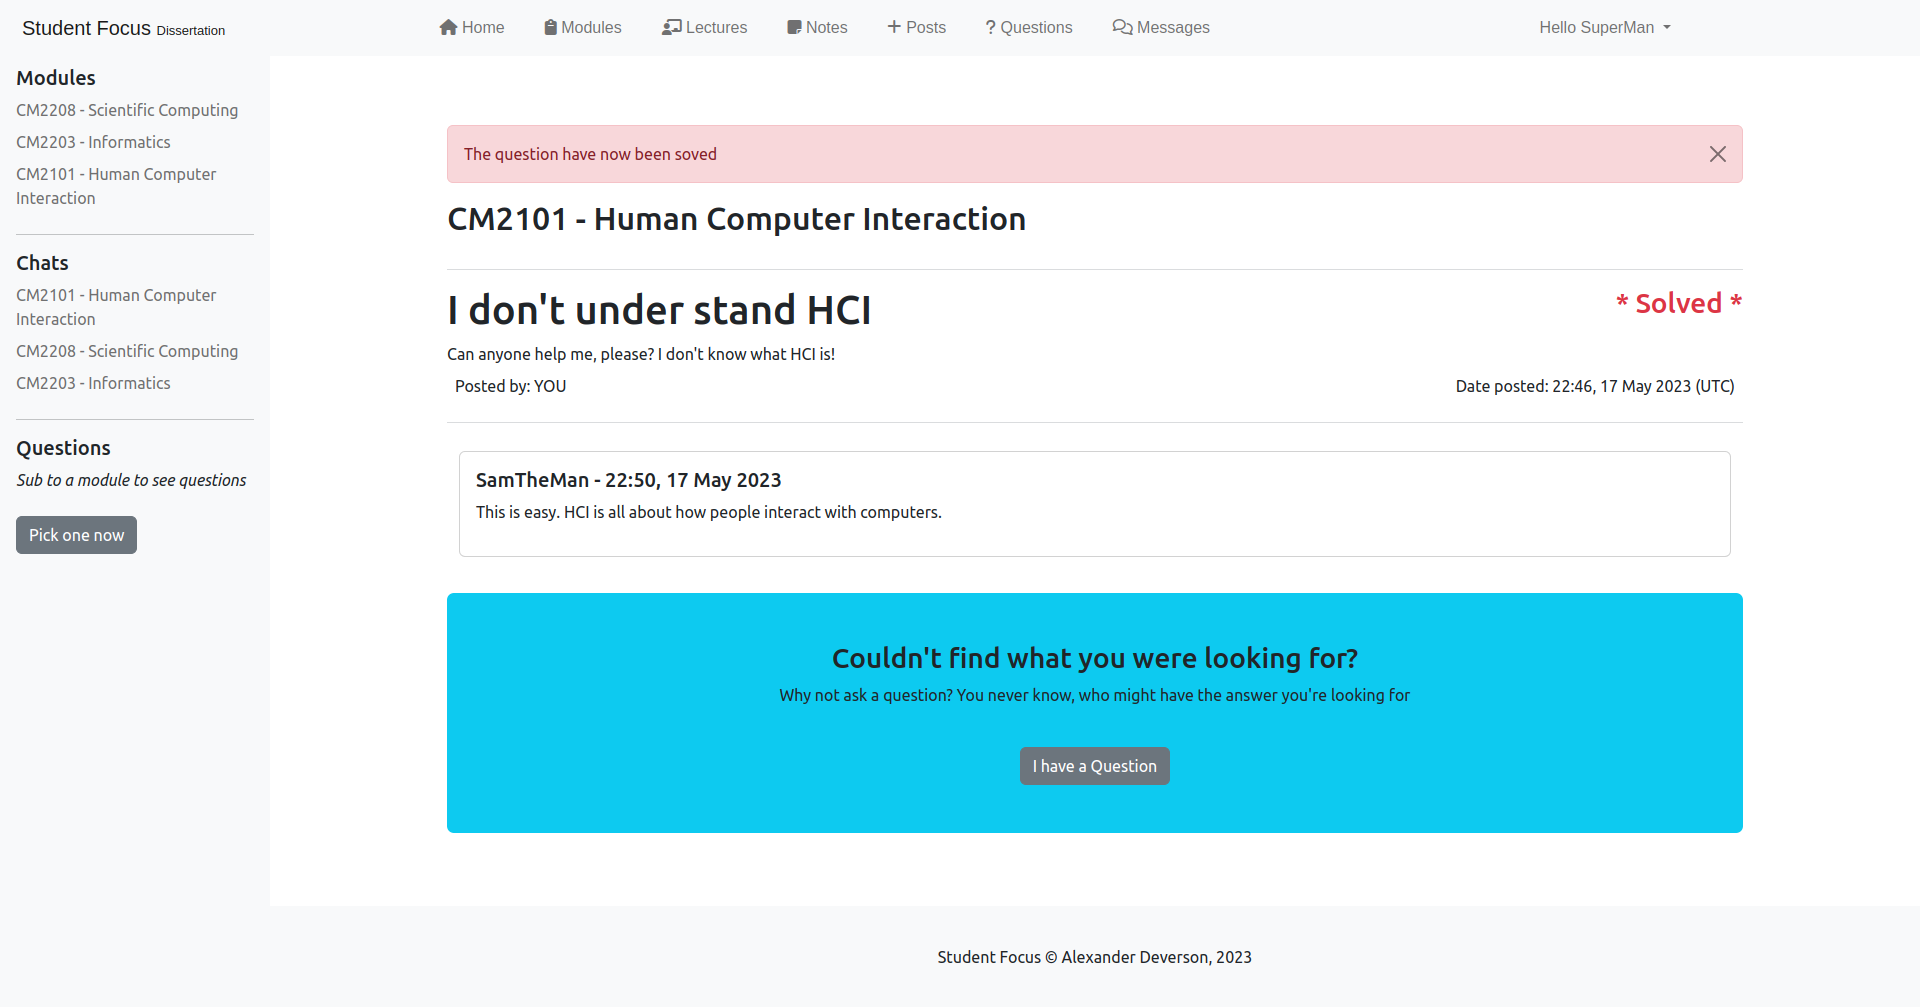
\includegraphics[scale=0.20]{images/application/12 - question_solved.png}

Single question page after the question has been solved

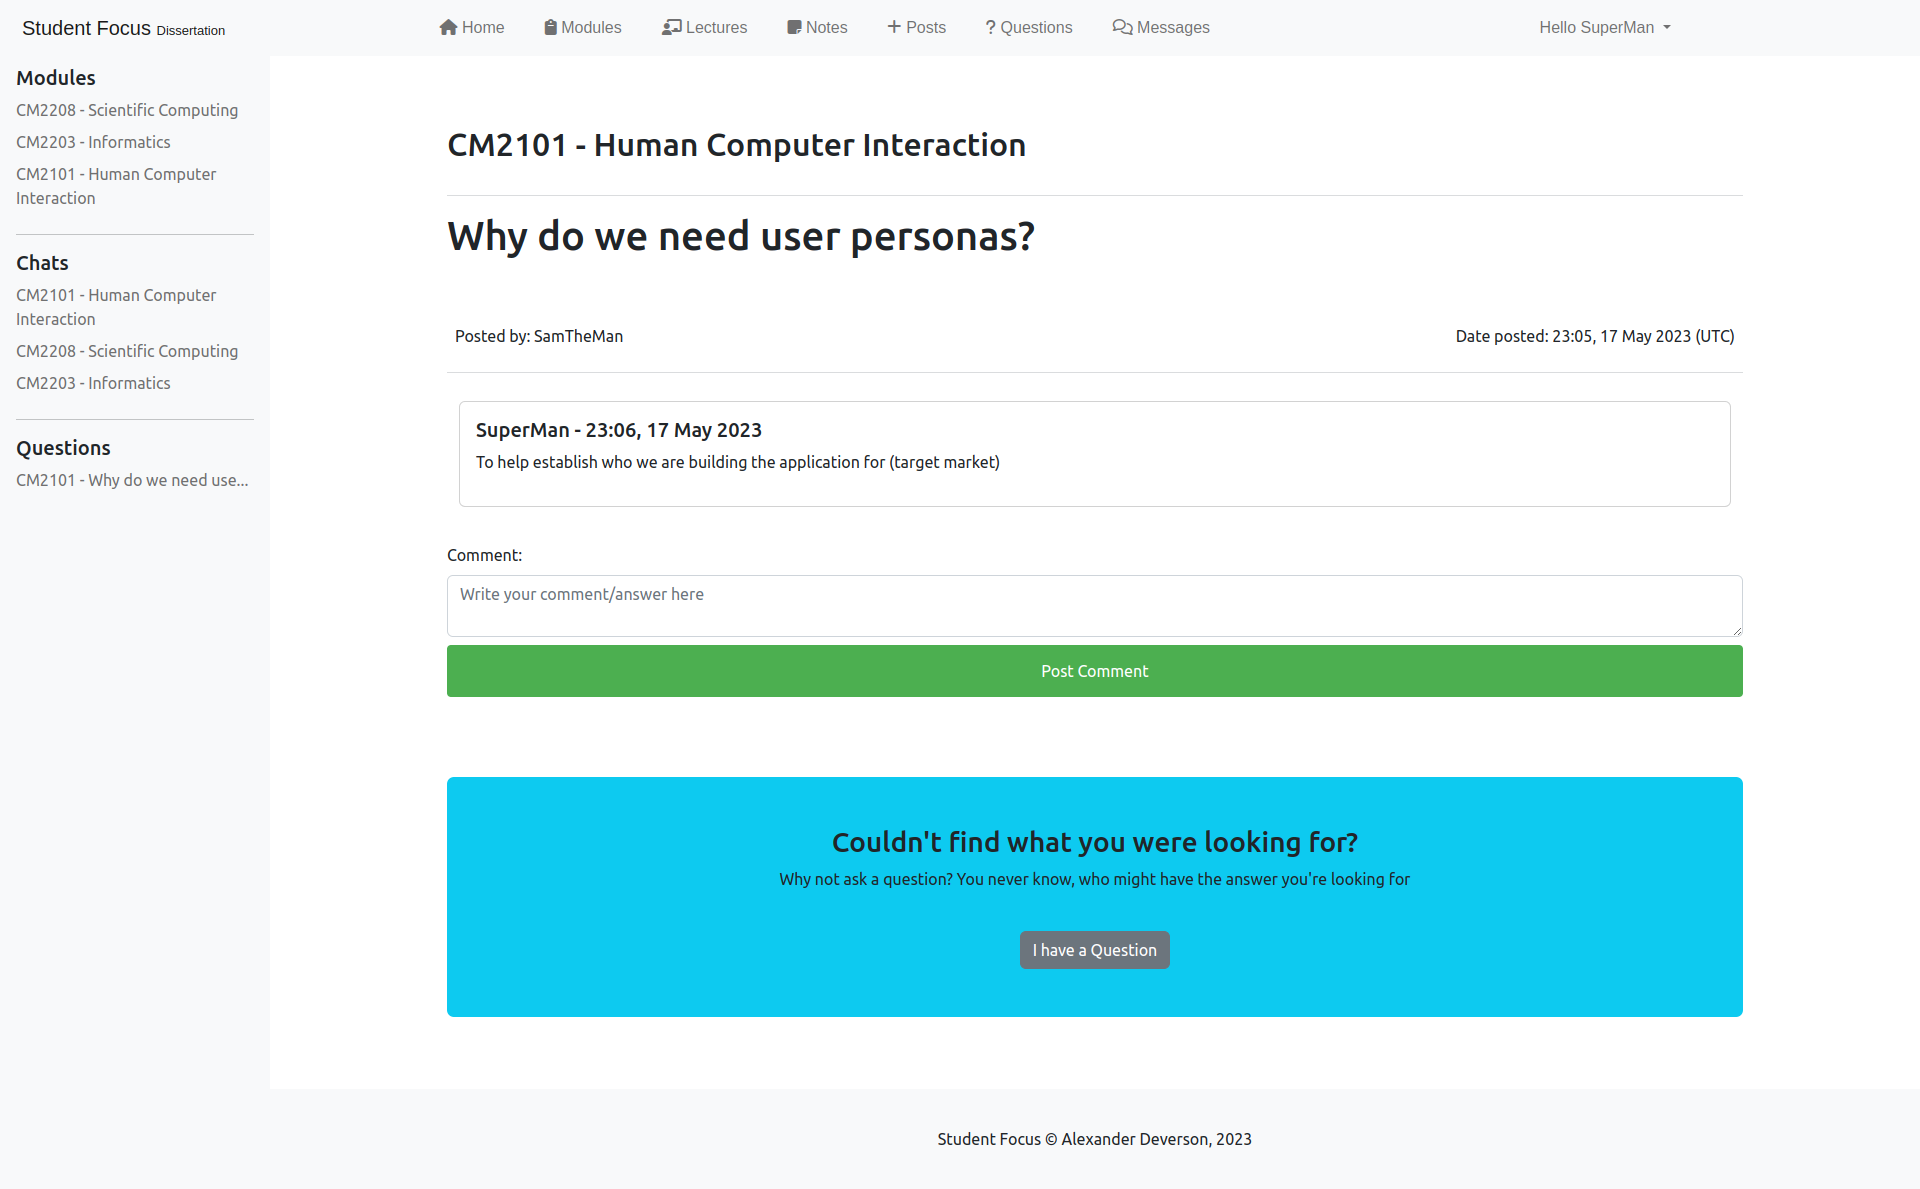
\includegraphics[scale=0.20]{images/application/13 - other users question.png}

Single question page showing a different user's question

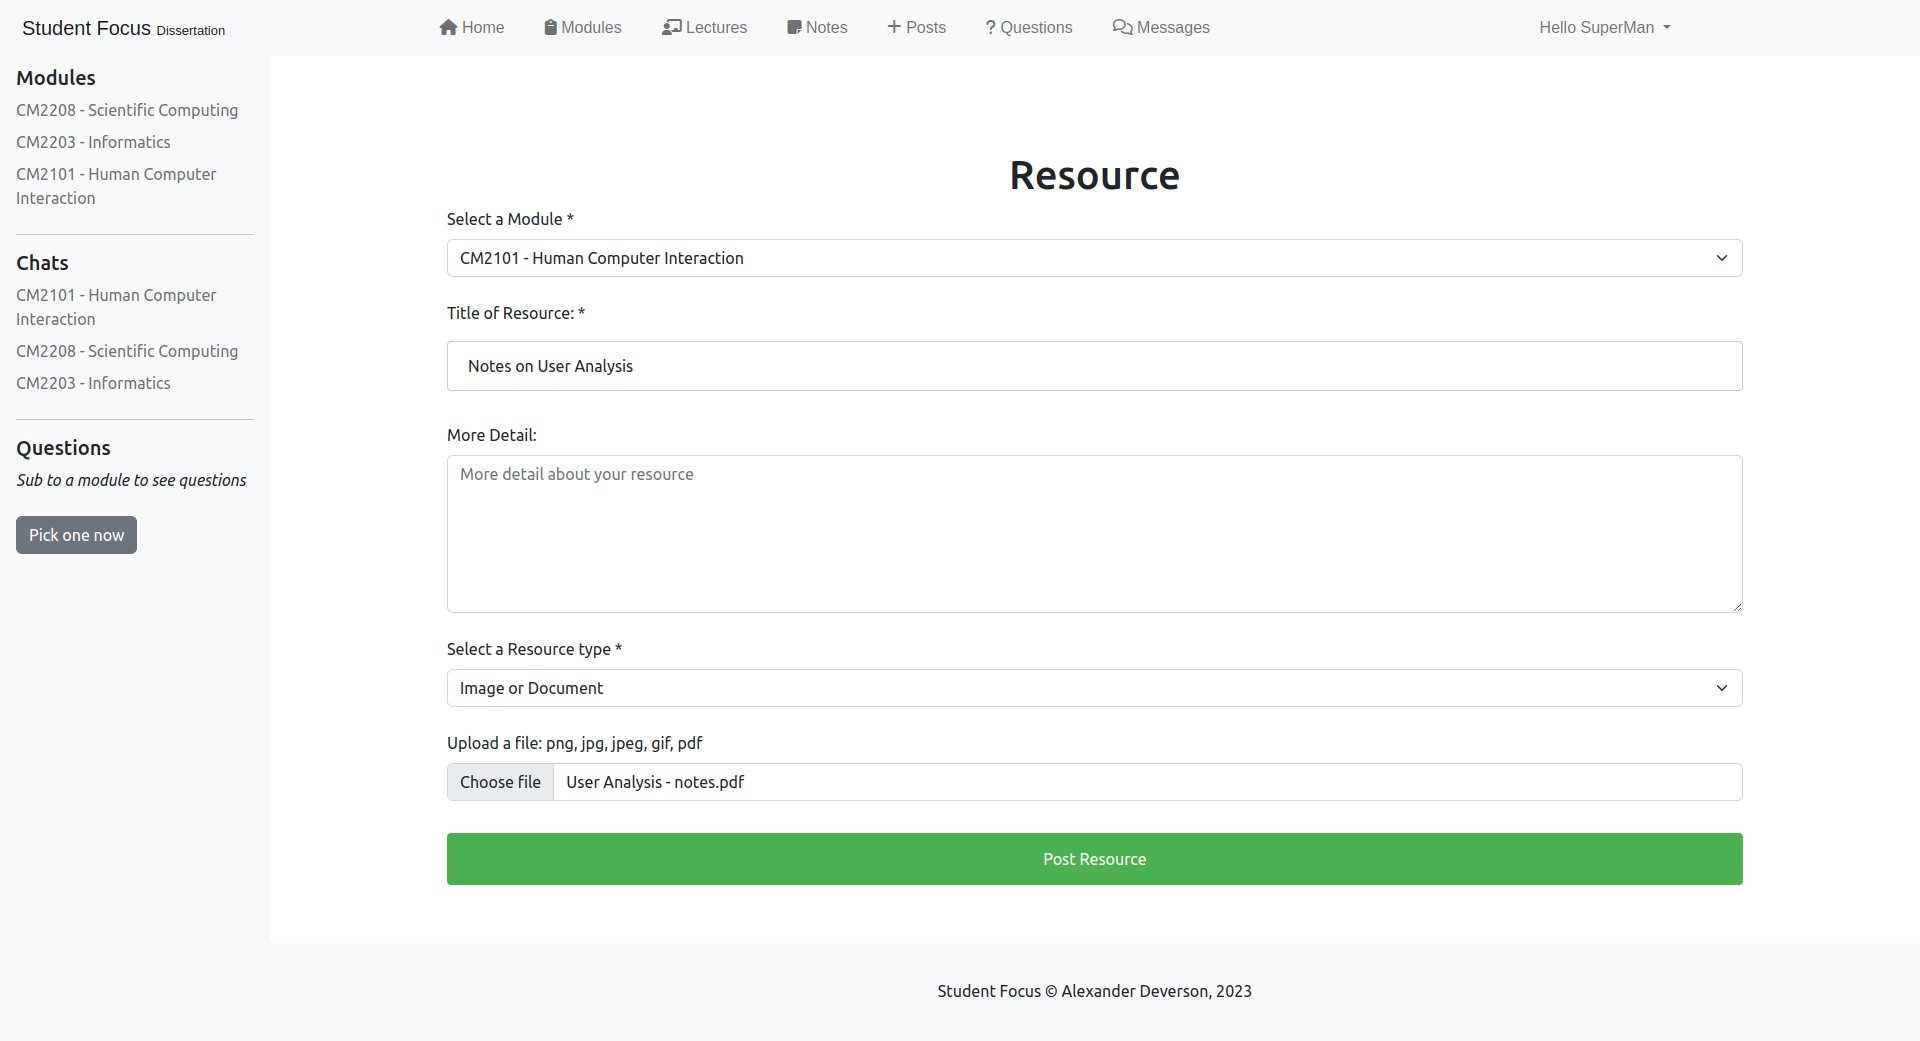
\includegraphics[scale=0.20]{images/application/14 - student resource.png}

New module resource form page

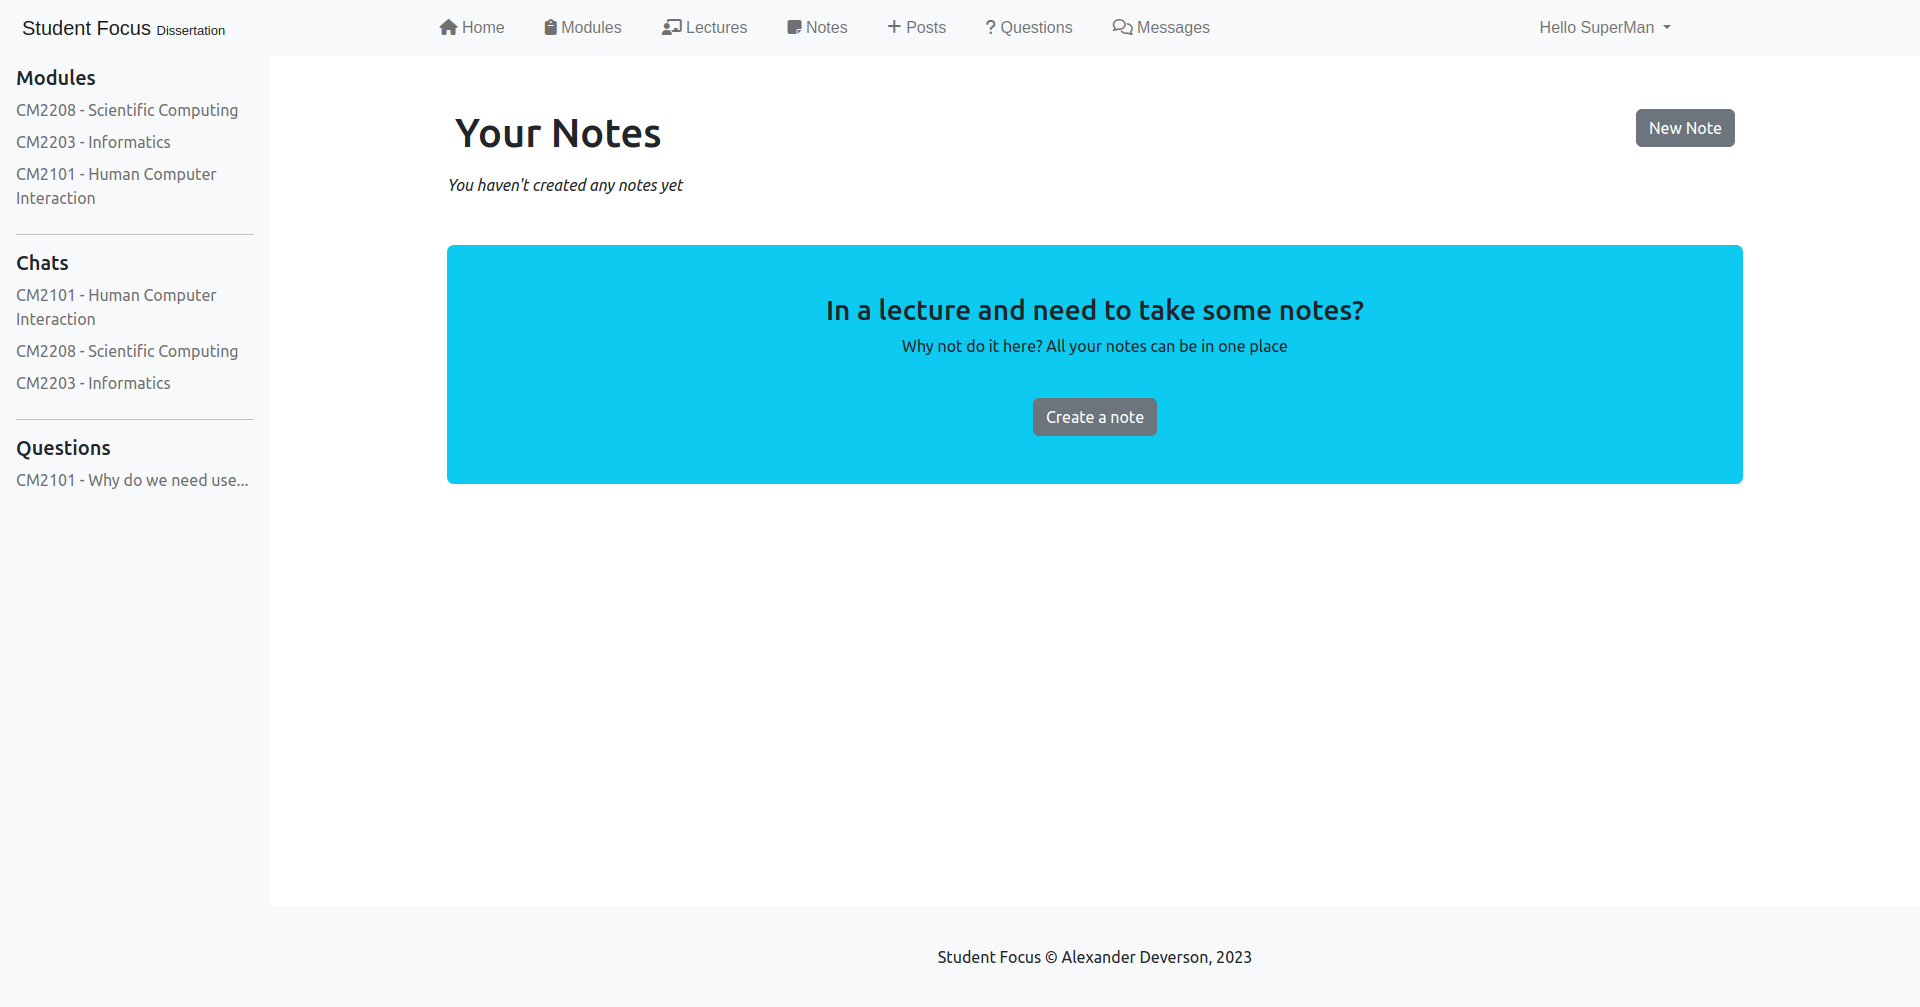
\includegraphics[scale=0.20]{images/application/15 - notes_blank.png}

Blank note list page

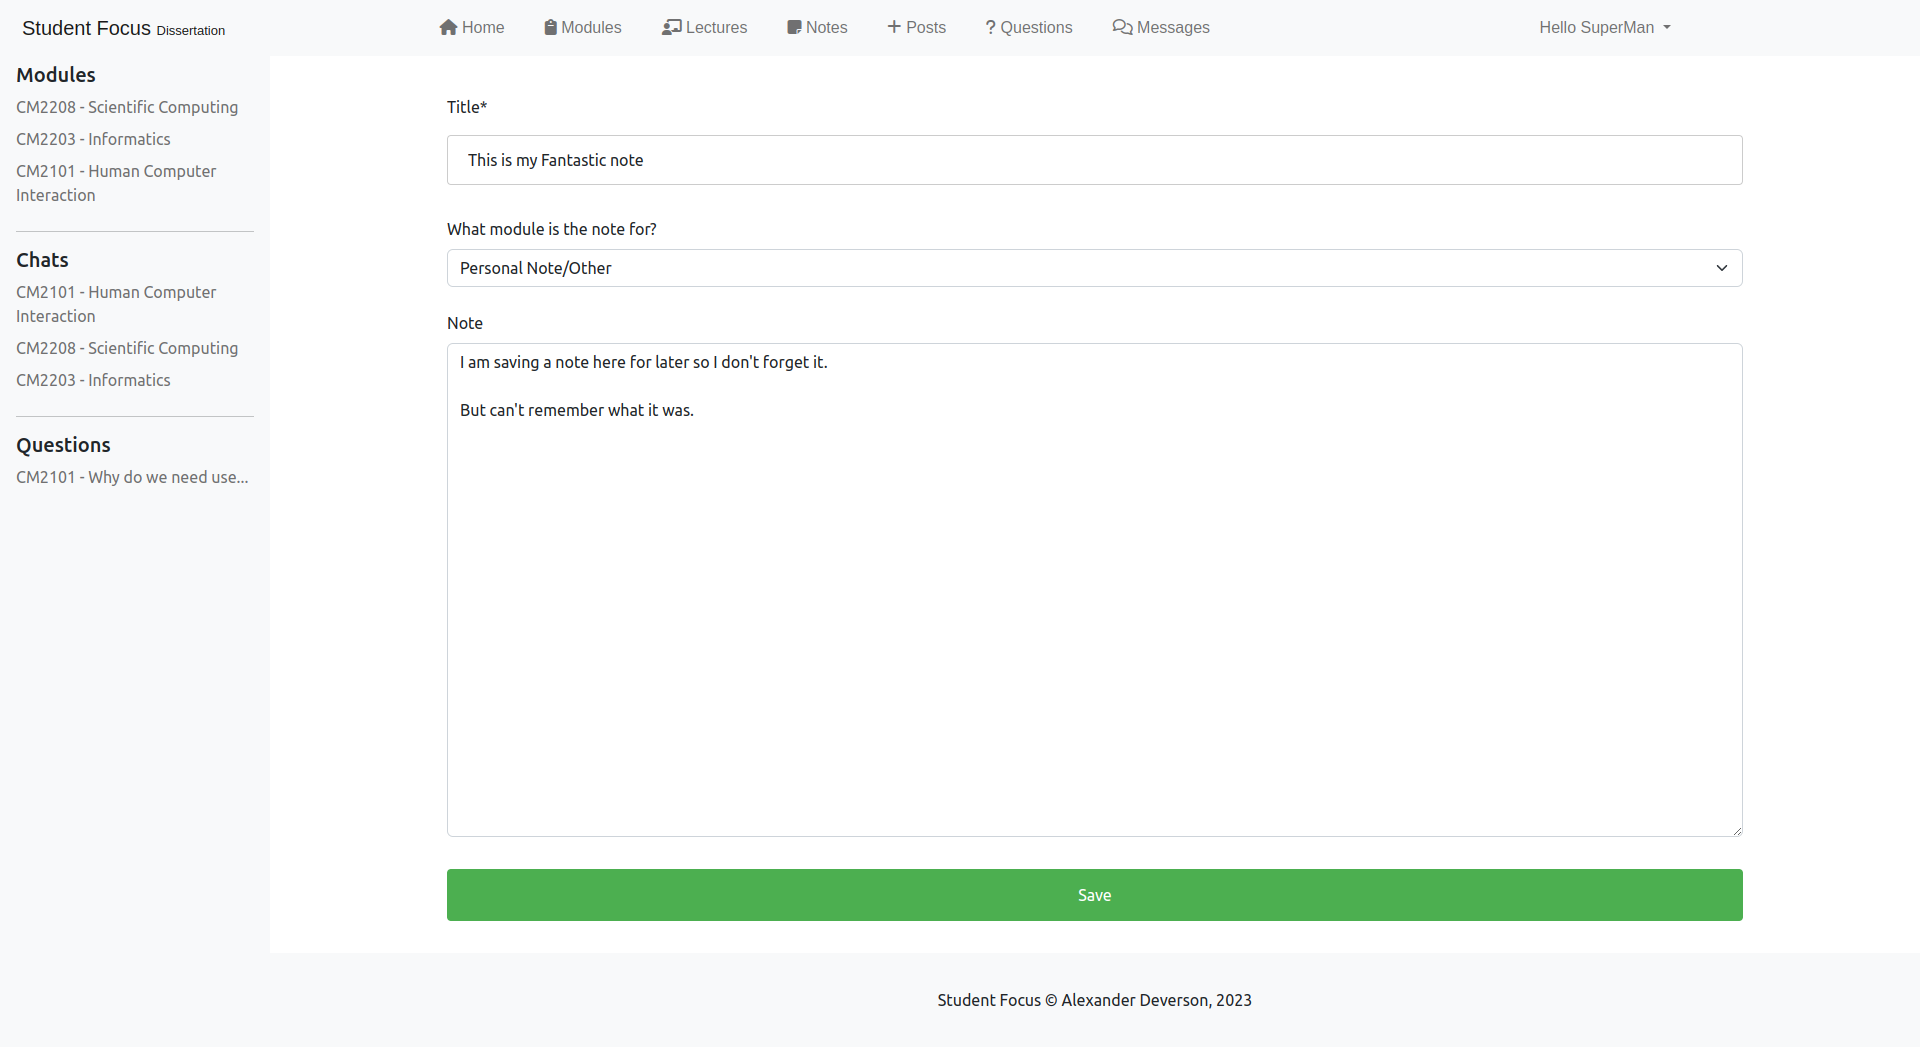
\includegraphics[scale=0.20]{images/application/16 - new_note.png}

A page for adding a new note and updating old notes

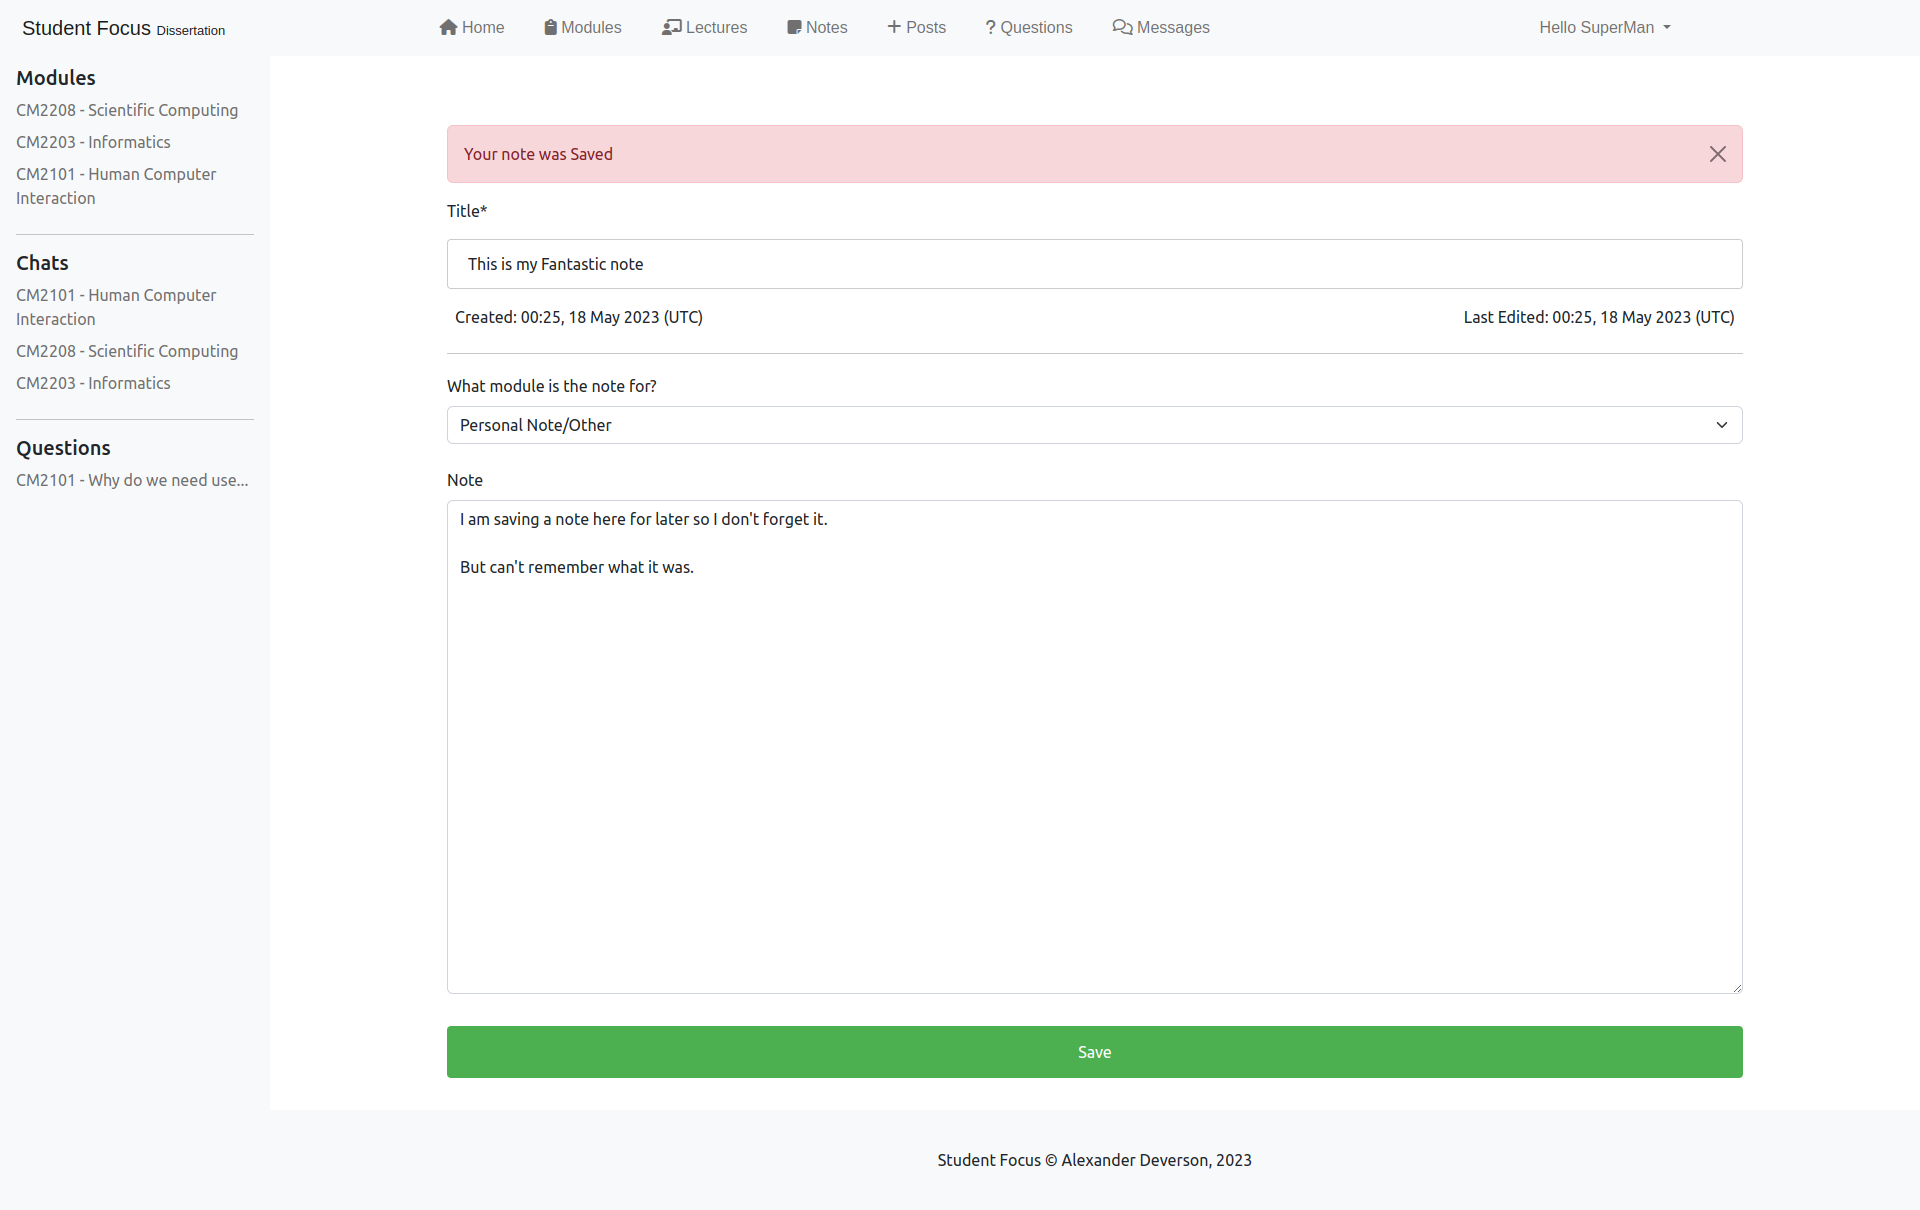
\includegraphics[scale=0.20]{images/application/17 - note_first_save.png}

After a note has been saved for the first time

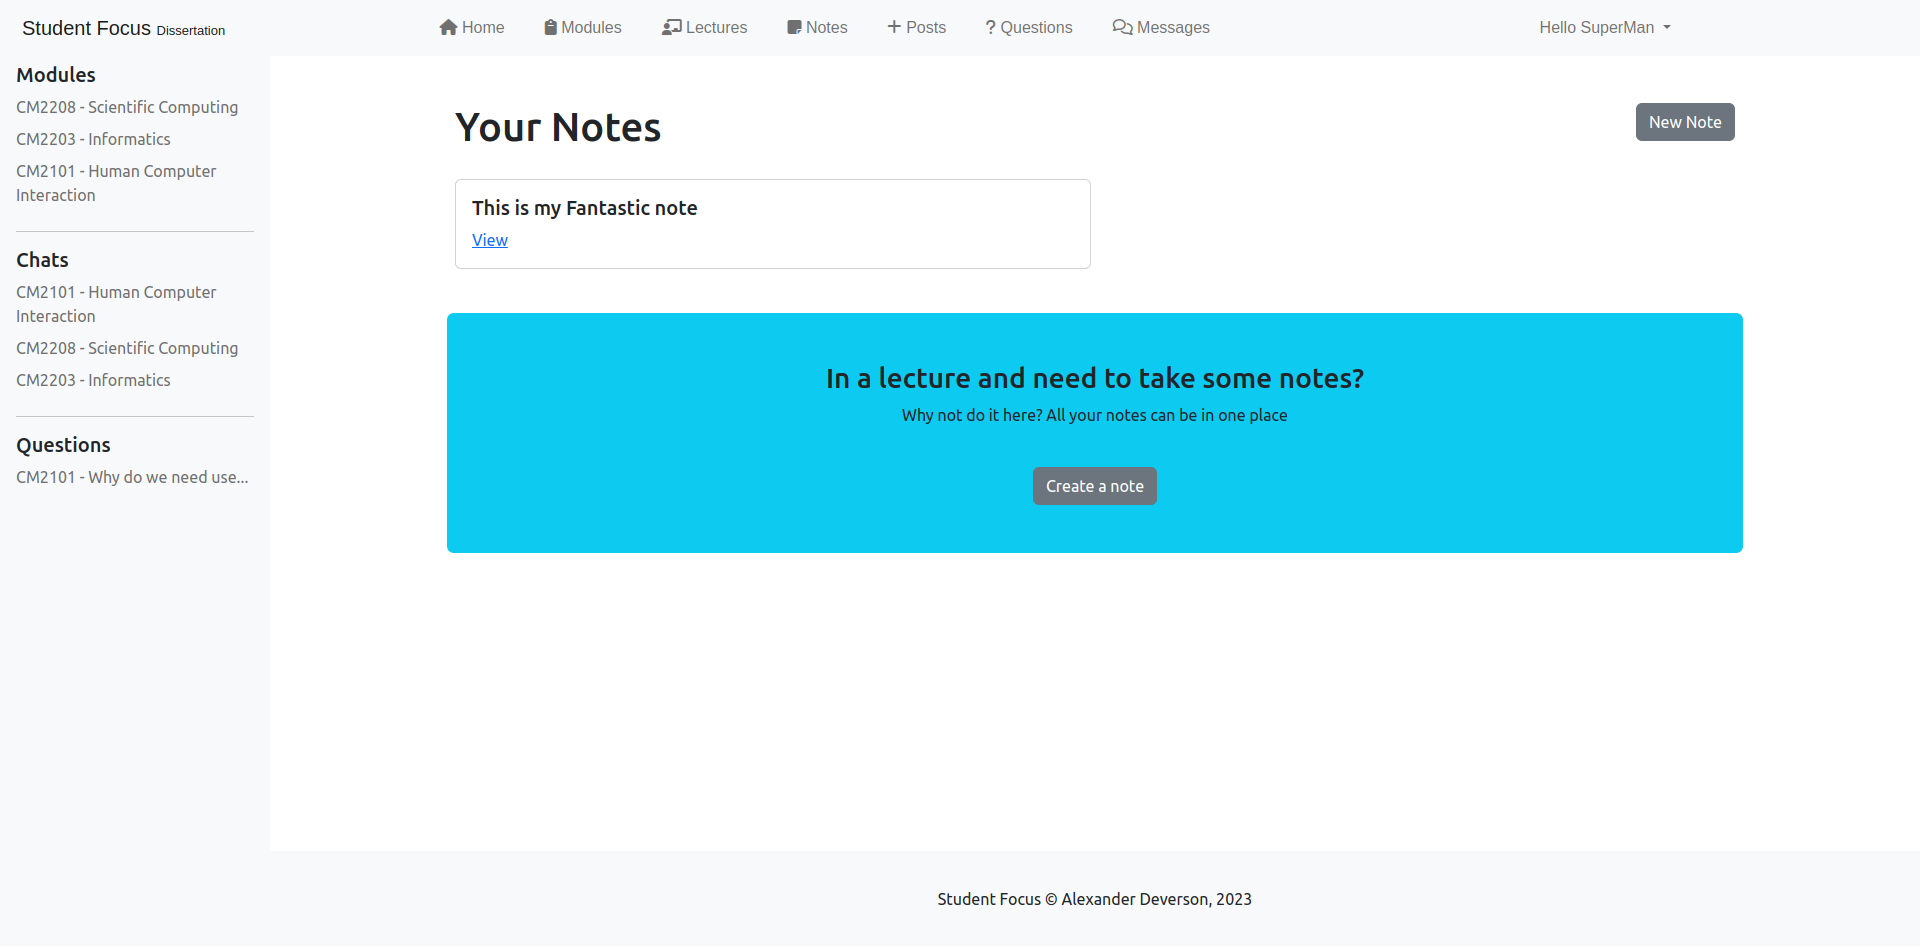
\includegraphics[scale=0.20]{images/application/18 - all_notes_first.png}

List of notes after the first one has been created

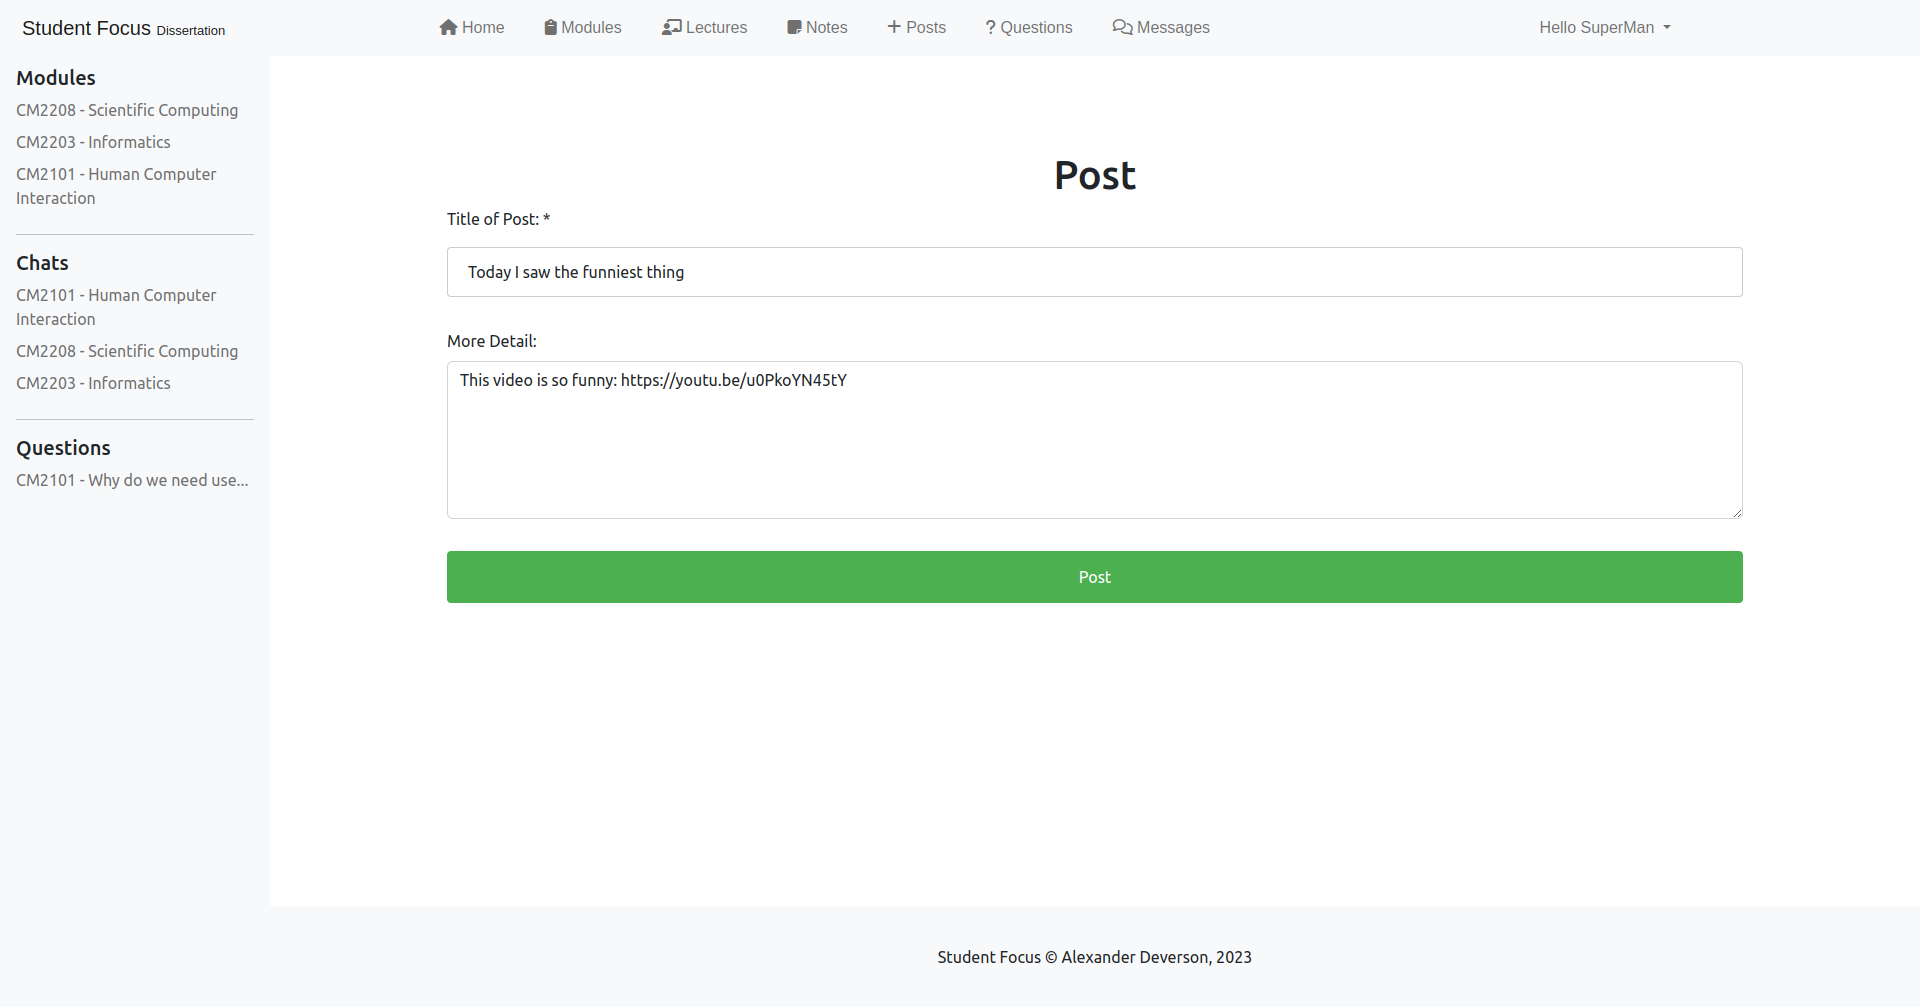
\includegraphics[scale=0.20]{images/application/19 - post_new.png}

New social post form page

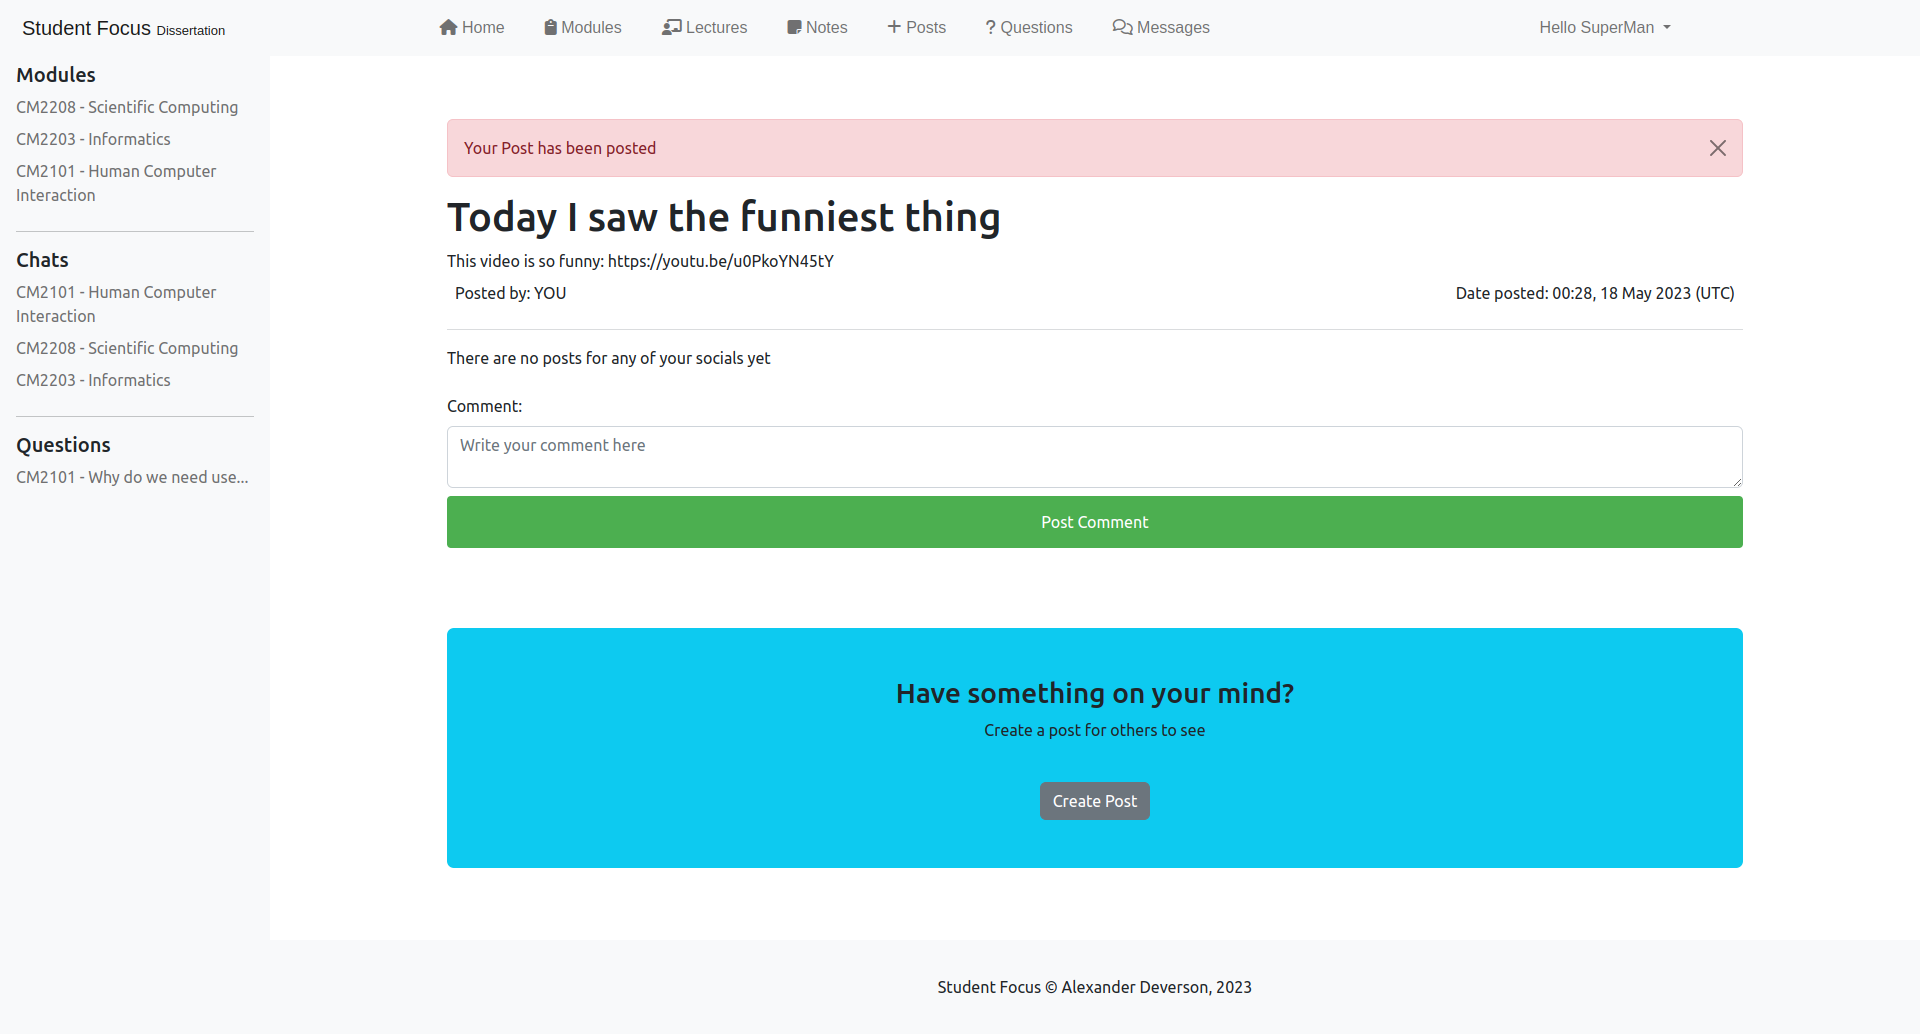
\includegraphics[scale=0.20]{images/application/20 - post_posted.png}

After a social post has been posted

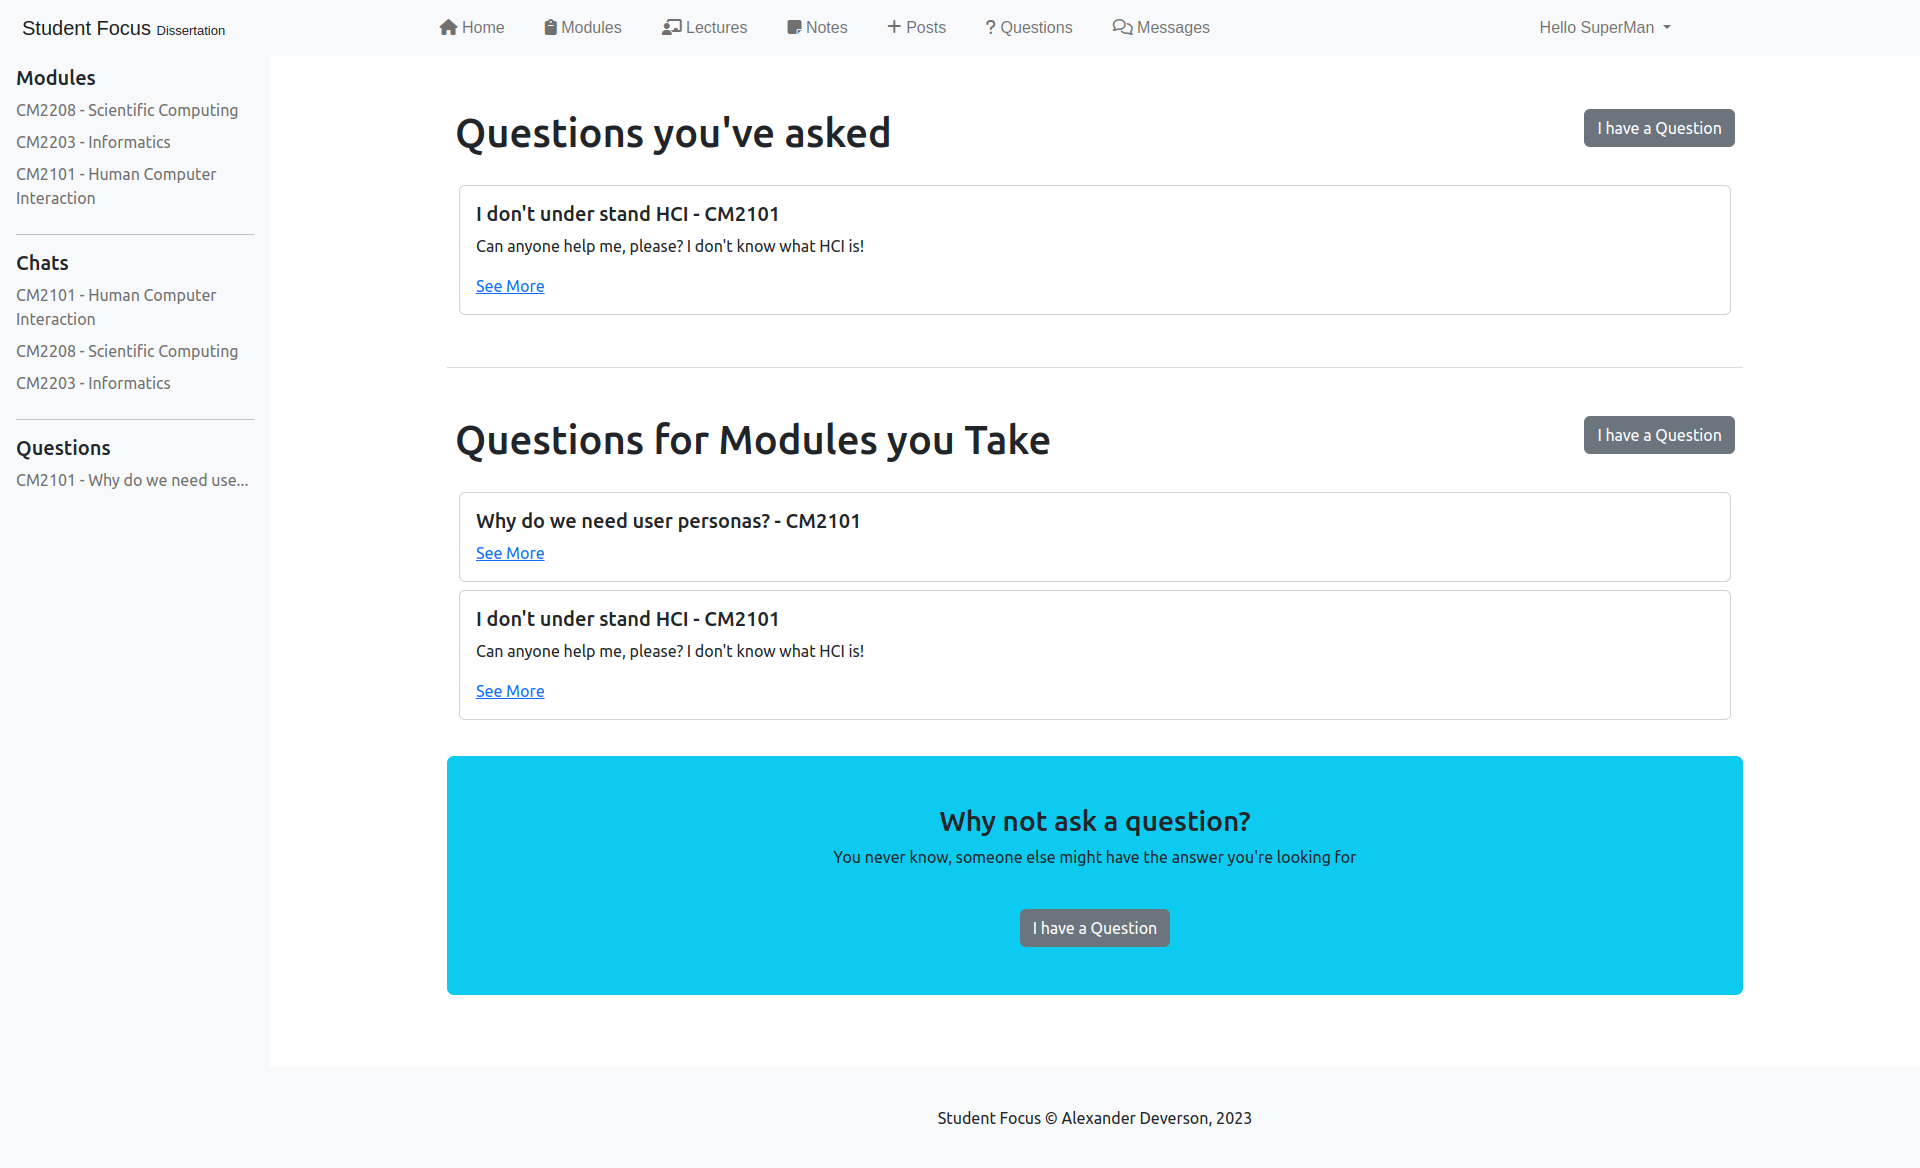
\includegraphics[scale=0.20]{images/application/21 - all_questions.png}

List of questions page

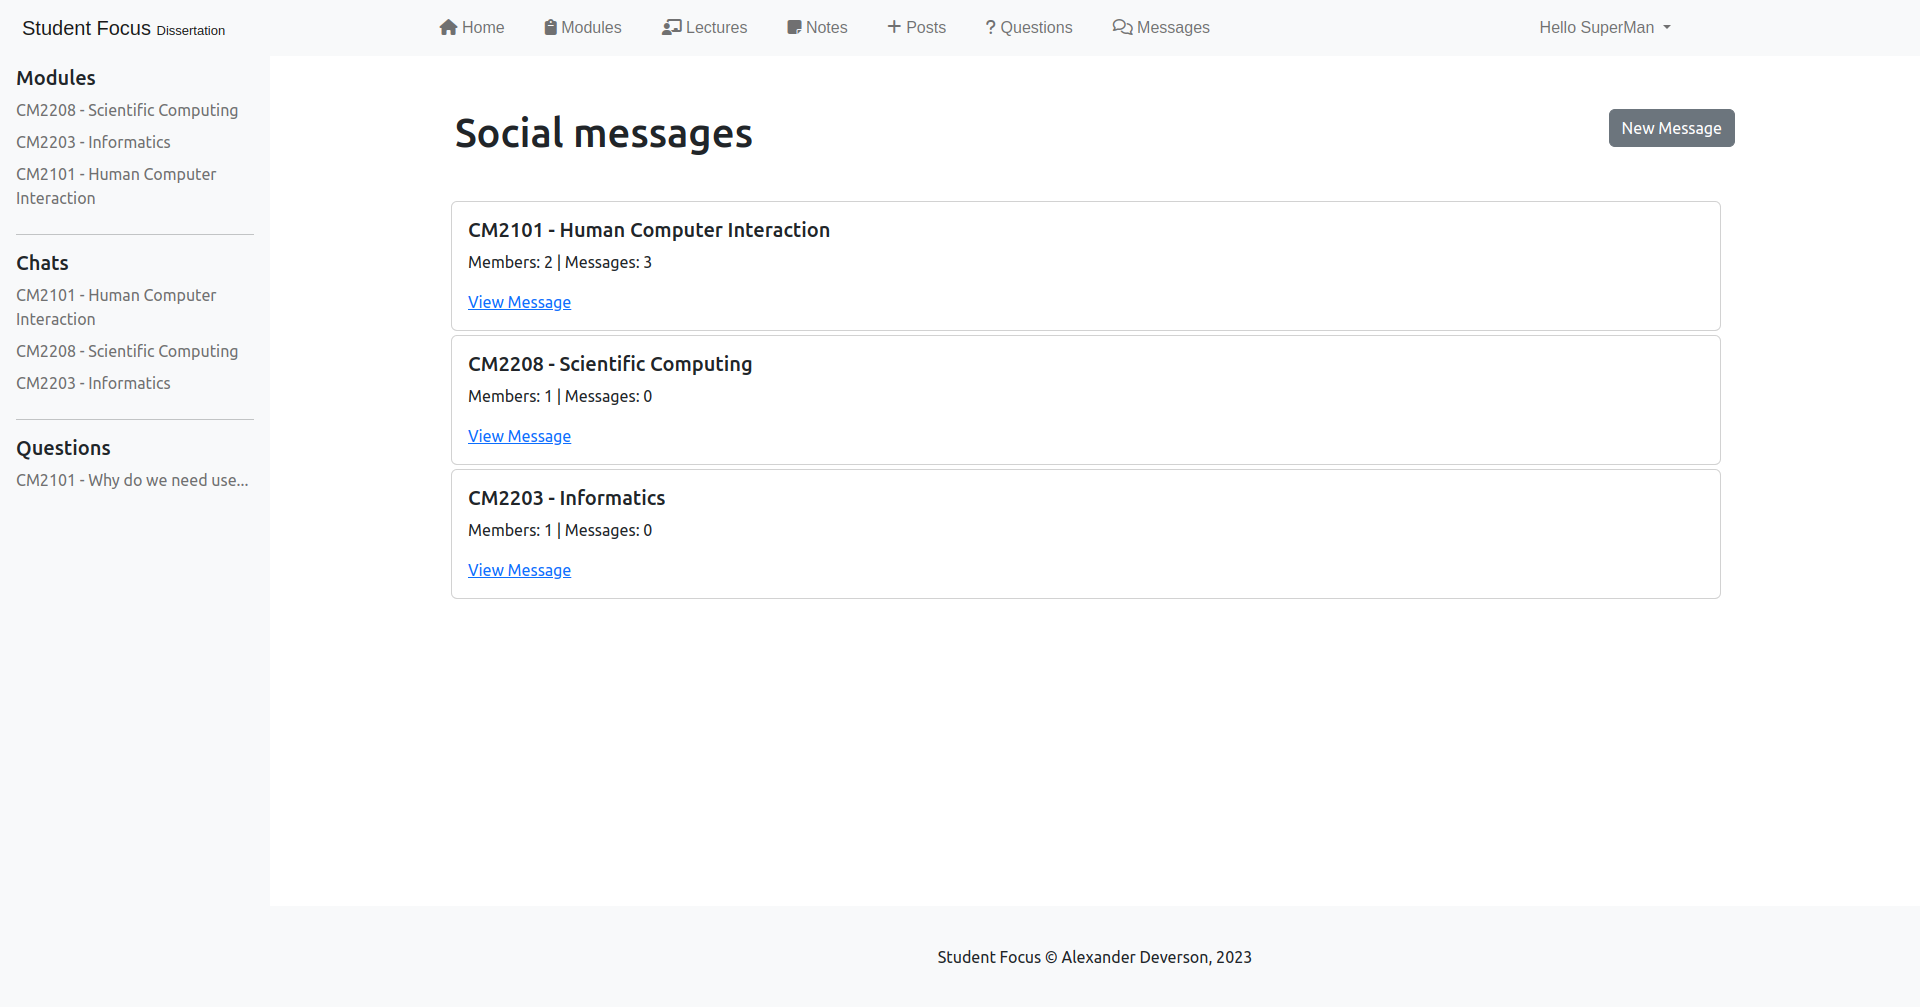
\includegraphics[scale=0.20]{images/application/22 - all_messages.png}

List of all messages page

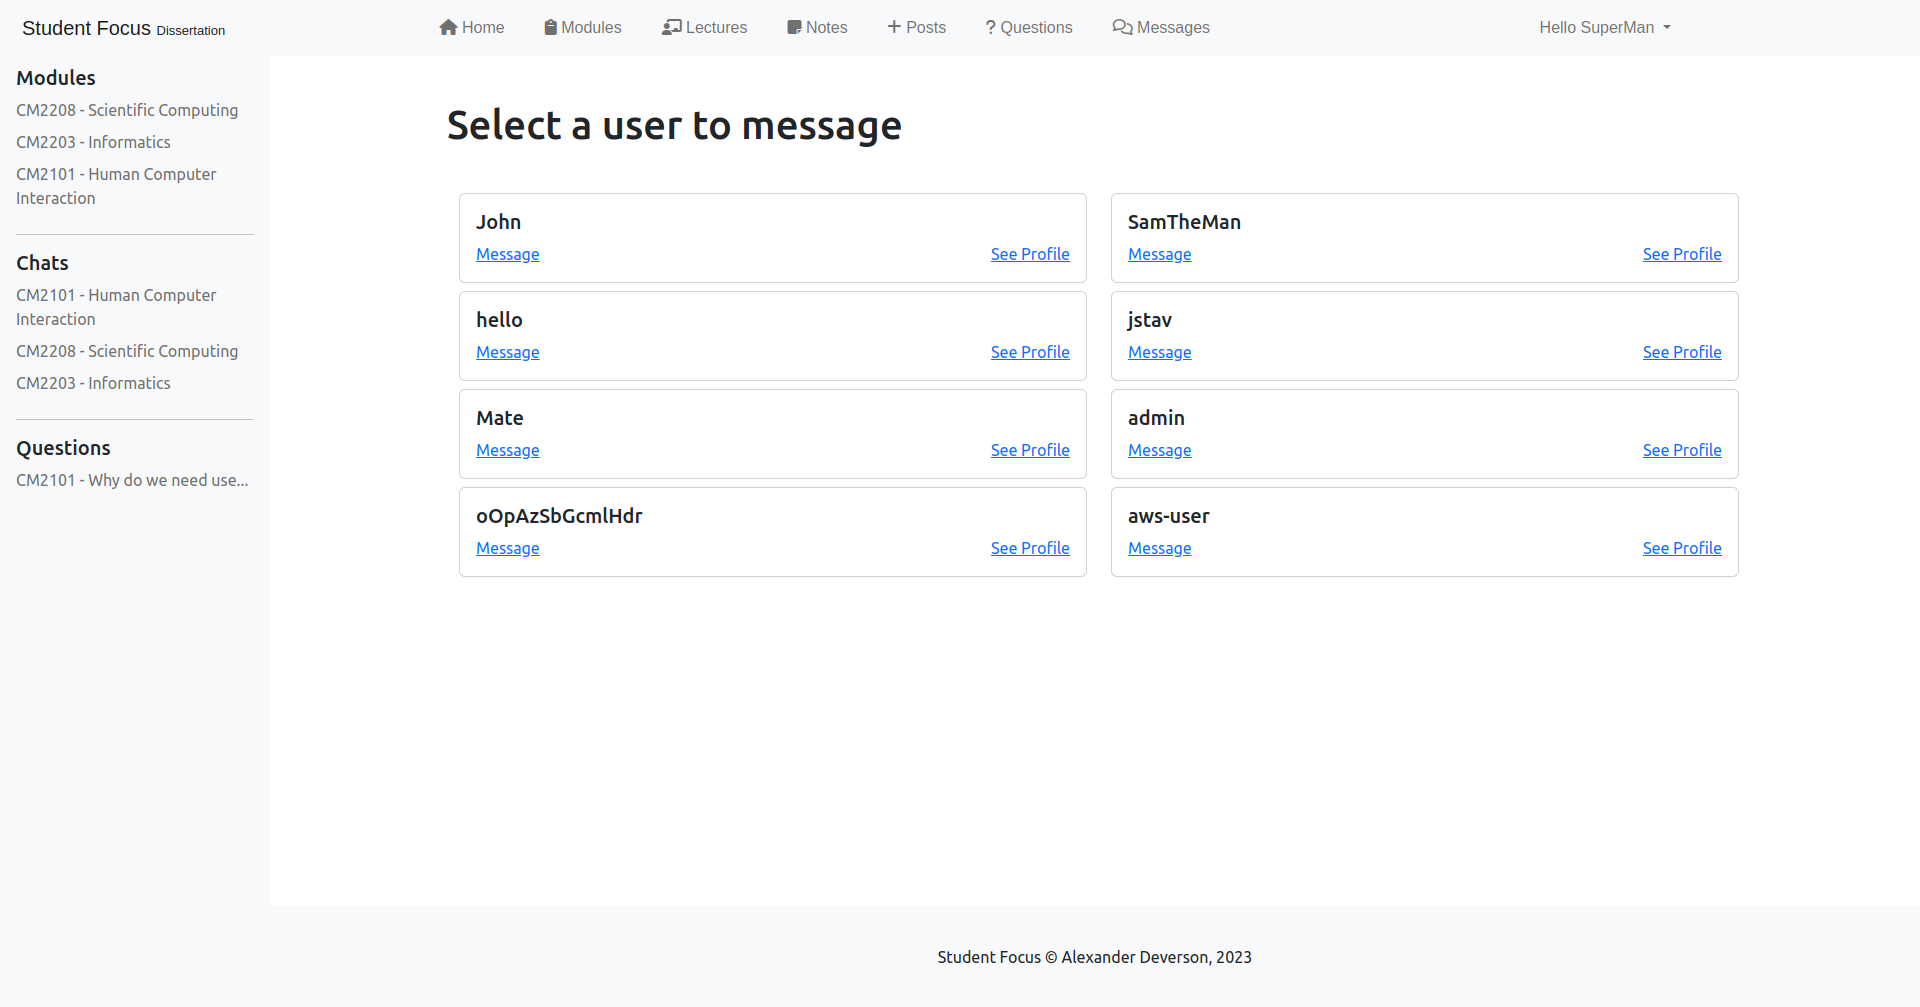
\includegraphics[scale=0.20]{images/application/23 - new_message.png}

A page listing all the users ready to message them

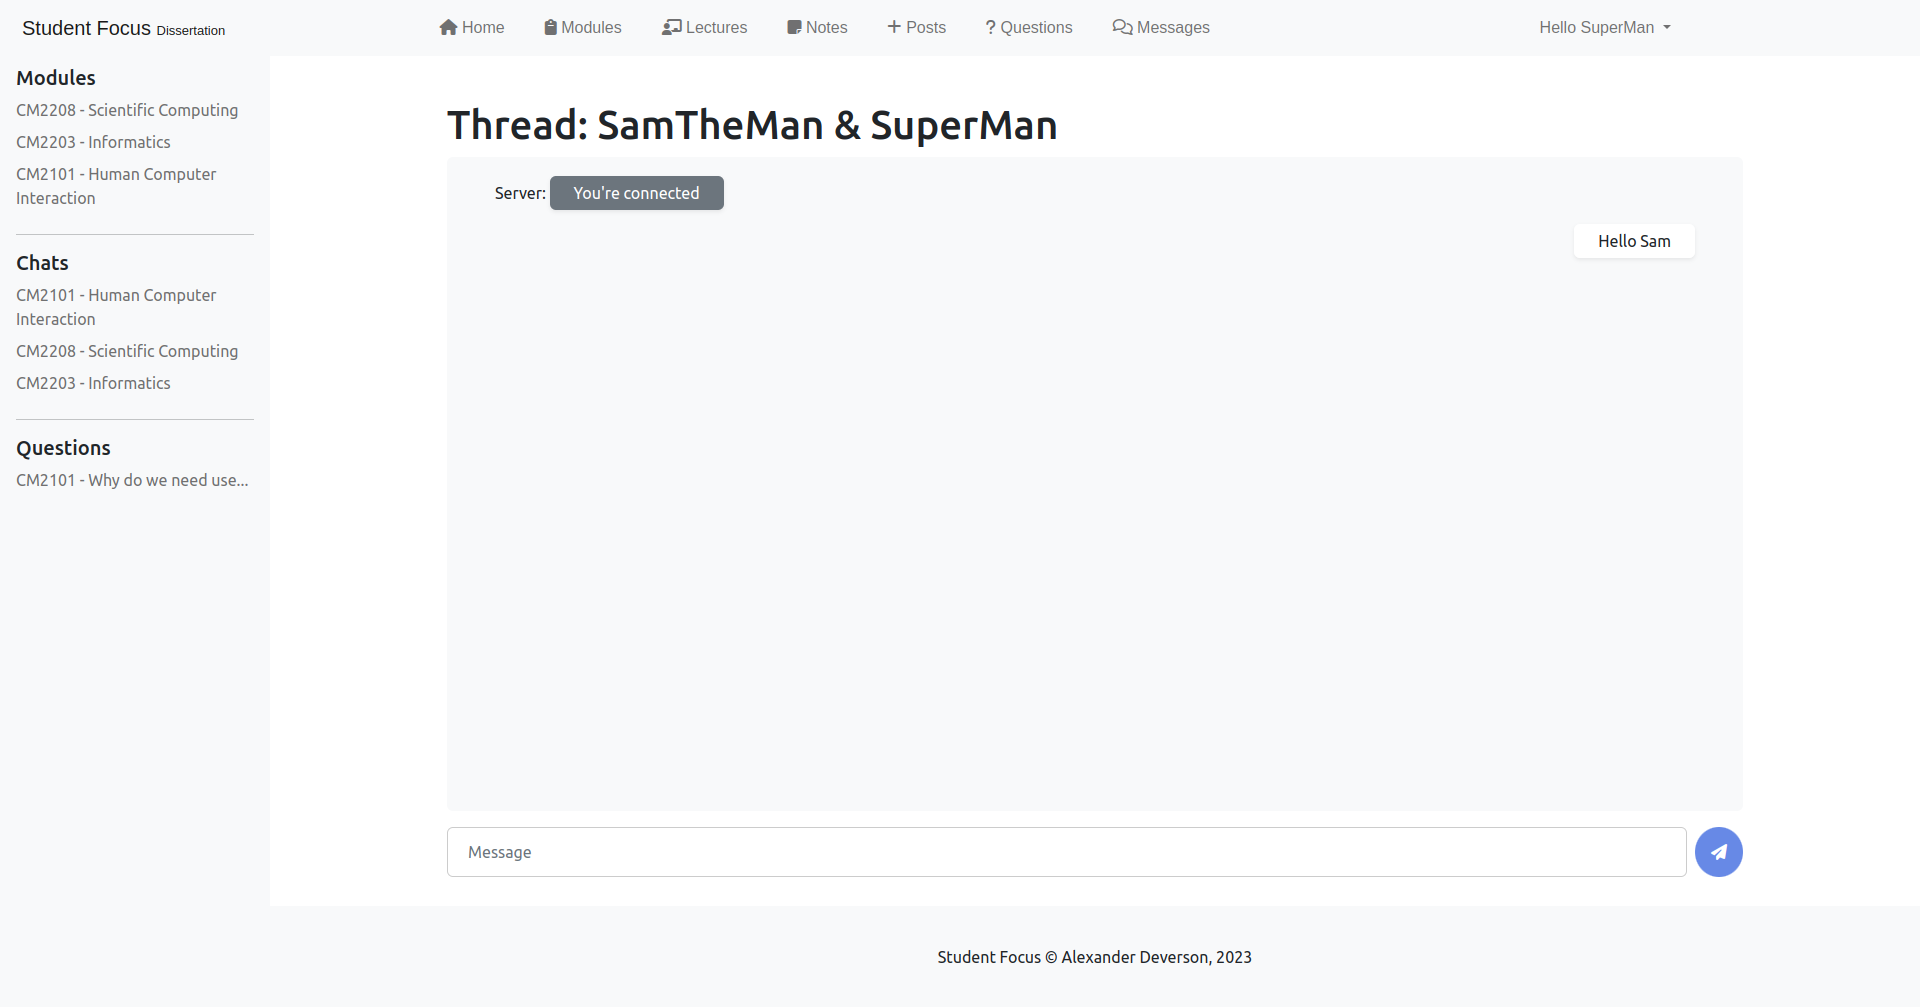
\includegraphics[scale=0.20]{images/application/24 - sending_sam_a_message.png}

New message thread



\includegraphics[scale=0.40]{images/application/65 - url_new_message_thread.png}

The URL when a new thread is started

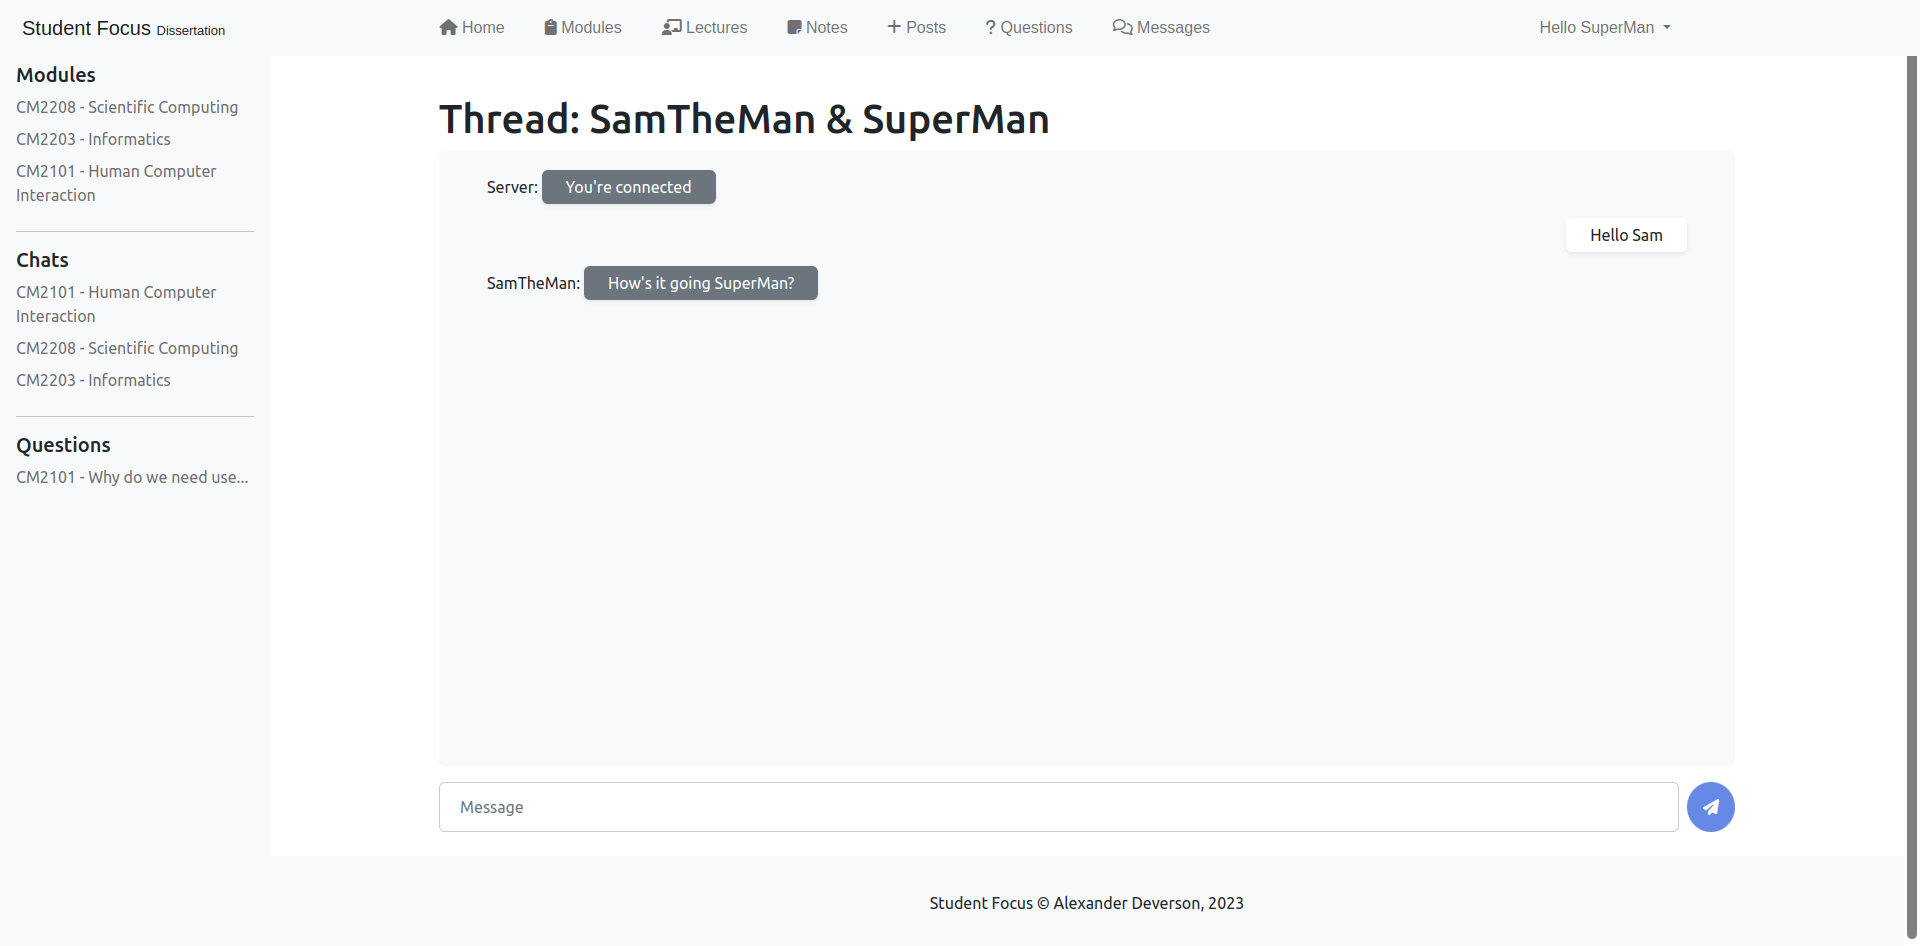
\includegraphics[scale=0.20]{images/application/25 - message_from Sam.png}

New message from a friend

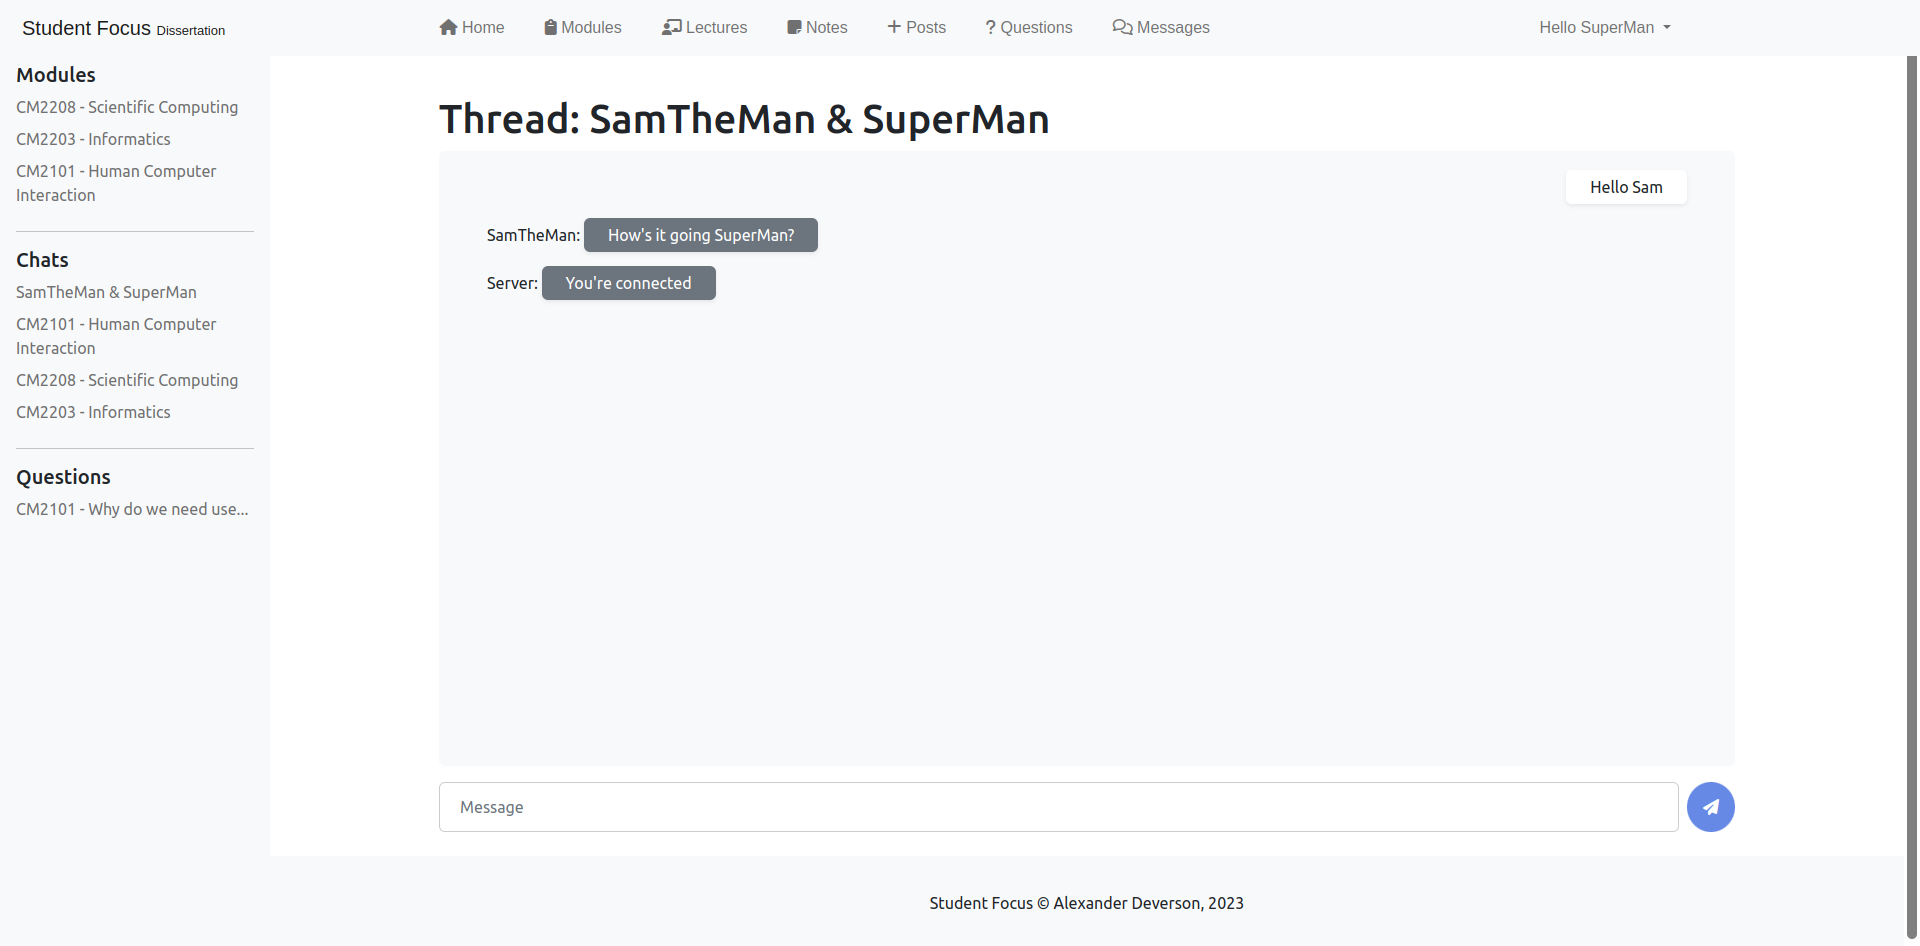
\includegraphics[scale=0.20]{images/application/26 - message_thread_on_refresh.png}

After refreshing the message thread page

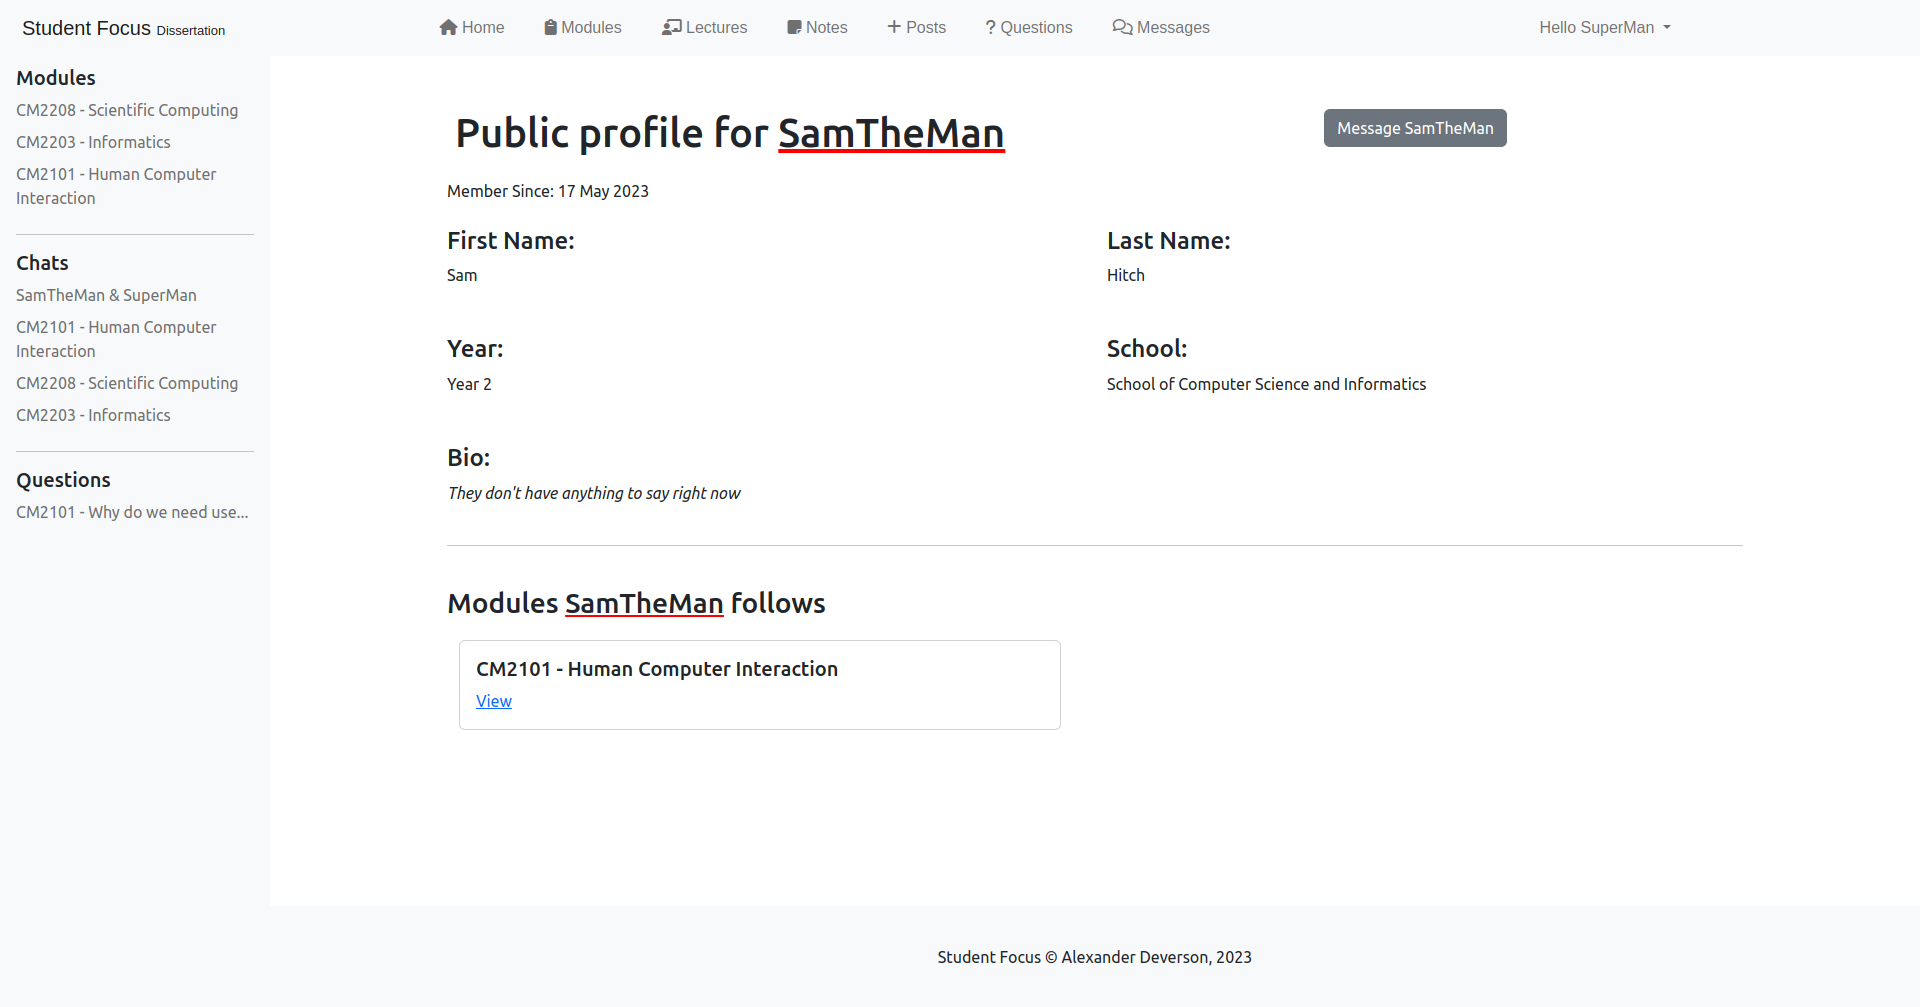
\includegraphics[scale=0.20]{images/application/27 - sams_profile.png}

Viewing another user's profile page

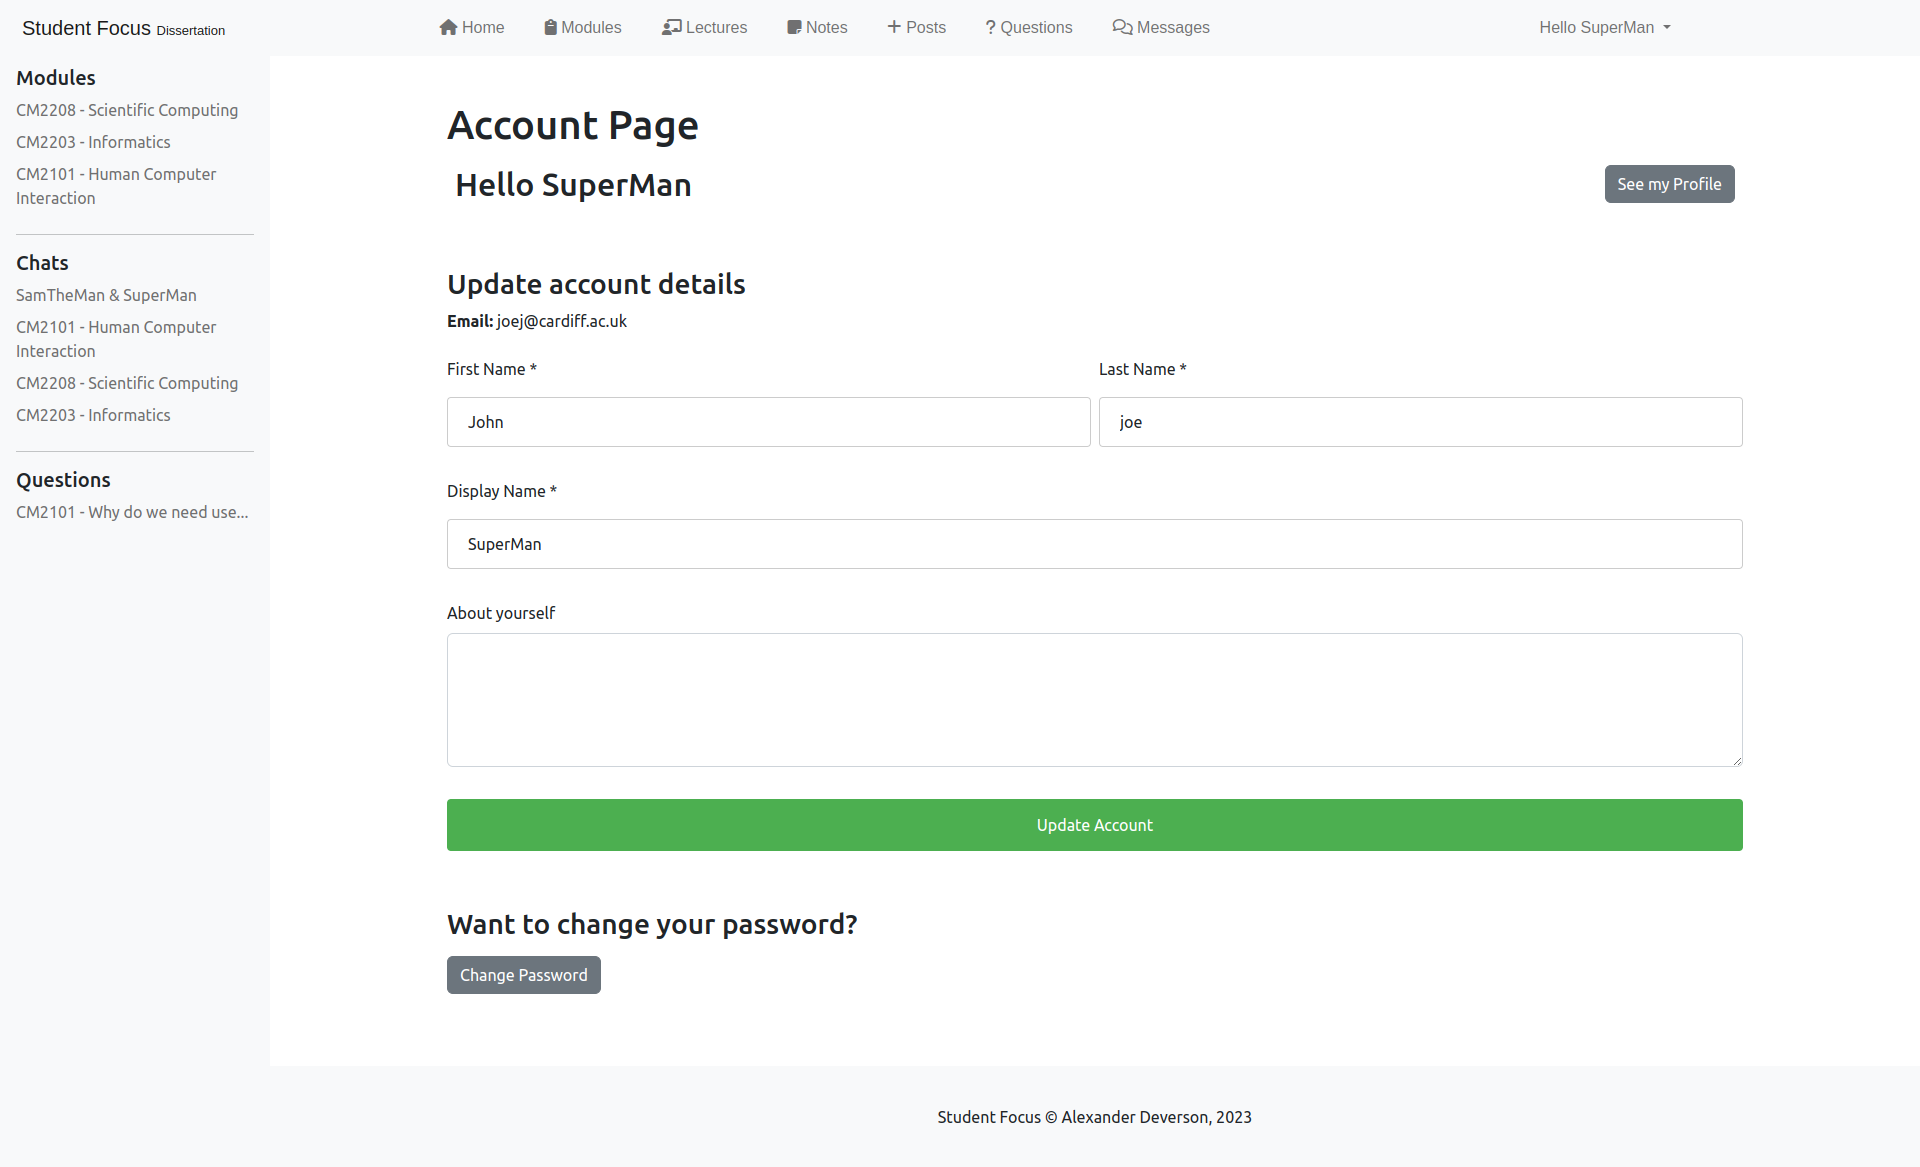
\includegraphics[scale=0.20]{images/application/28 - user_account_page.png}

The account page of the logged in user

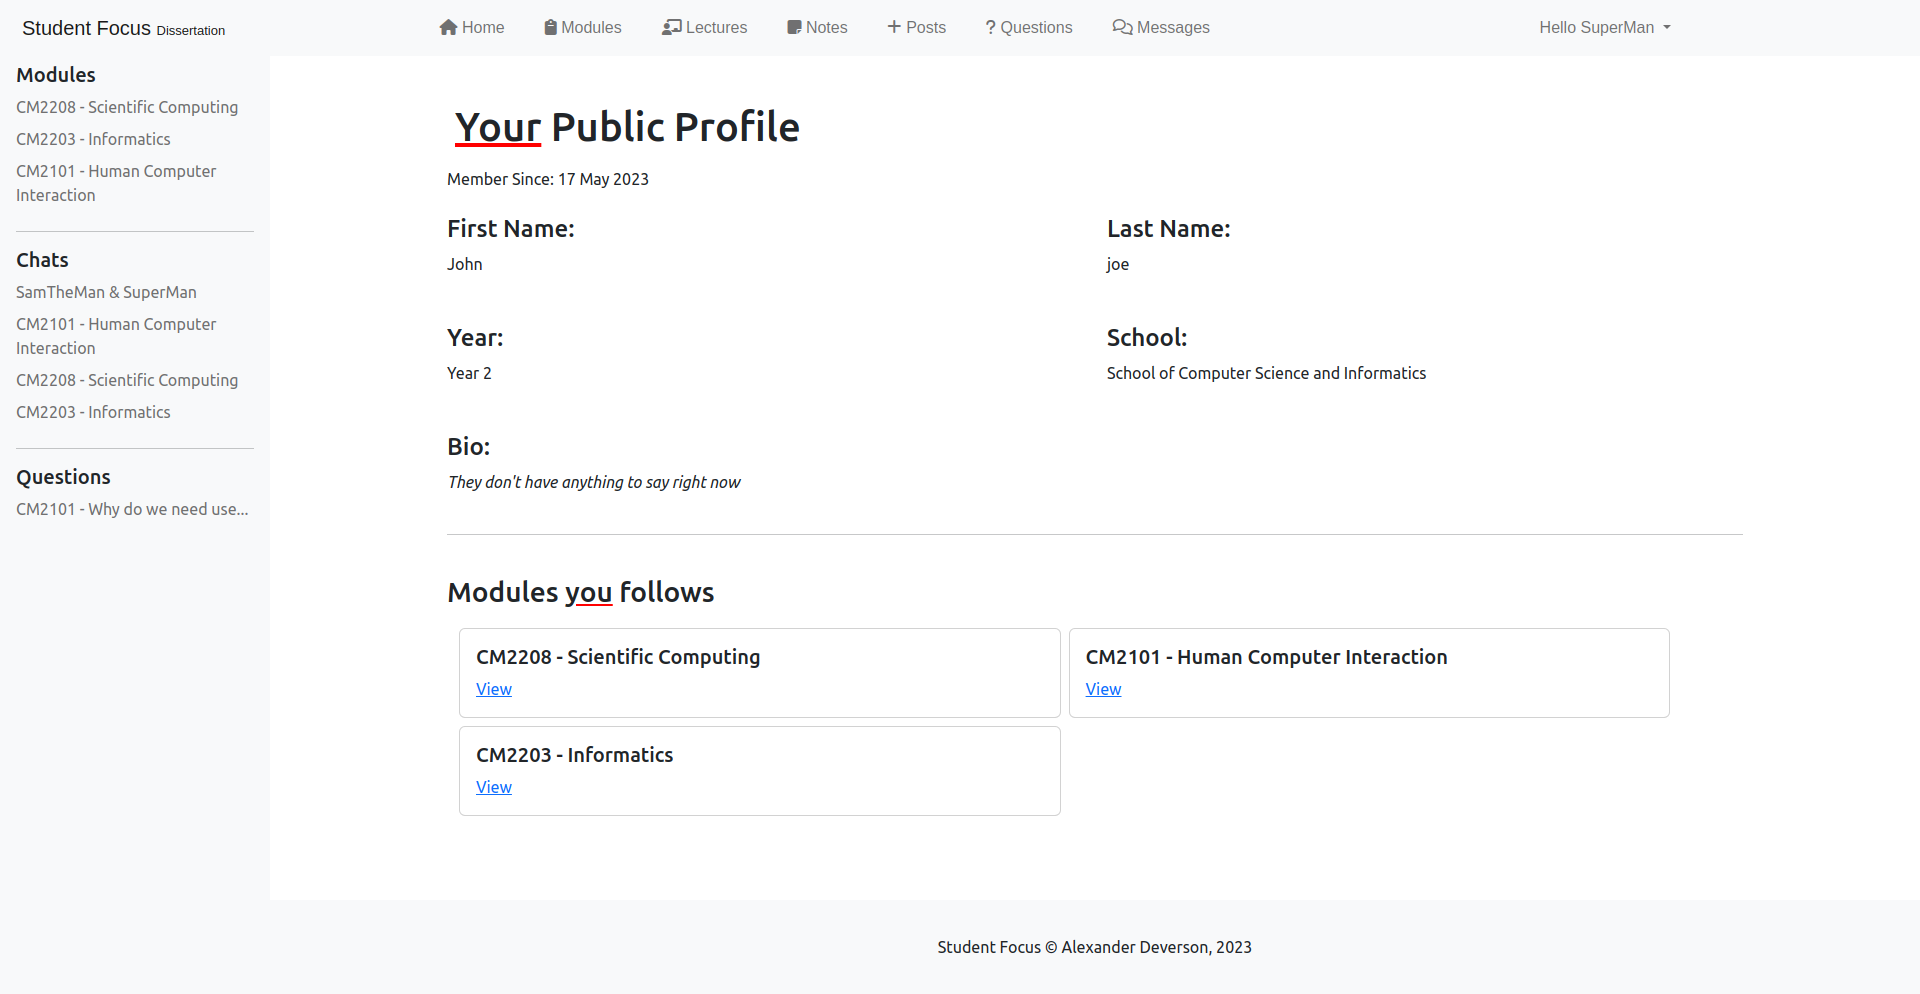
\includegraphics[scale=0.20]{images/application/29 - users_profile.png}

The account page of the logged in user

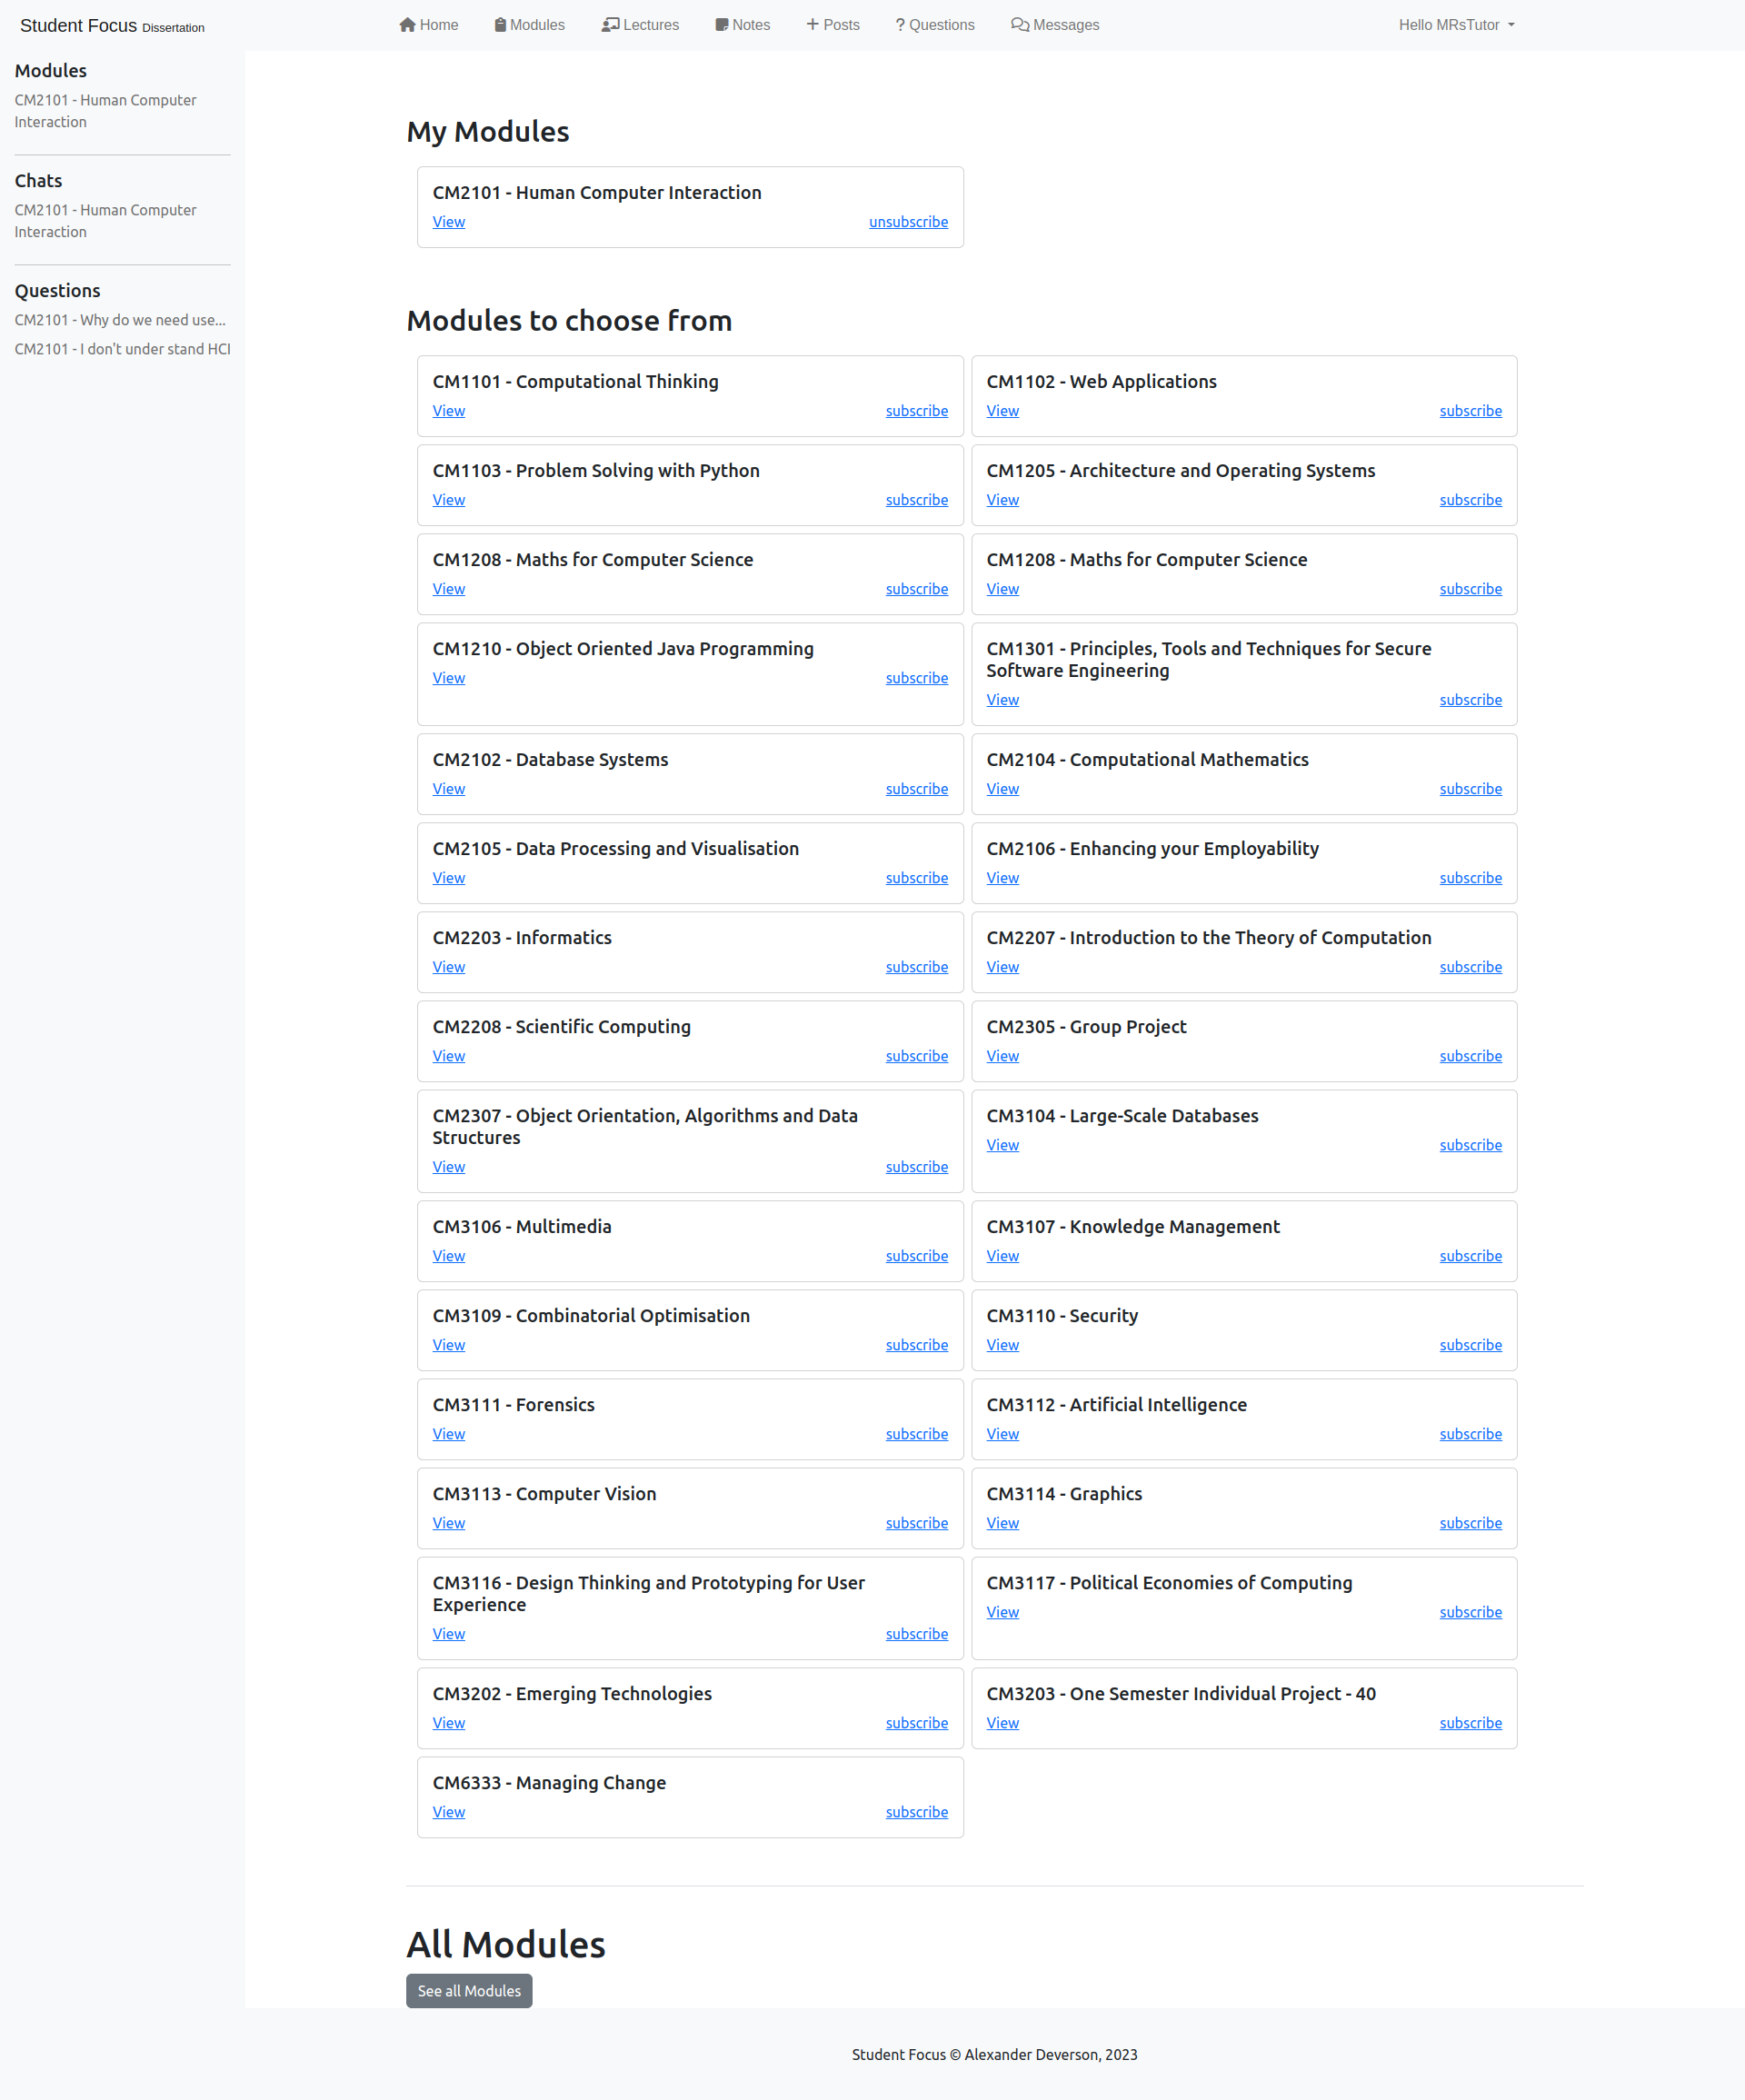
\includegraphics[scale=0.20]{images/application/30 - tutor_module_selection.png}

What a tutor sees when selecting a module

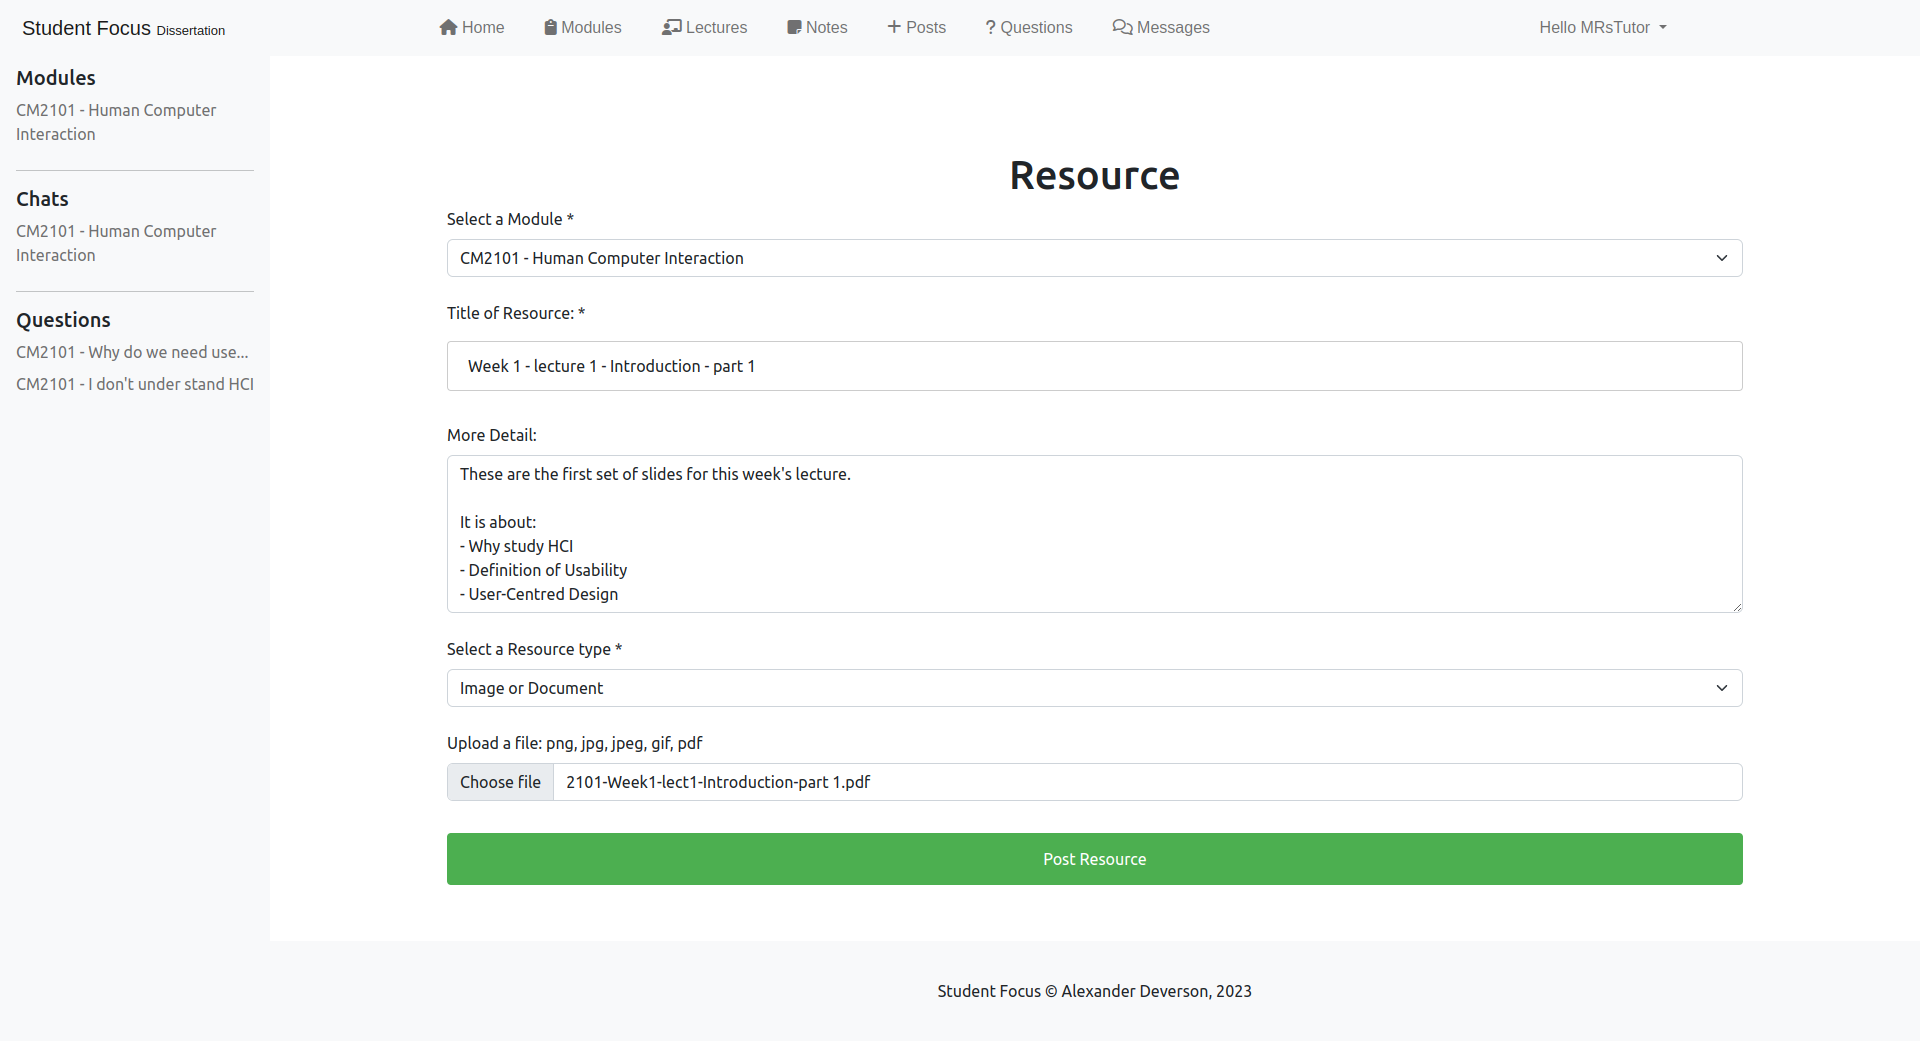
\includegraphics[scale=0.20]{images/application/31 - tutor_add_resource.png}

Adding a resource to the tutor resources

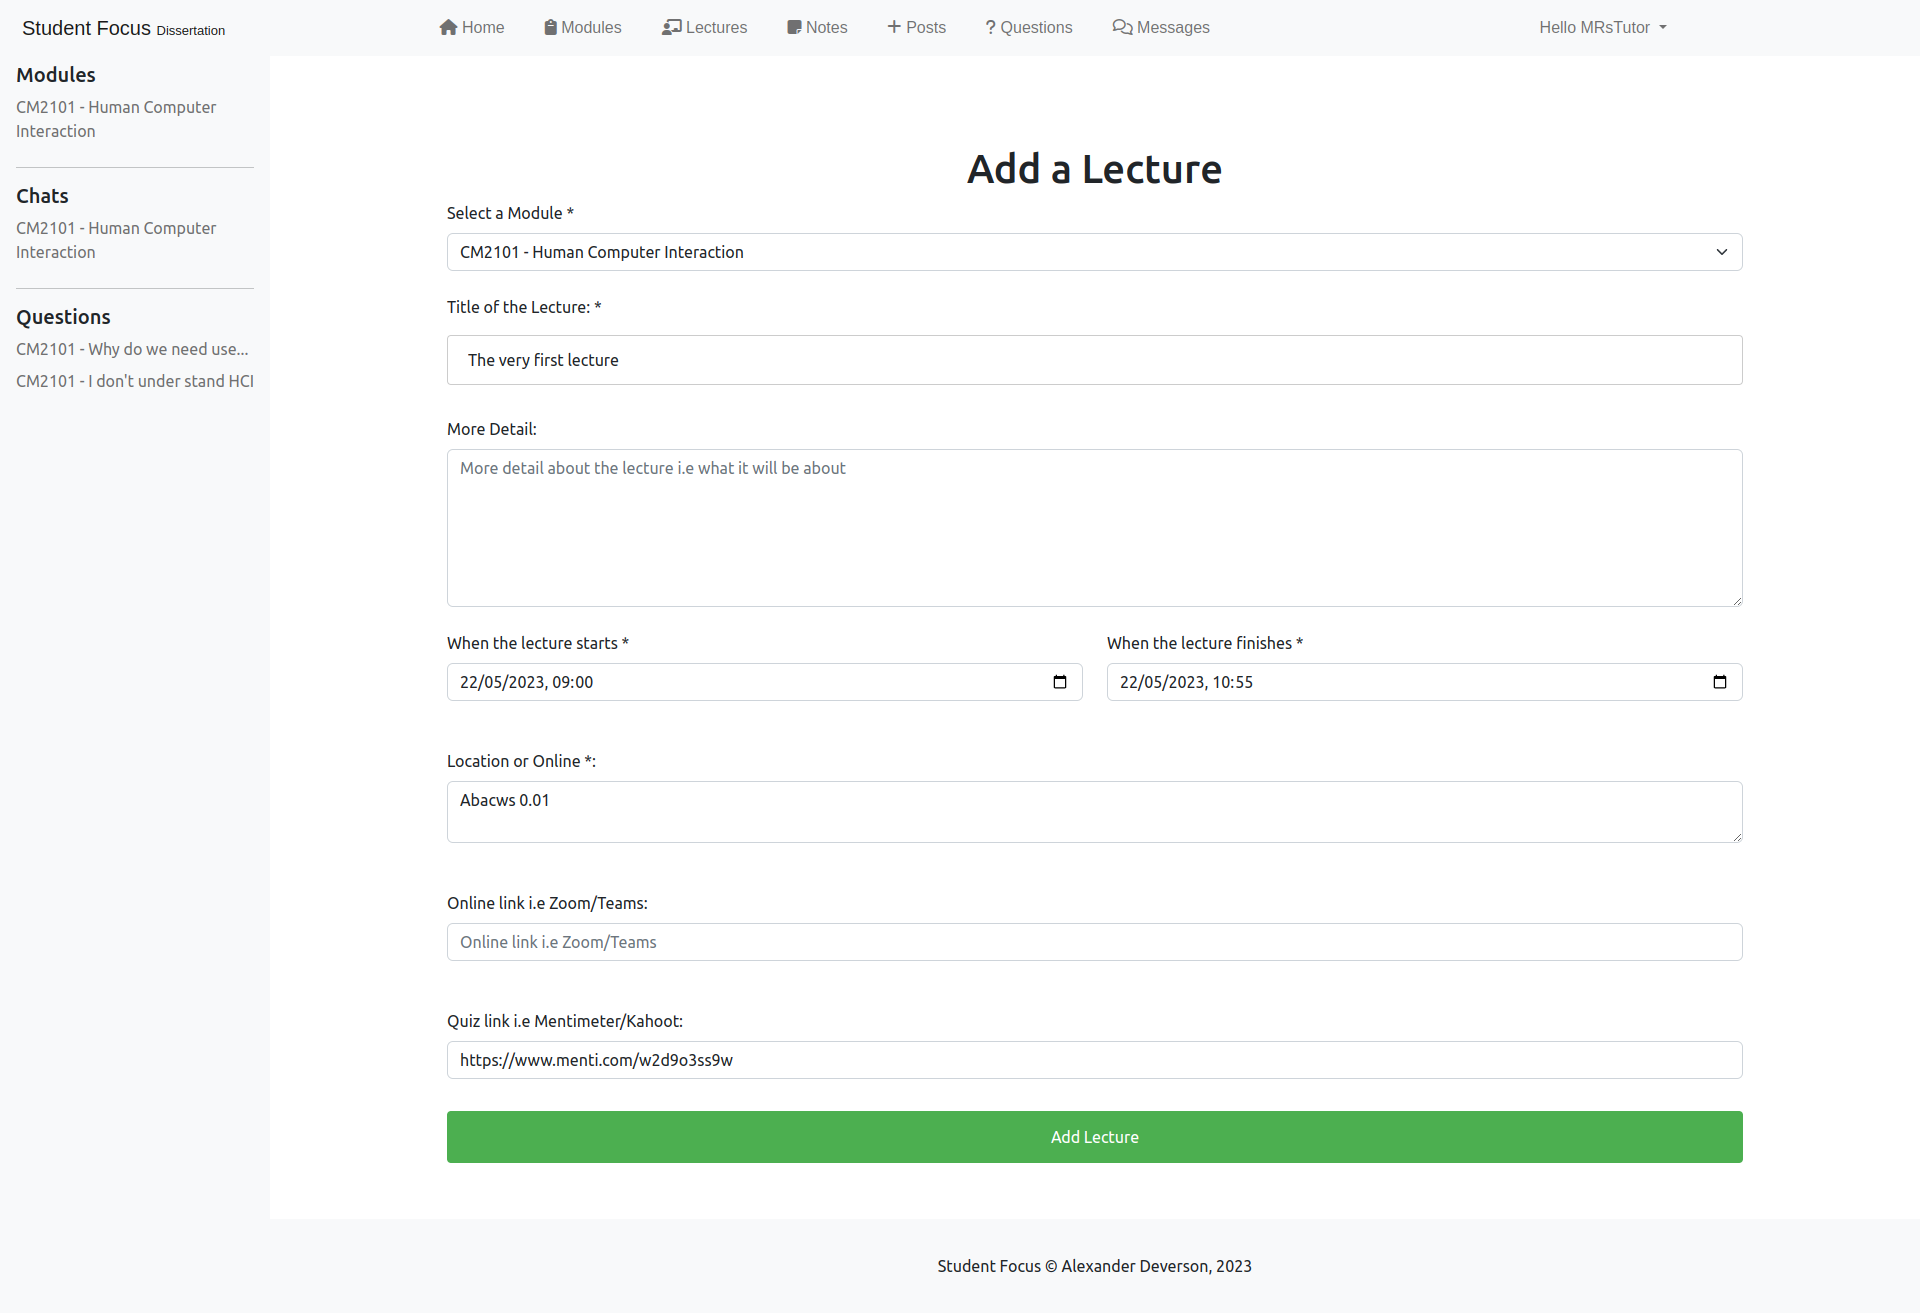
\includegraphics[scale=0.20]{images/application/32 - add_lecture.png}

Adding a lecture

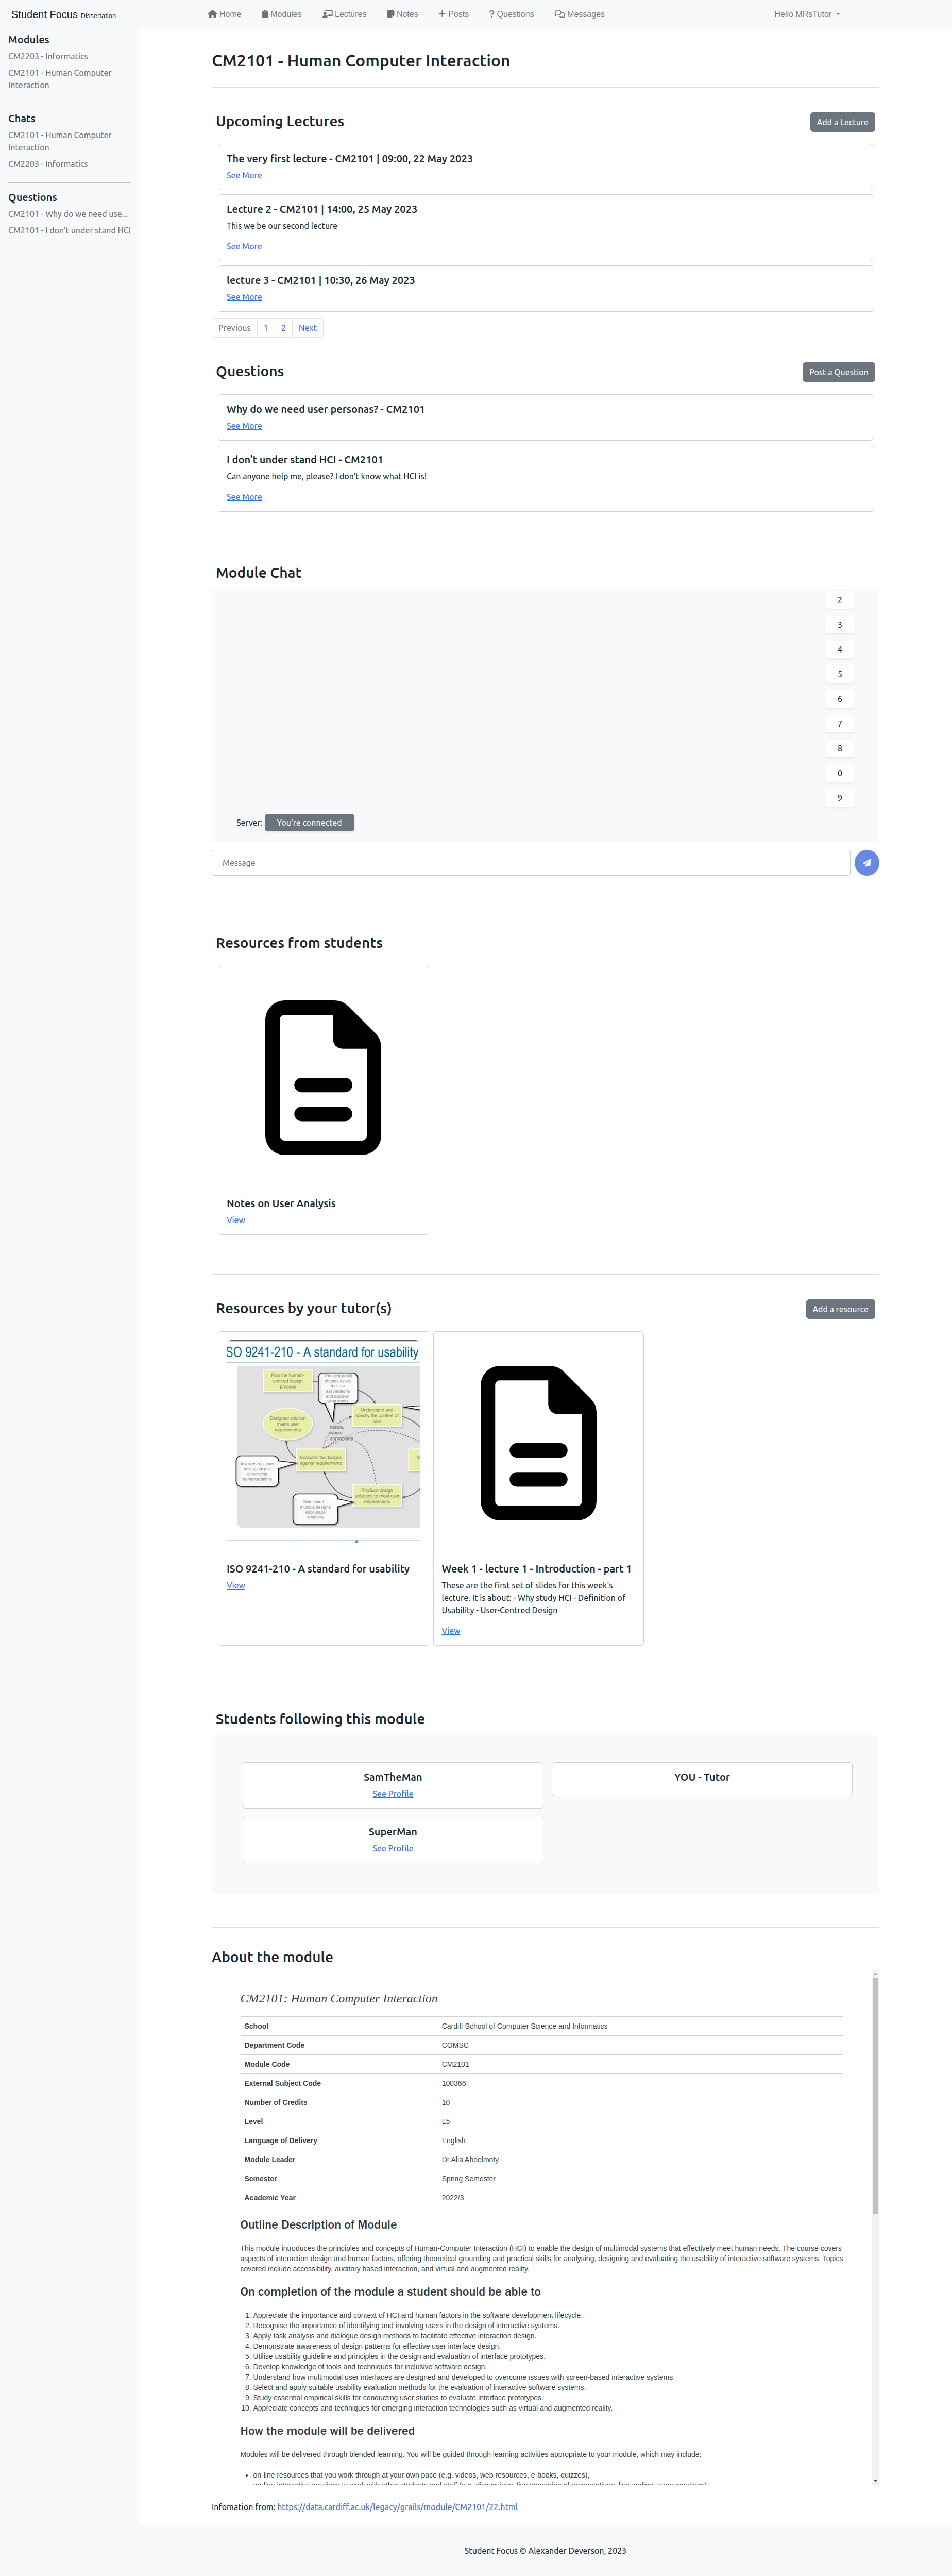
\includegraphics[scale=0.12]{images/application/33 - module_page_populated.png}

Single module page after it has been populated with some content

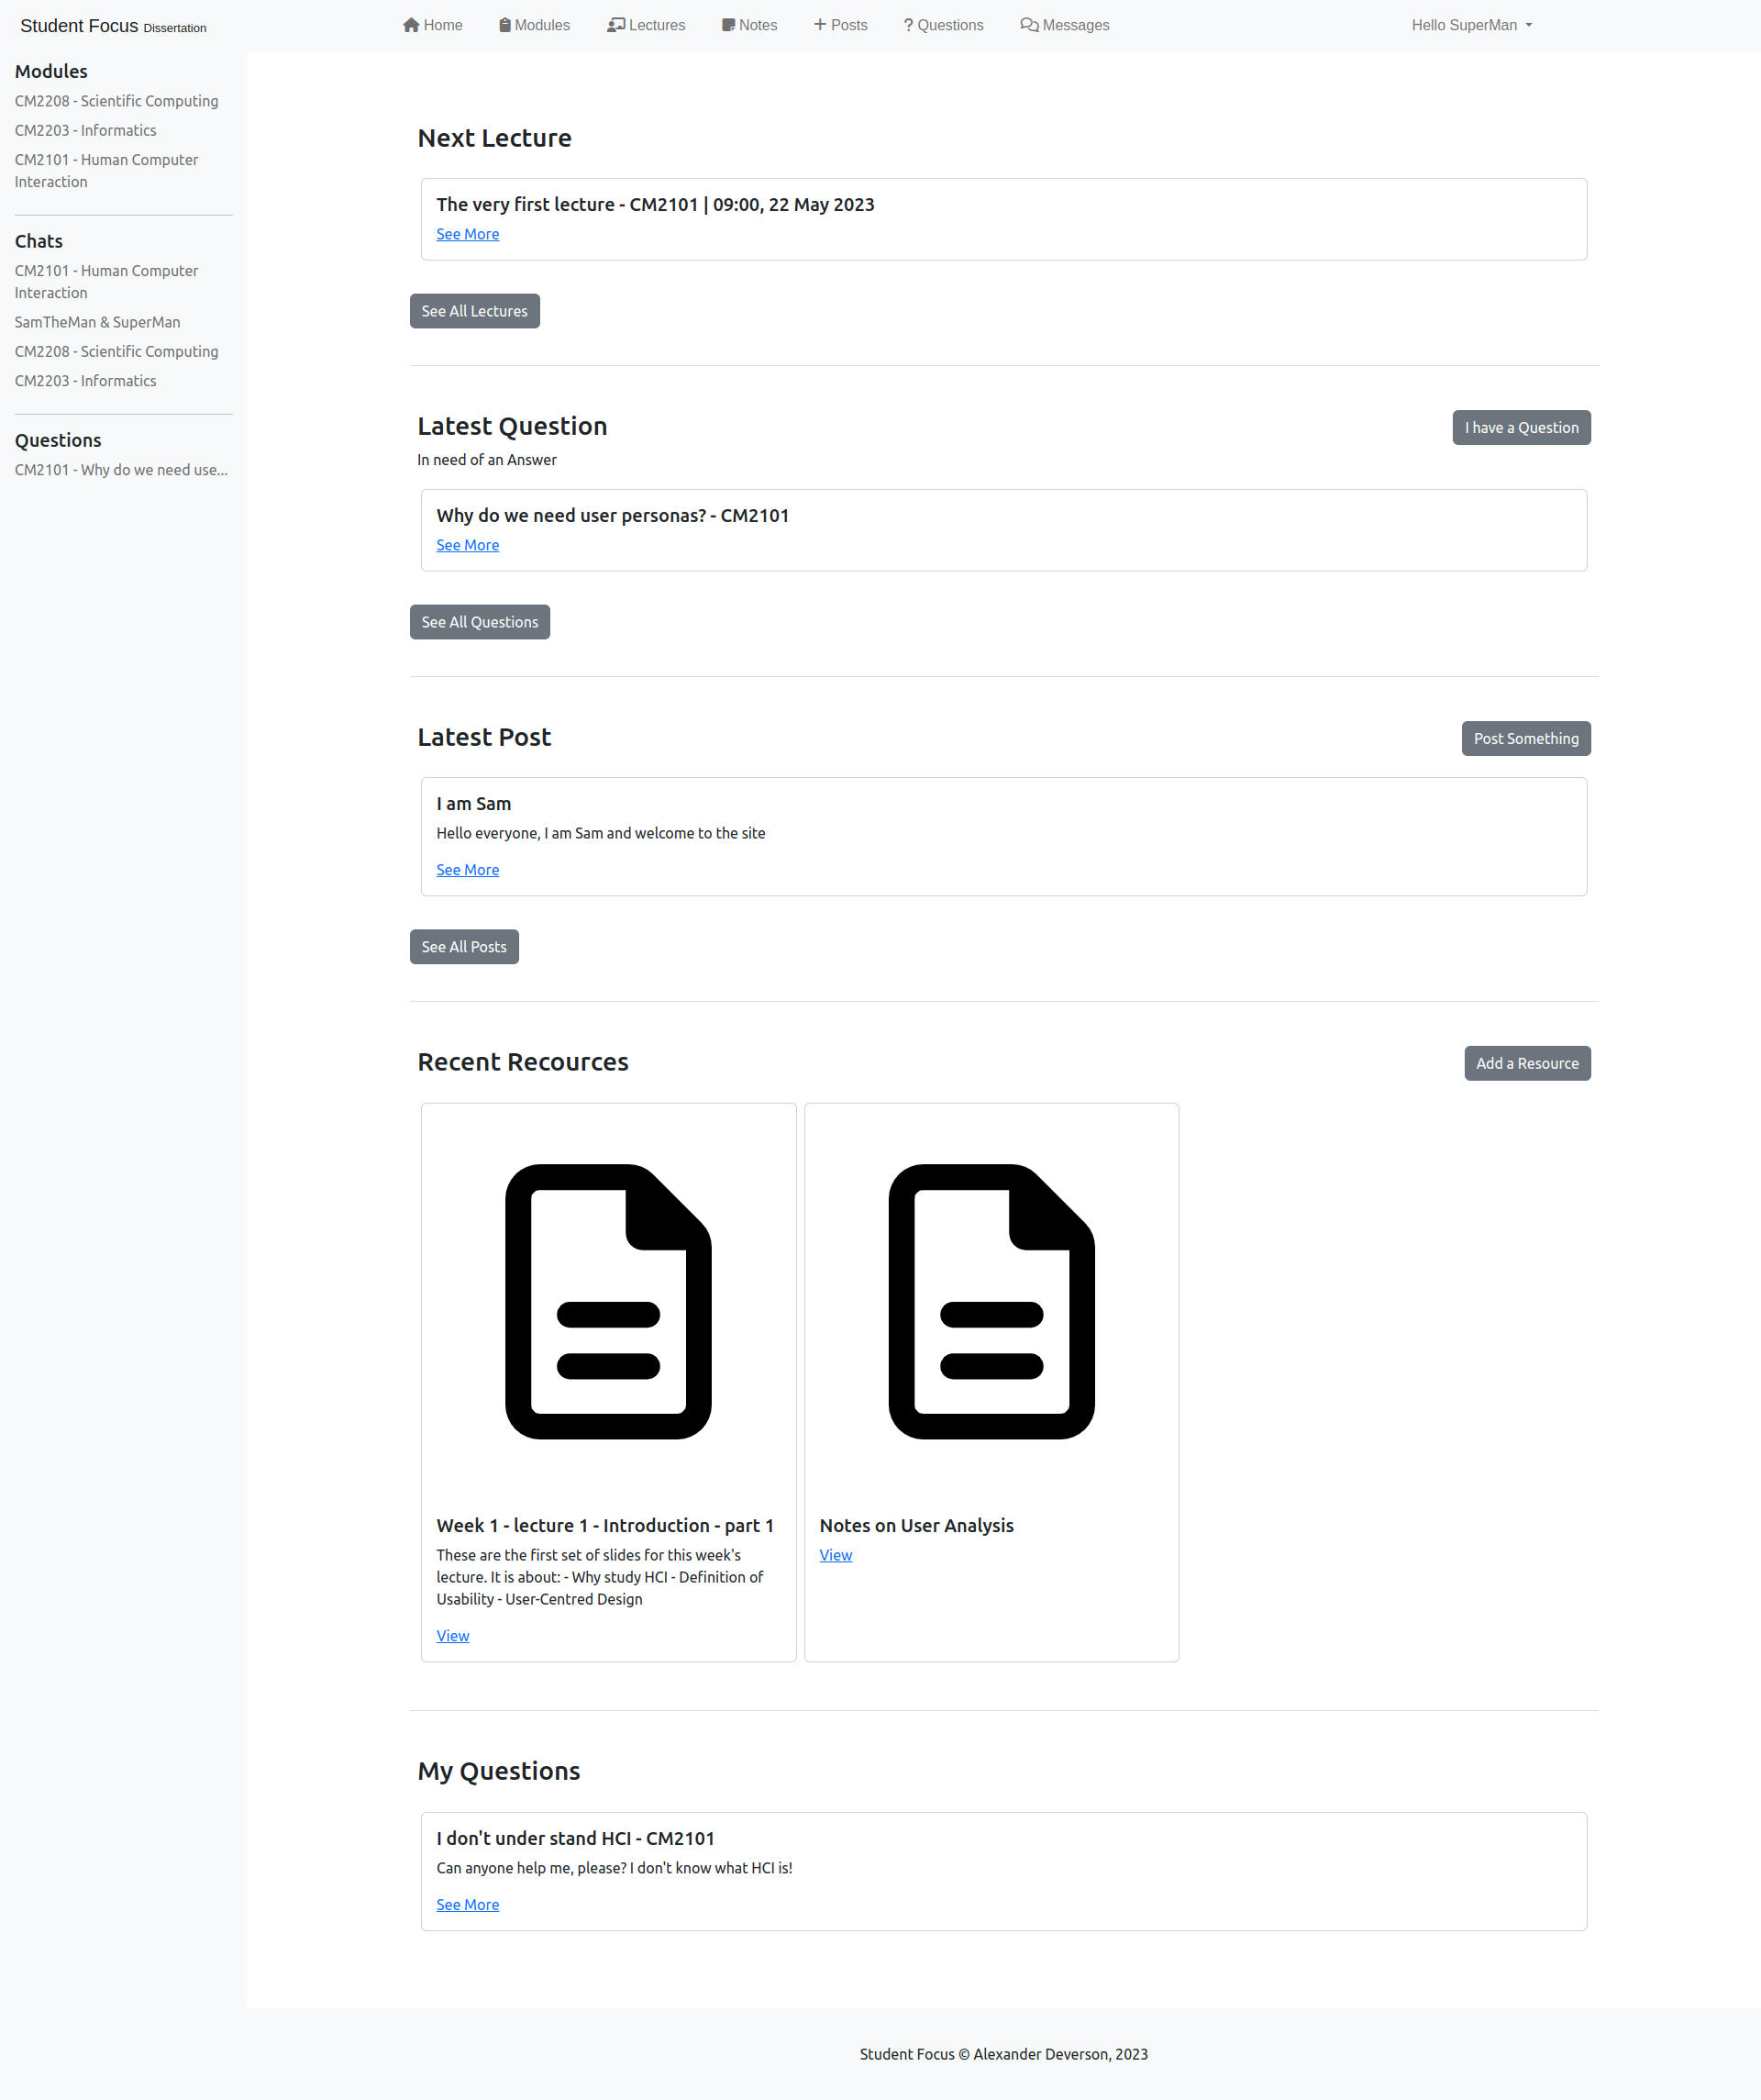
\includegraphics[scale=0.20]{images/application/34 - home_page_populated.png}

The main user home page after it has been populated with content

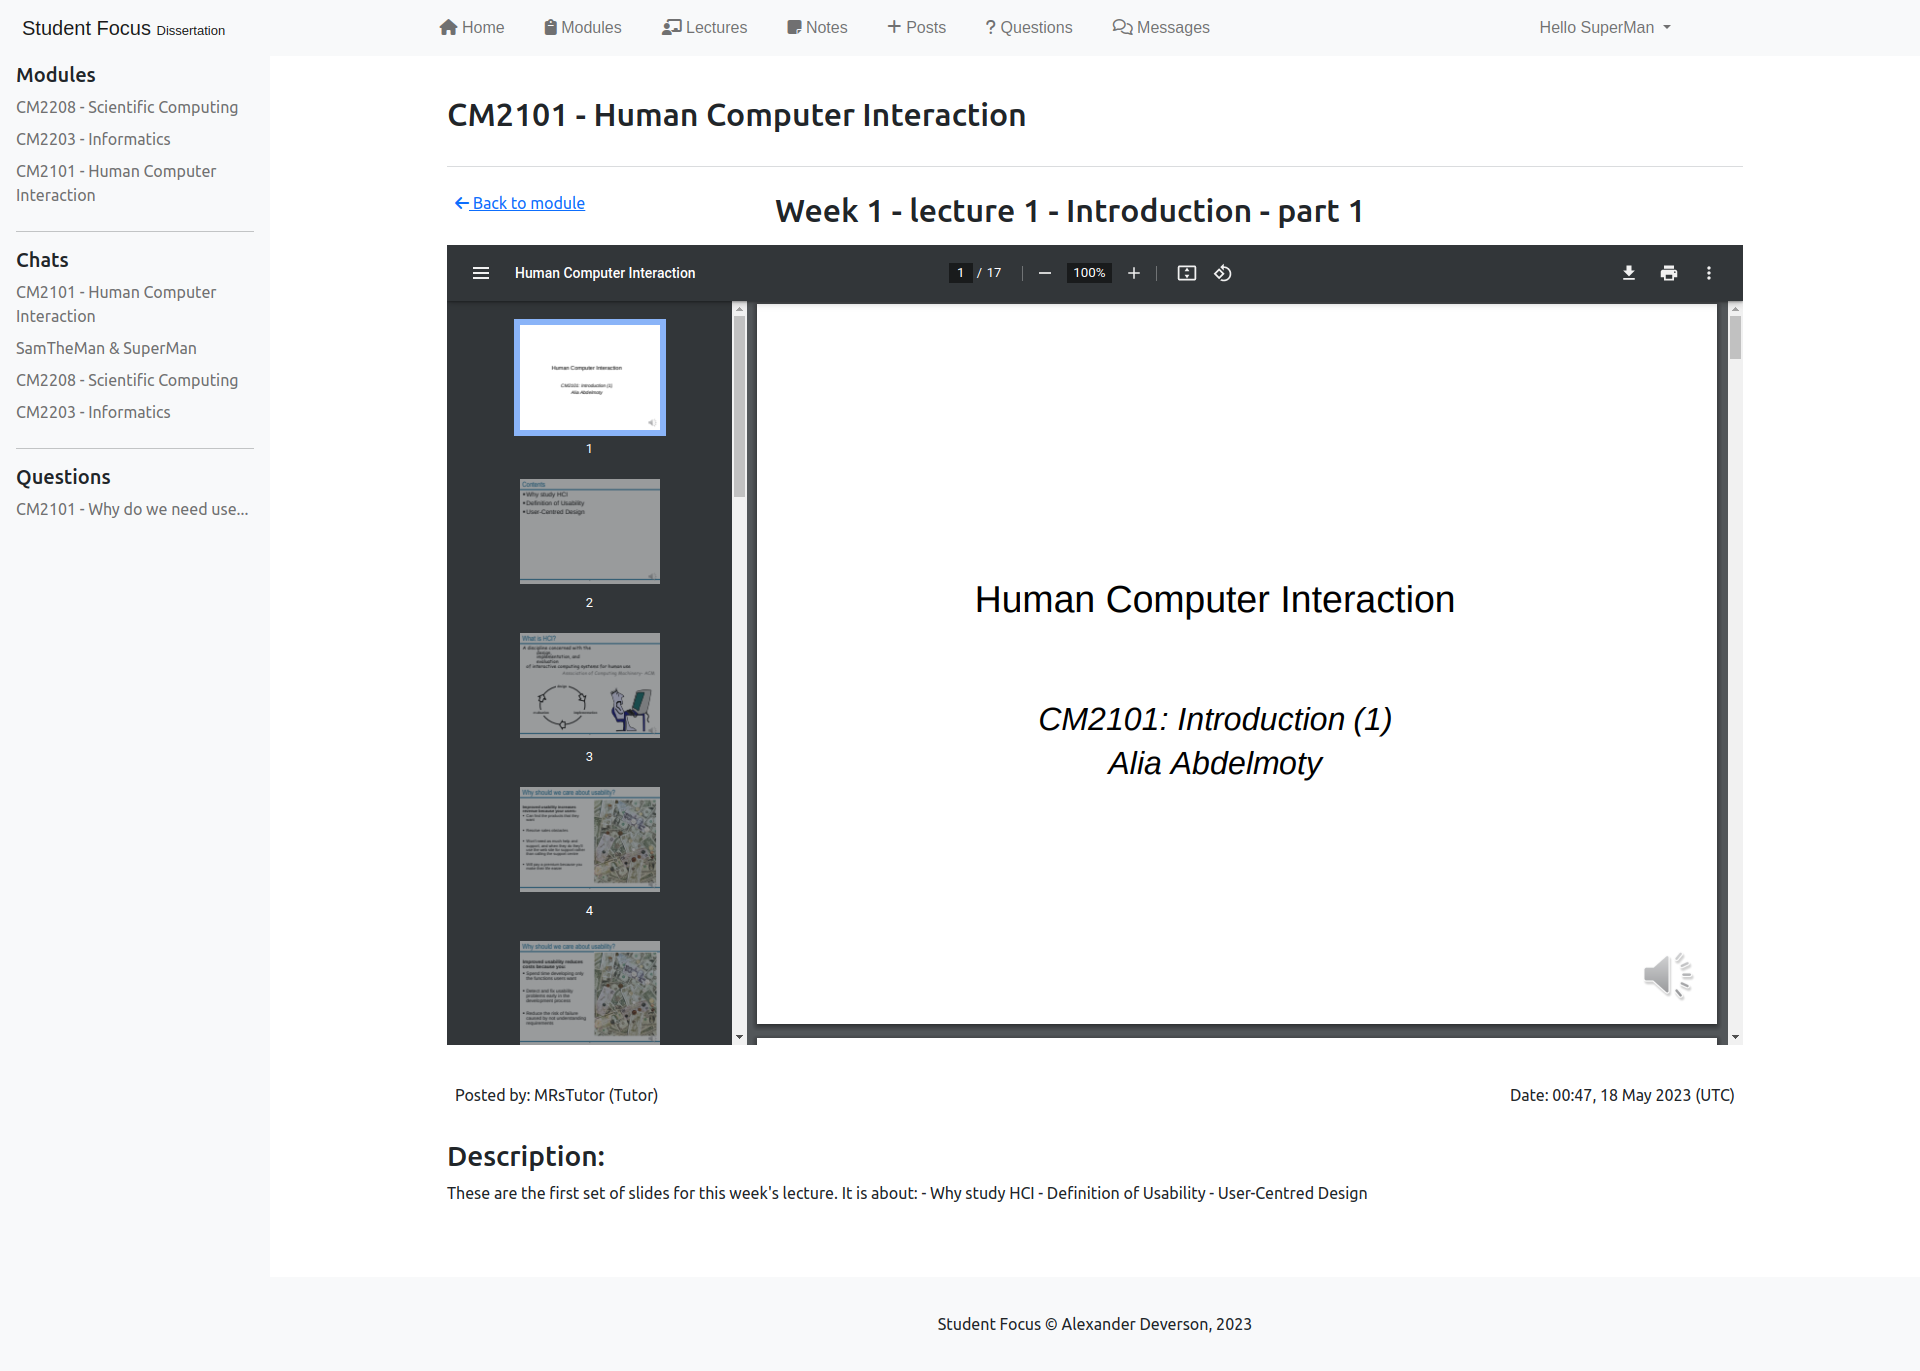
\includegraphics[scale=0.20]{images/application/35 - resource_single_view.png}

Viewing a single resource (document)

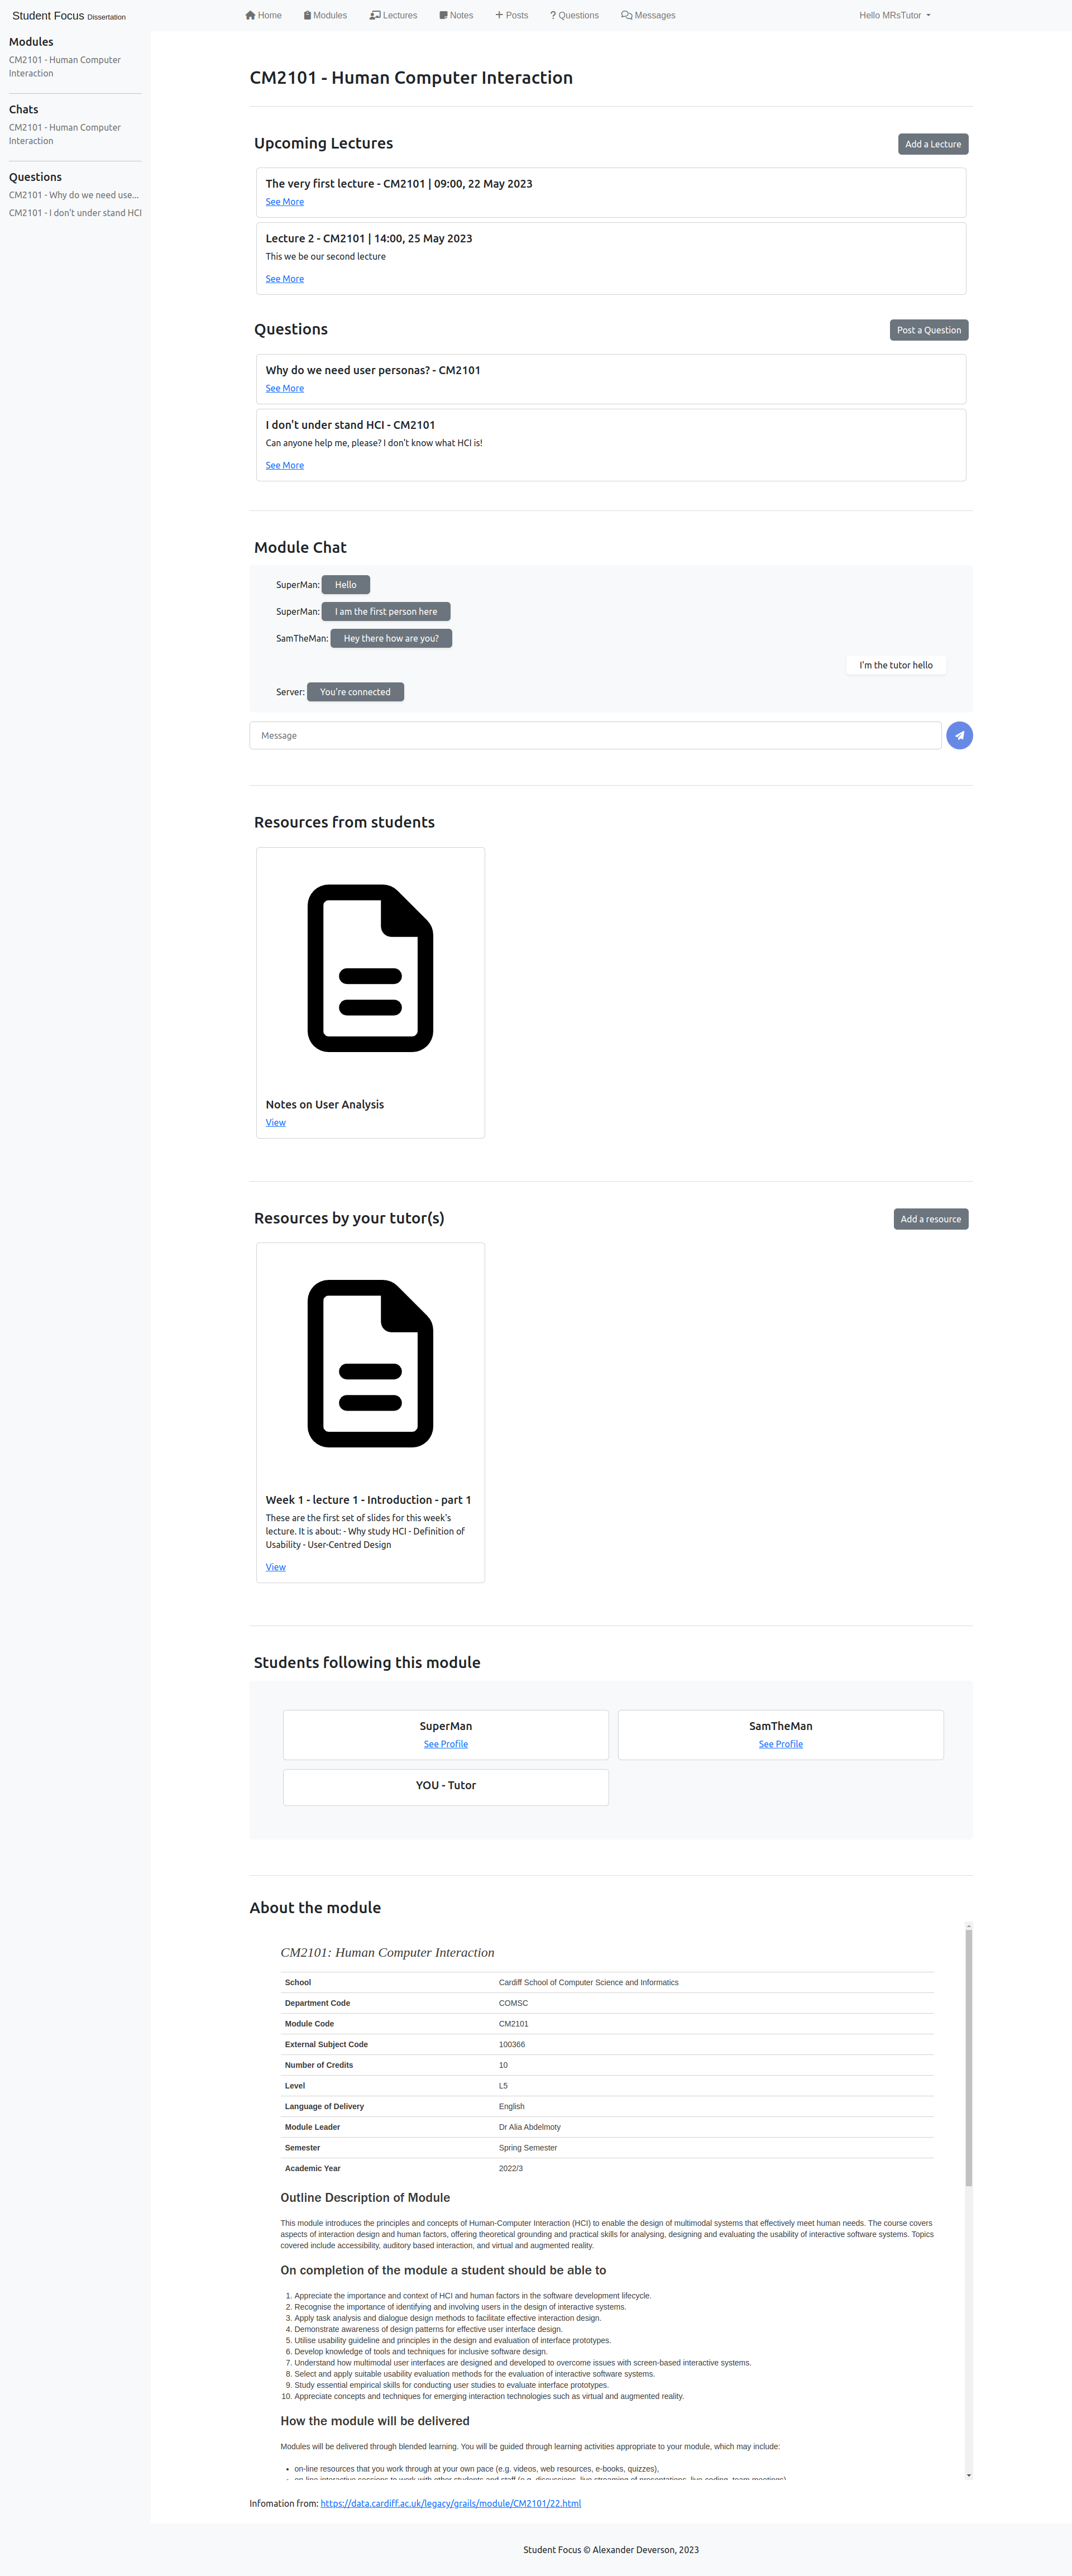
\includegraphics[scale=0.10]{images/application/36 - tutor_module_page_populated.png}

View of a single module page fully populated from the perspective of a tutor

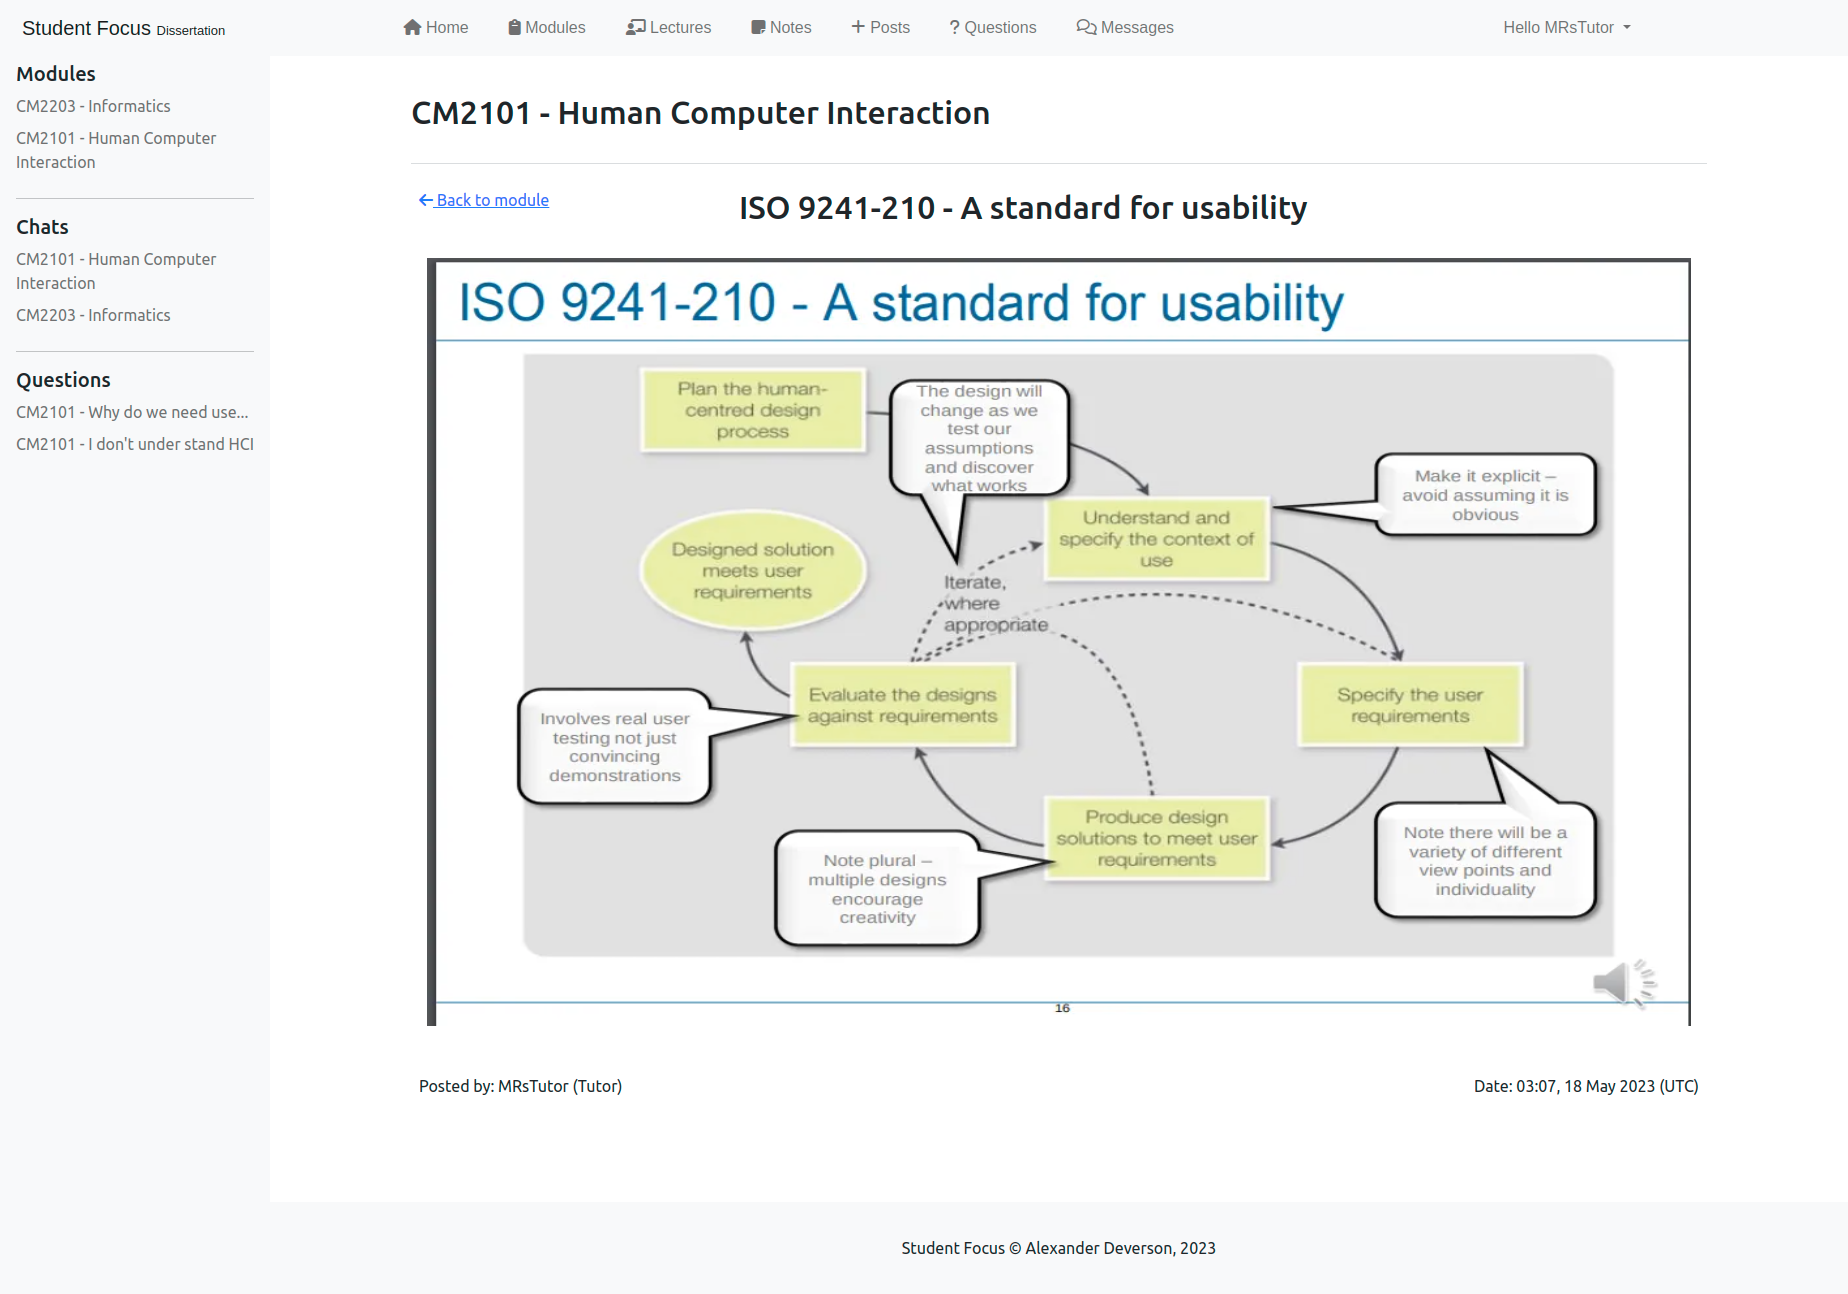
\includegraphics[scale=0.20]{images/application/66 - module_resource_single_image.png}

Viewing a single resource (image)

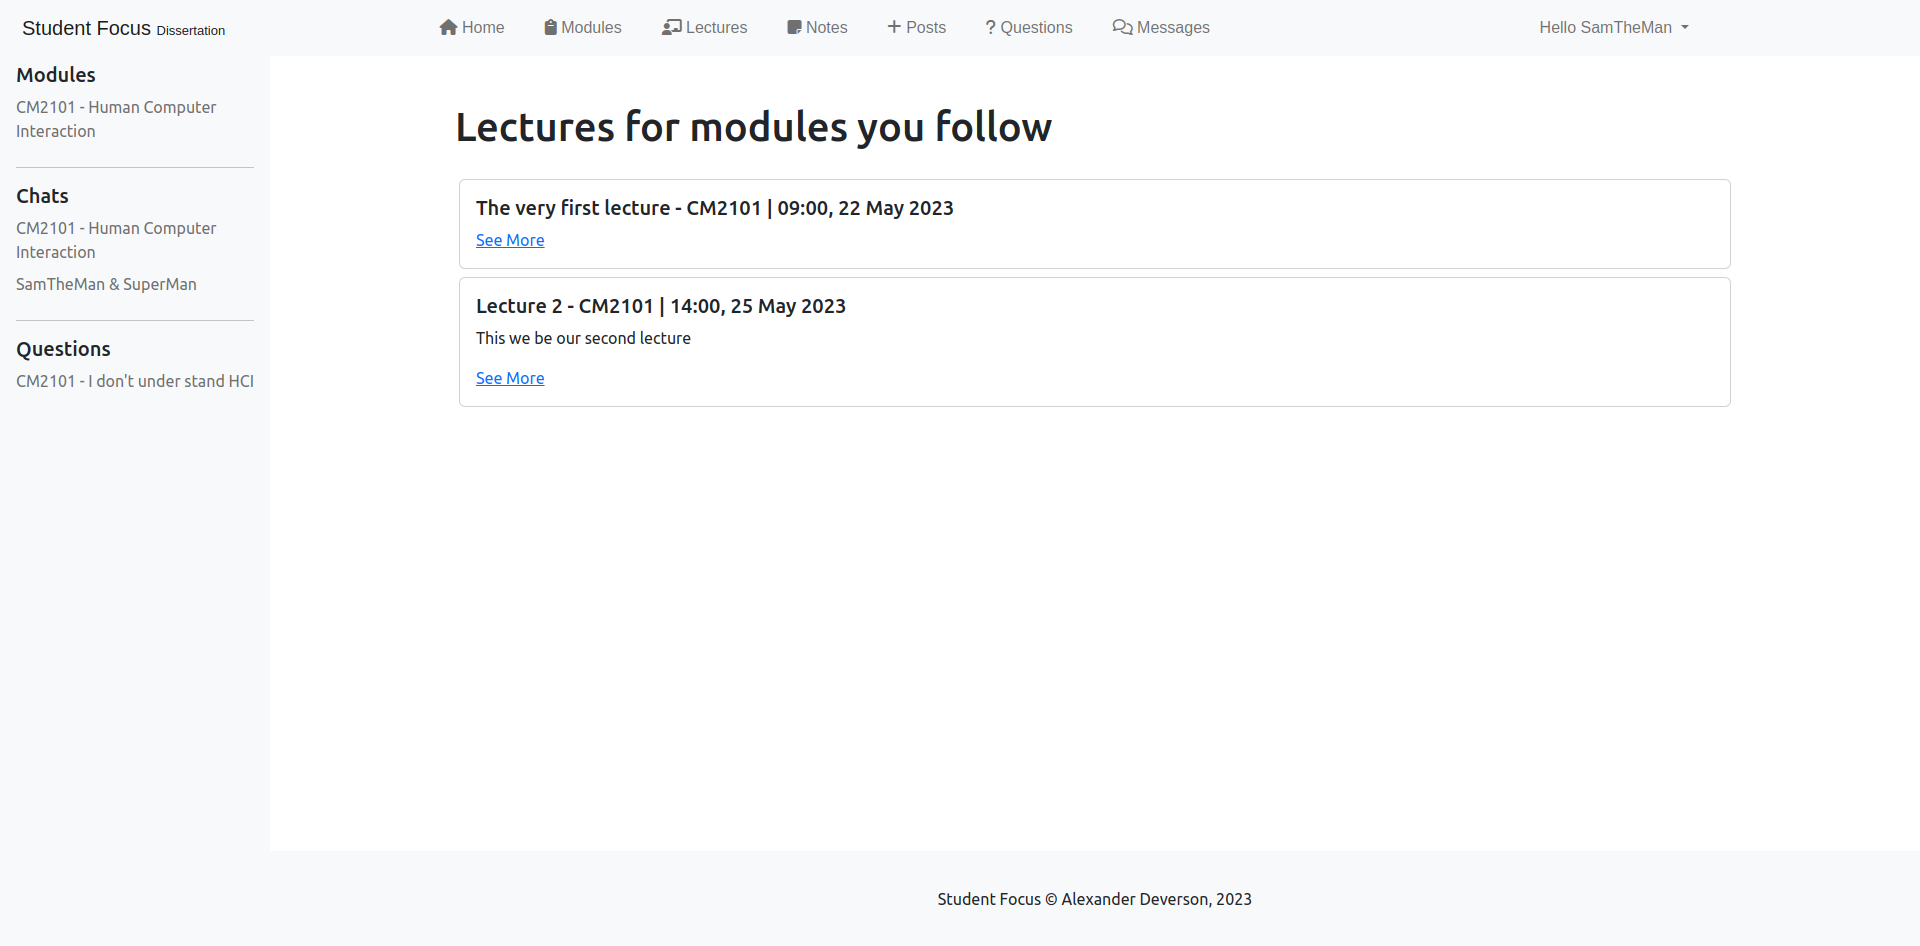
\includegraphics[scale=0.20]{images/application/37 - lecture_list.png}

A page listing all the lectures for the modules that a user has subscribed to (desktop version)

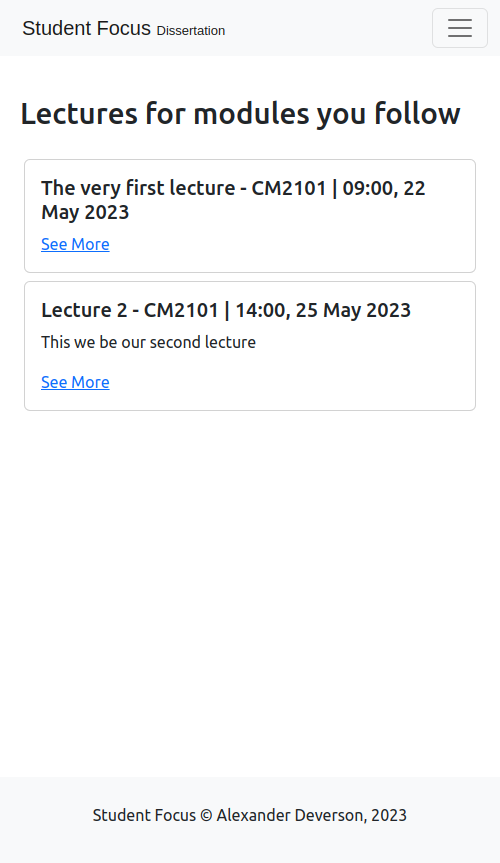
\includegraphics[scale=0.20]{images/application/40 - mobile.png}

A page listing all the lectures for the modules that a user has subscribed to (mobile version)

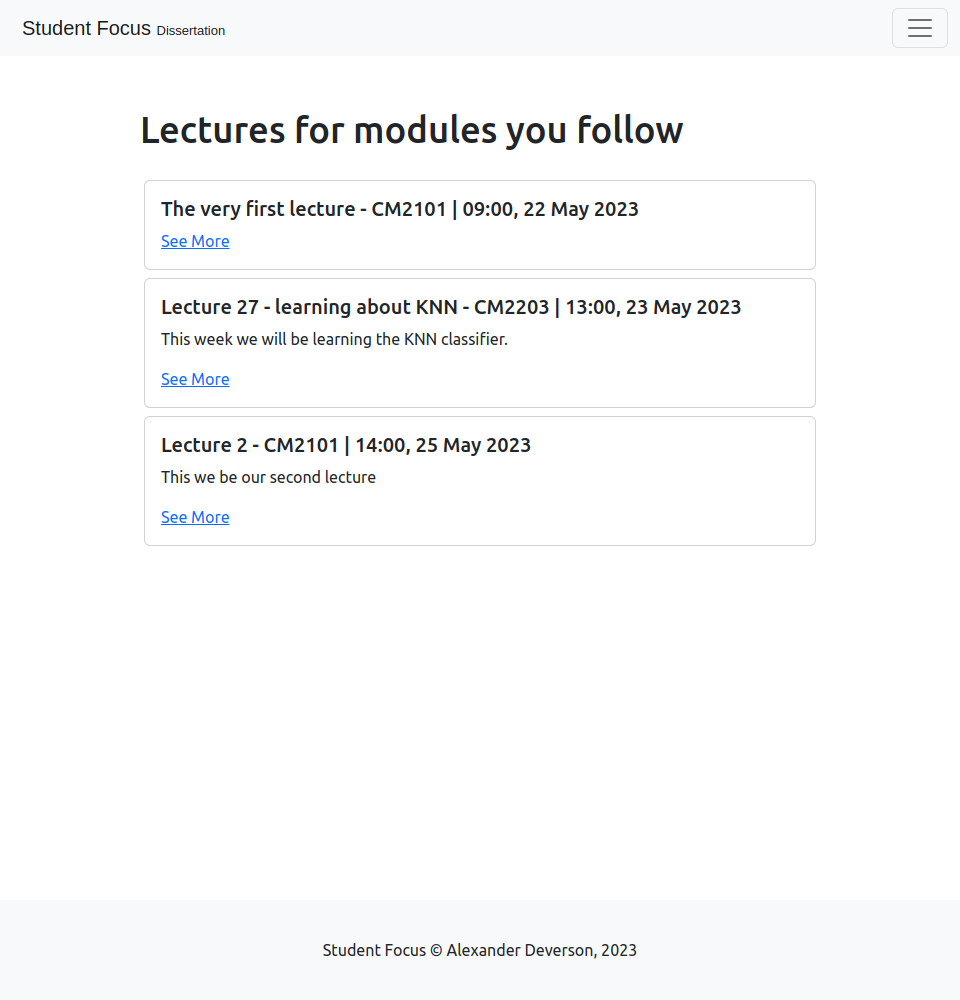
\includegraphics[scale=0.20]{images/application/38 - lecture_list_more.png}

A page listing all the lectures for the modules that a user has subscribed to (but from a user with more modules and mobile version)

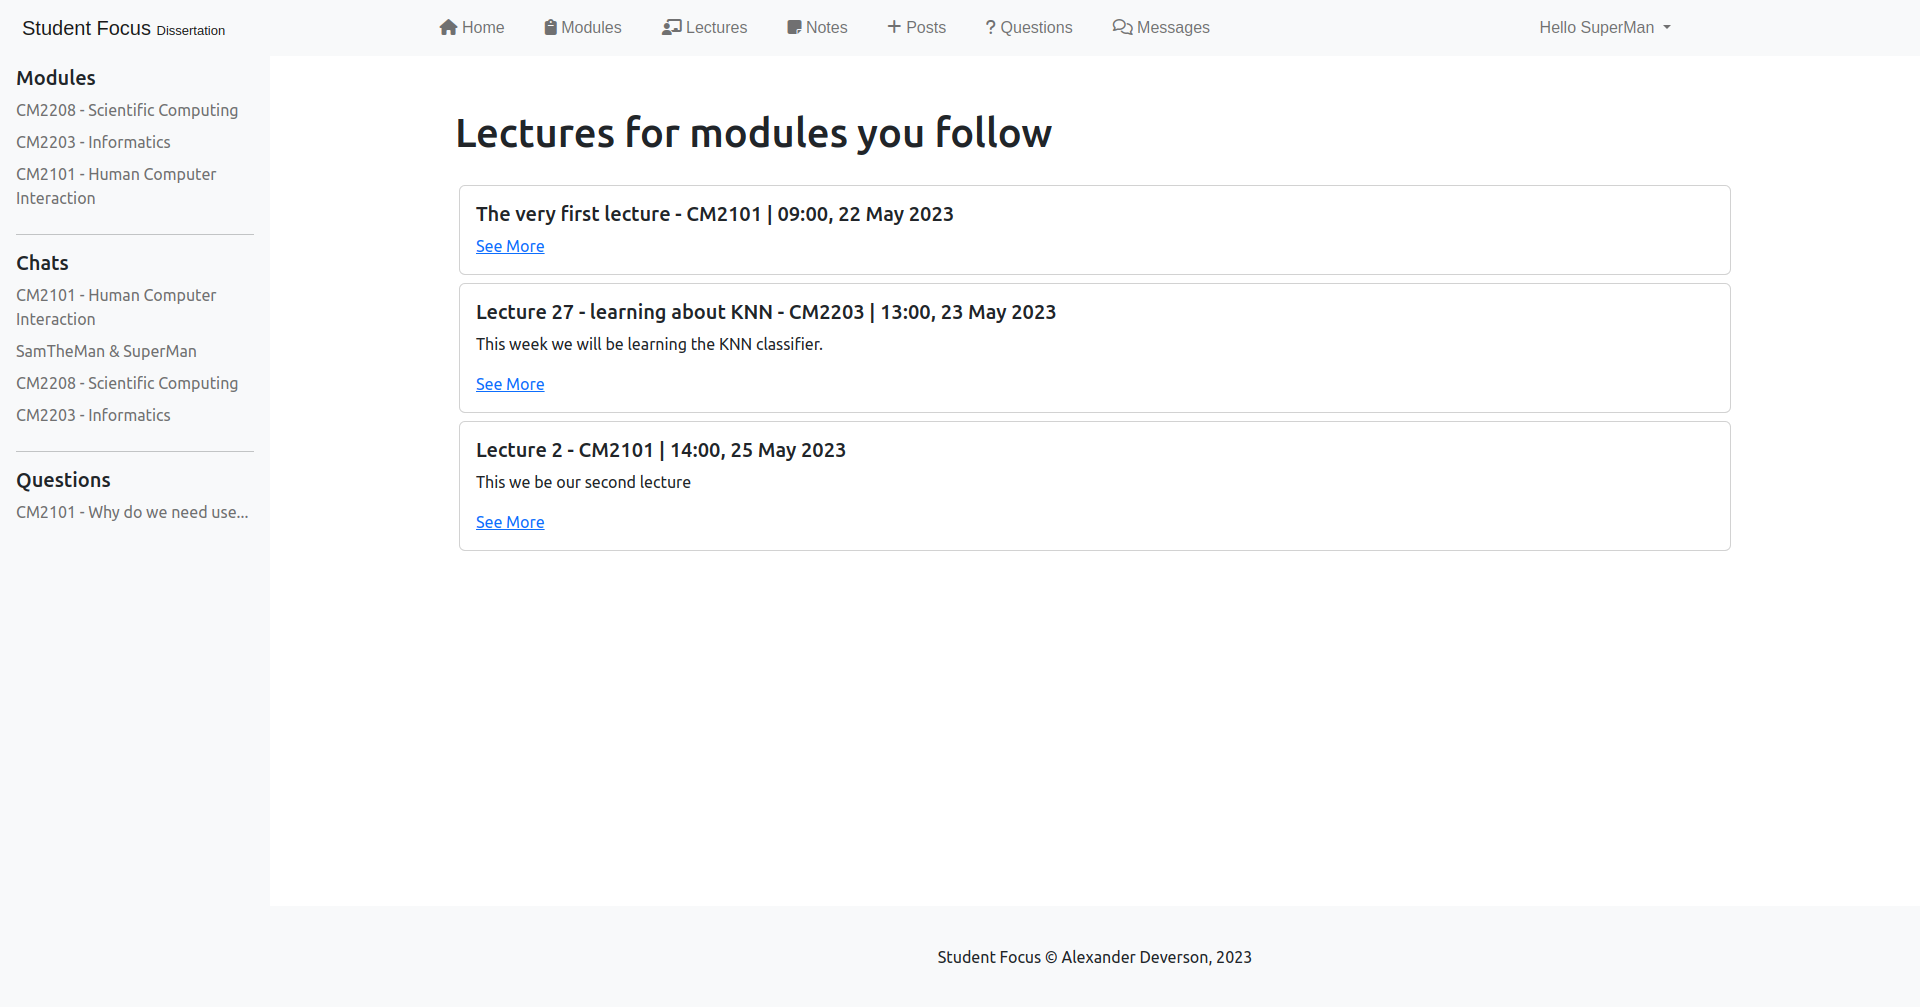
\includegraphics[scale=0.20]{images/application/39 - lecture_list_more.png}

A page listing all the lectures for the modules that a user has subscribed to (but from a user with more modules and desktop version)

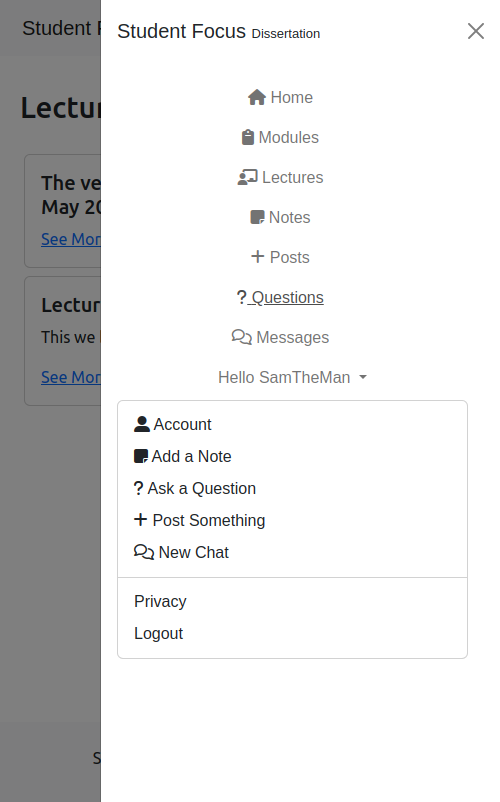
\includegraphics[scale=0.20]{images/application/41 - mobile_menu.png}

The mobile version of the navigation menu

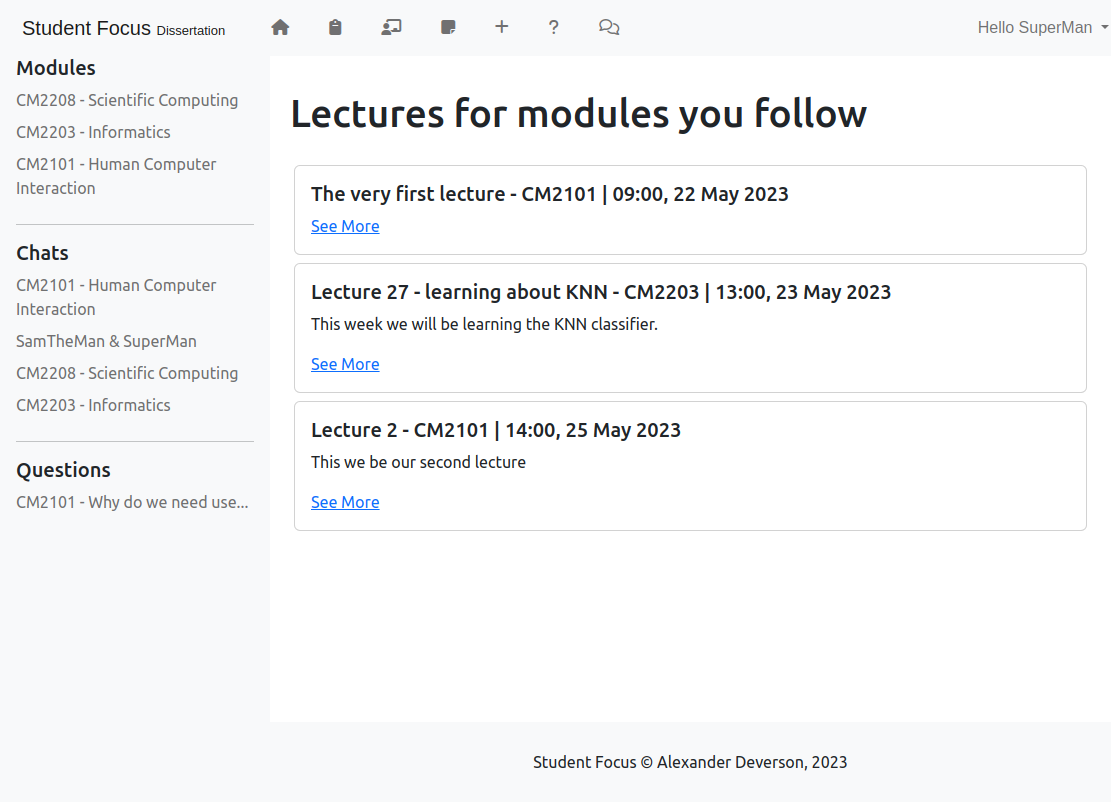
\includegraphics[scale=0.20]{images/application/42 - responsive.png}

Showing the site responsive with the menu icons only

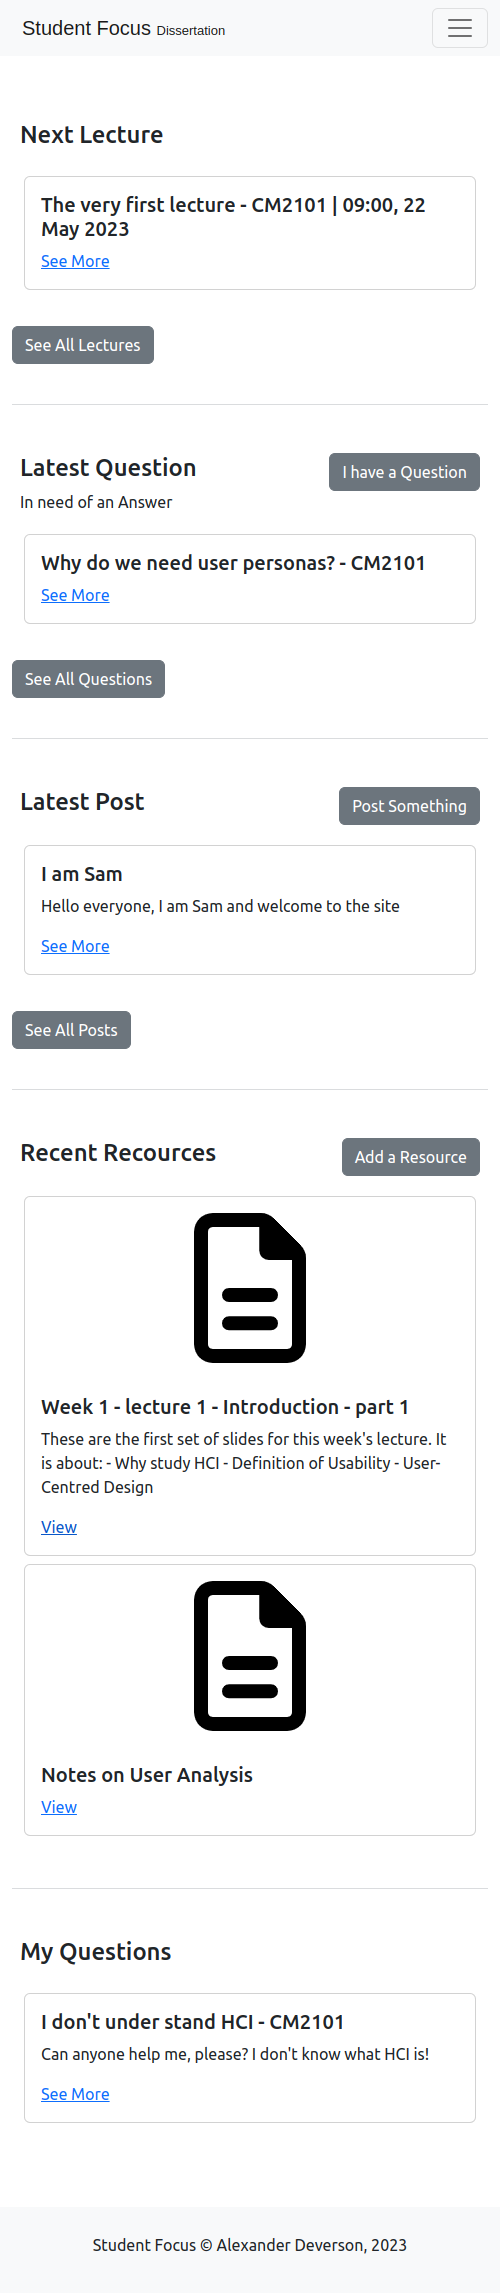
\includegraphics[scale=0.20]{images/application/44 - mobile_home.png}

The mobile version of the user's home page

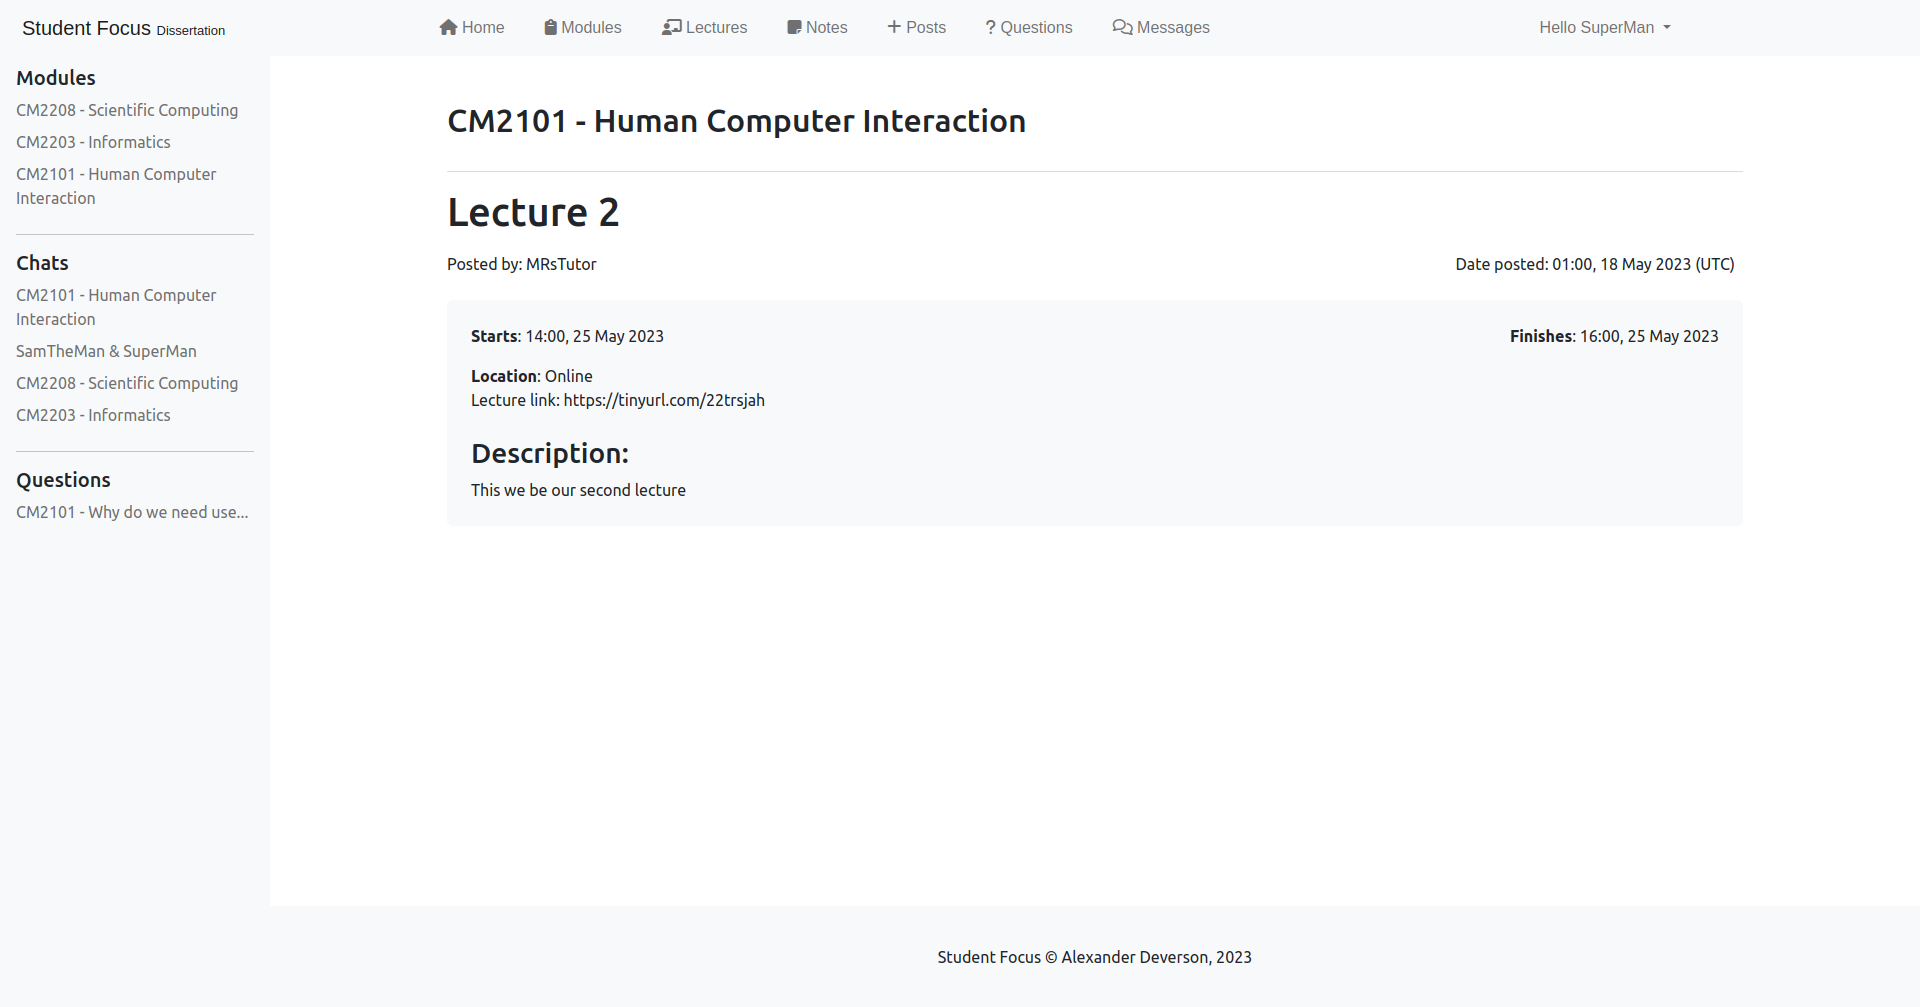
\includegraphics[scale=0.20]{images/application/45 - lecture_single.png}

Single lecture page

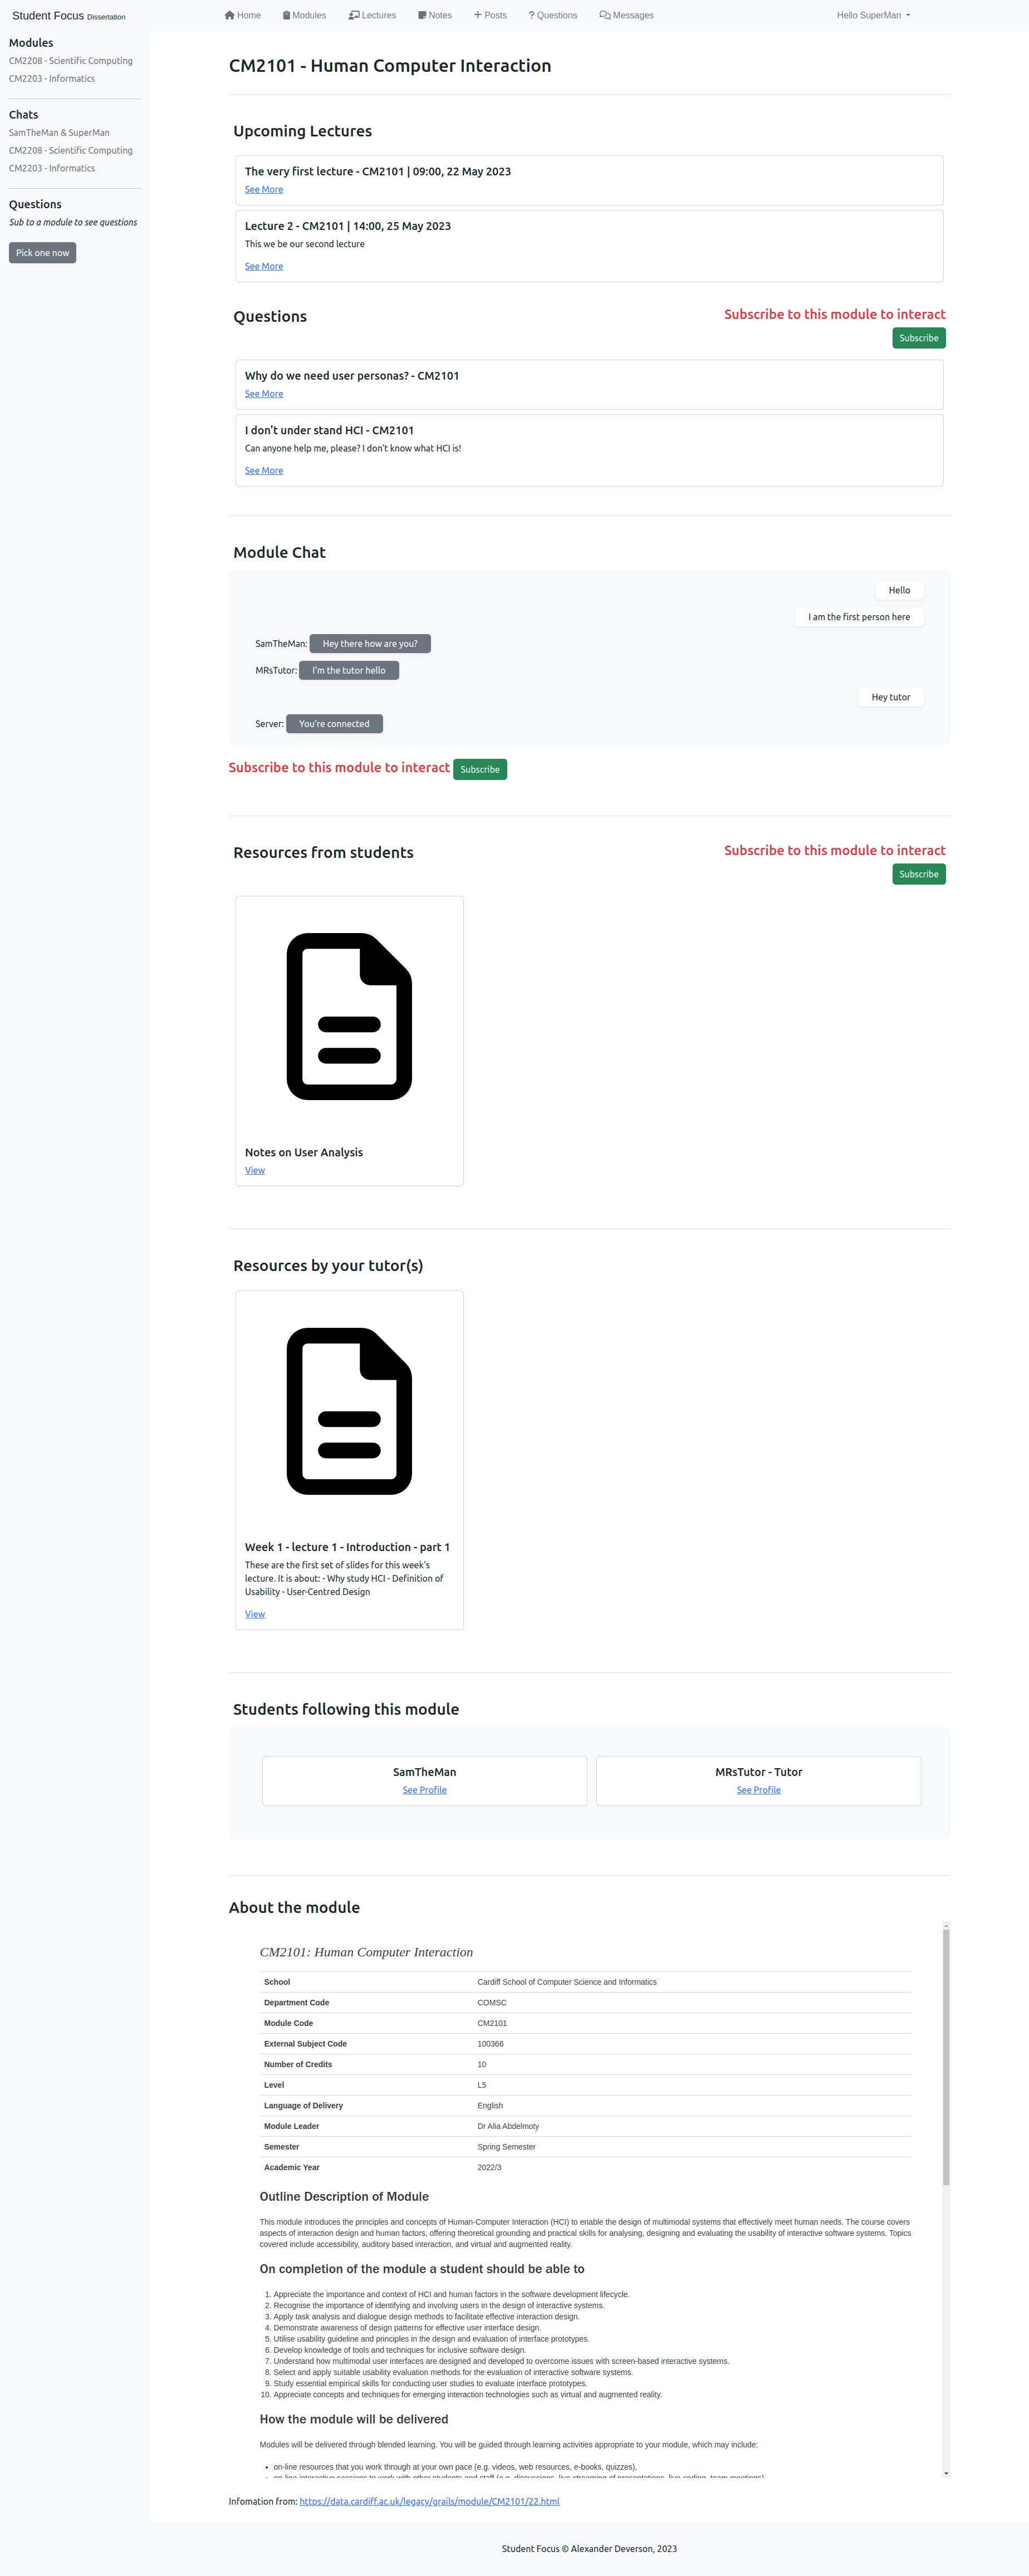
\includegraphics[scale=0.12]{images/application/46 - non_subed_module.png}

single module page showing a user not subscribed to the module

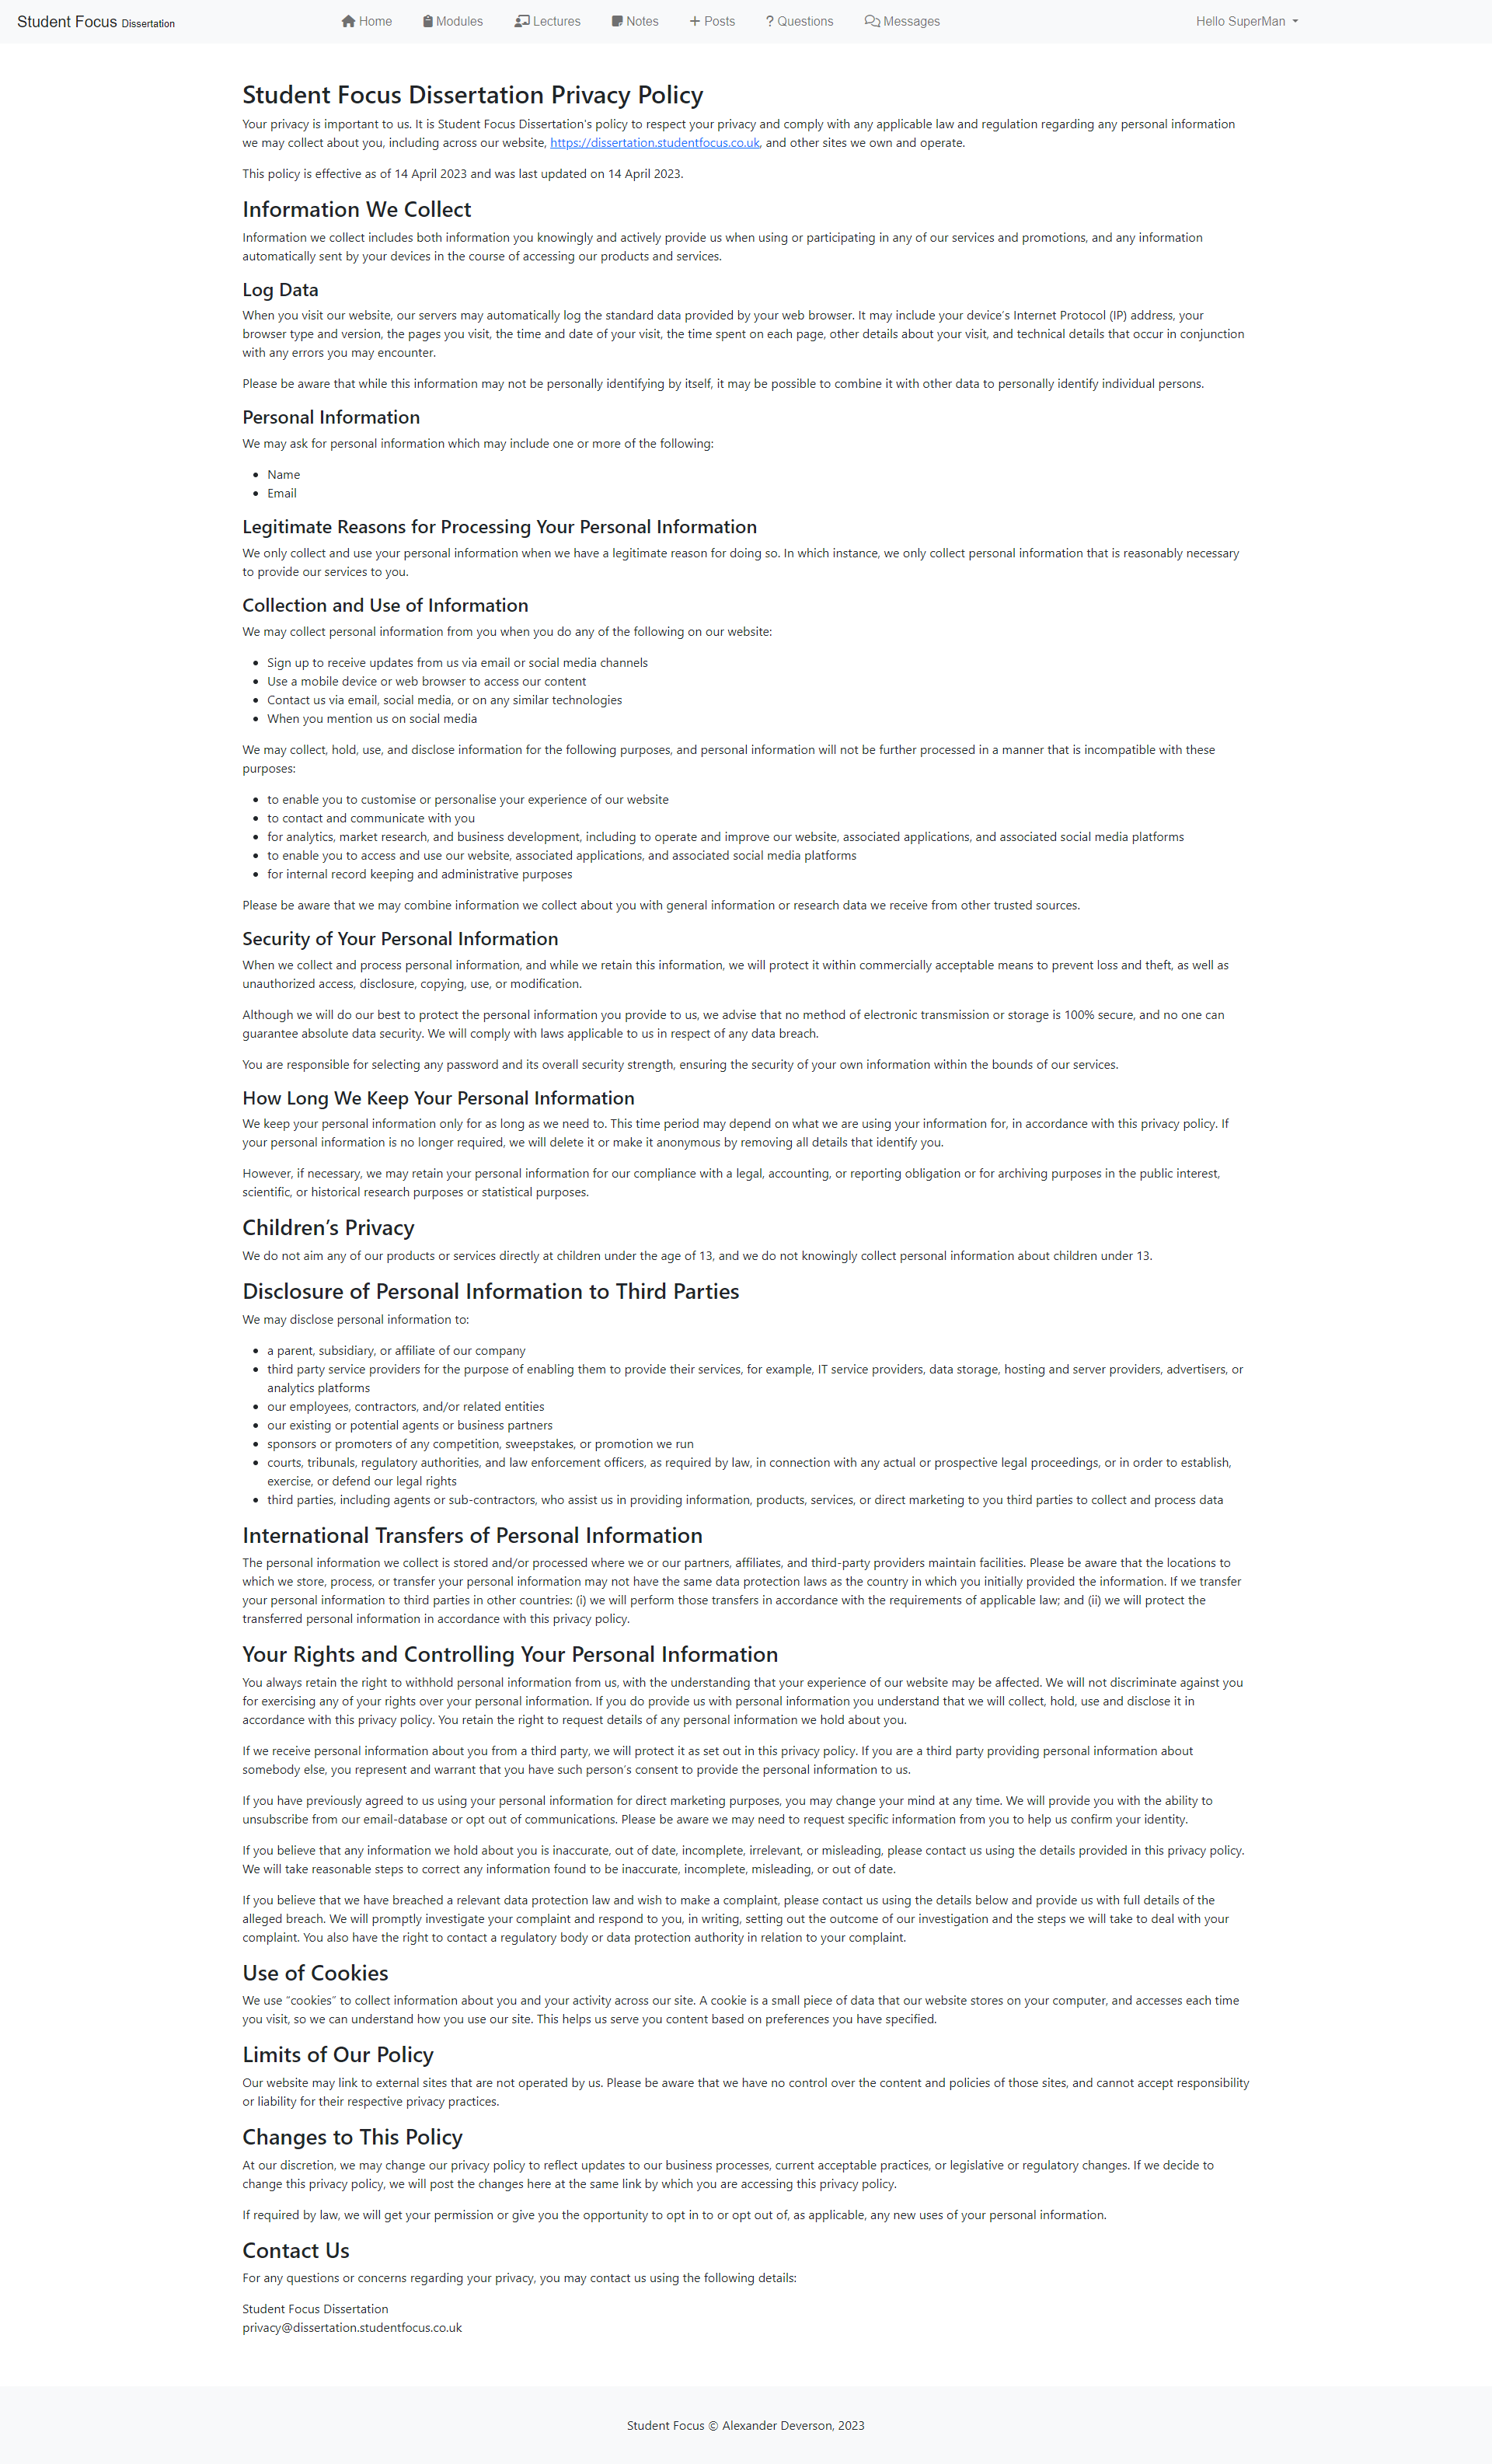
\includegraphics[scale=0.20]{images/application/47 - privacy.png}

The privacy page

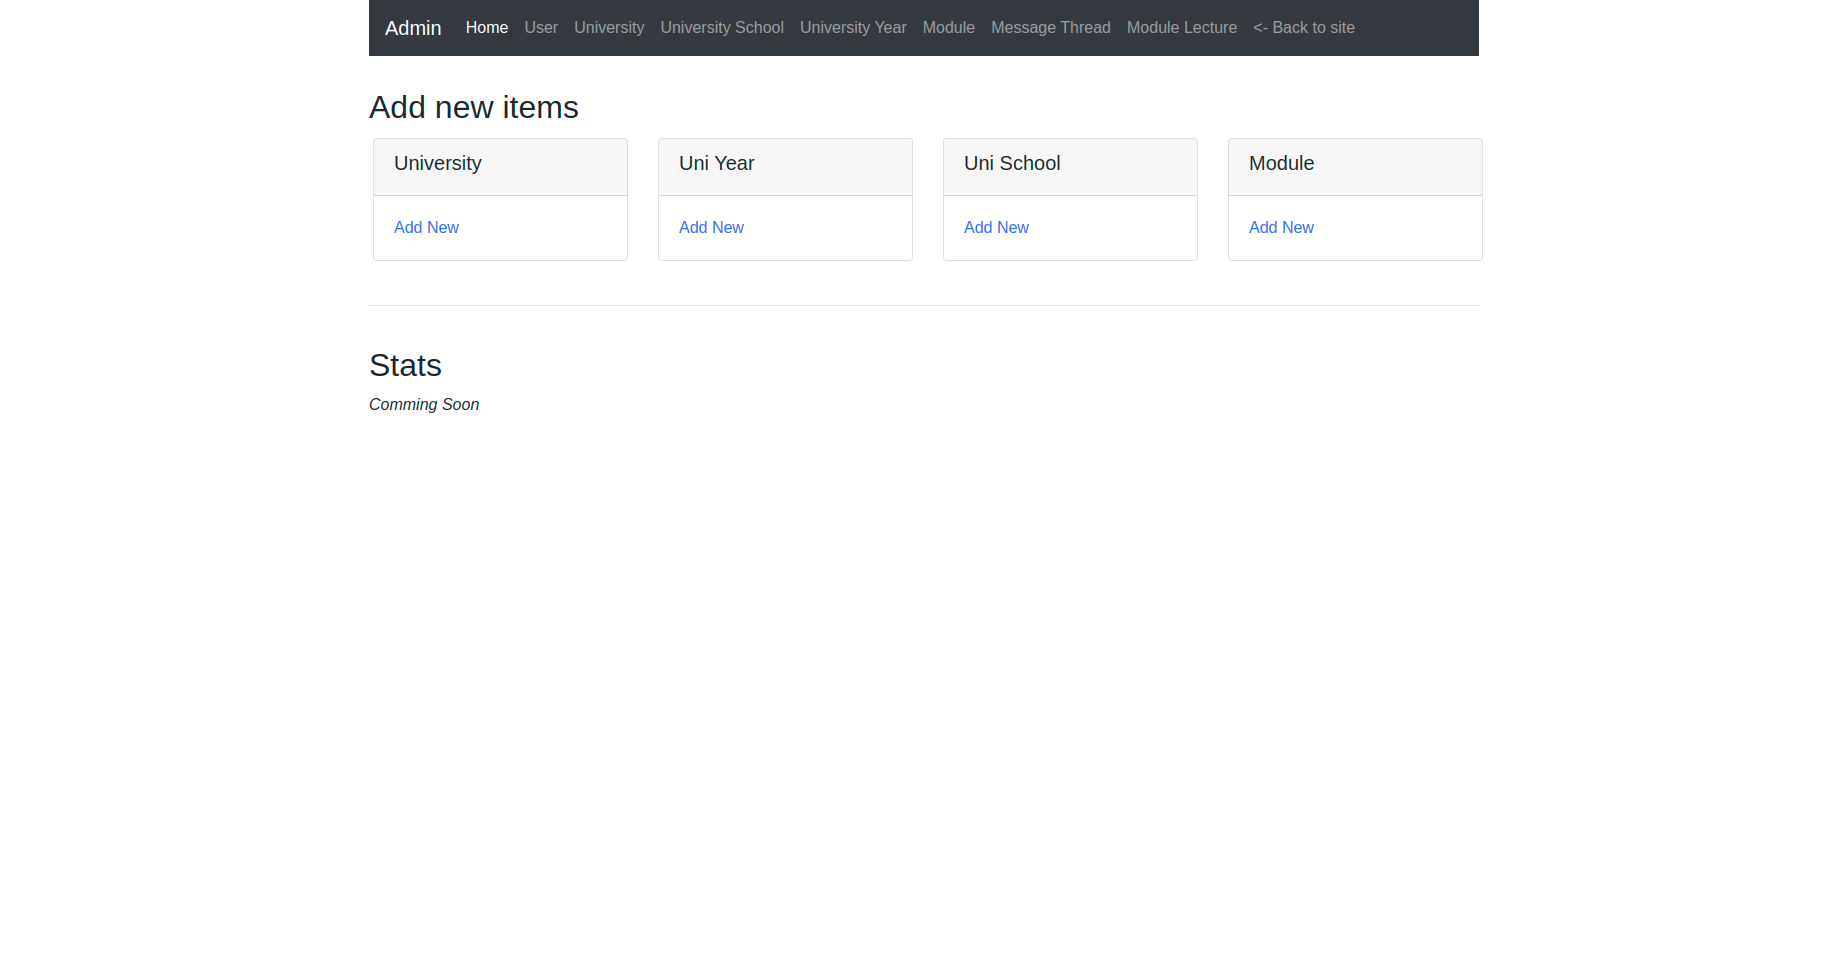
\includegraphics[scale=0.20]{images/application/48 - admin_home.png}

The admin home page

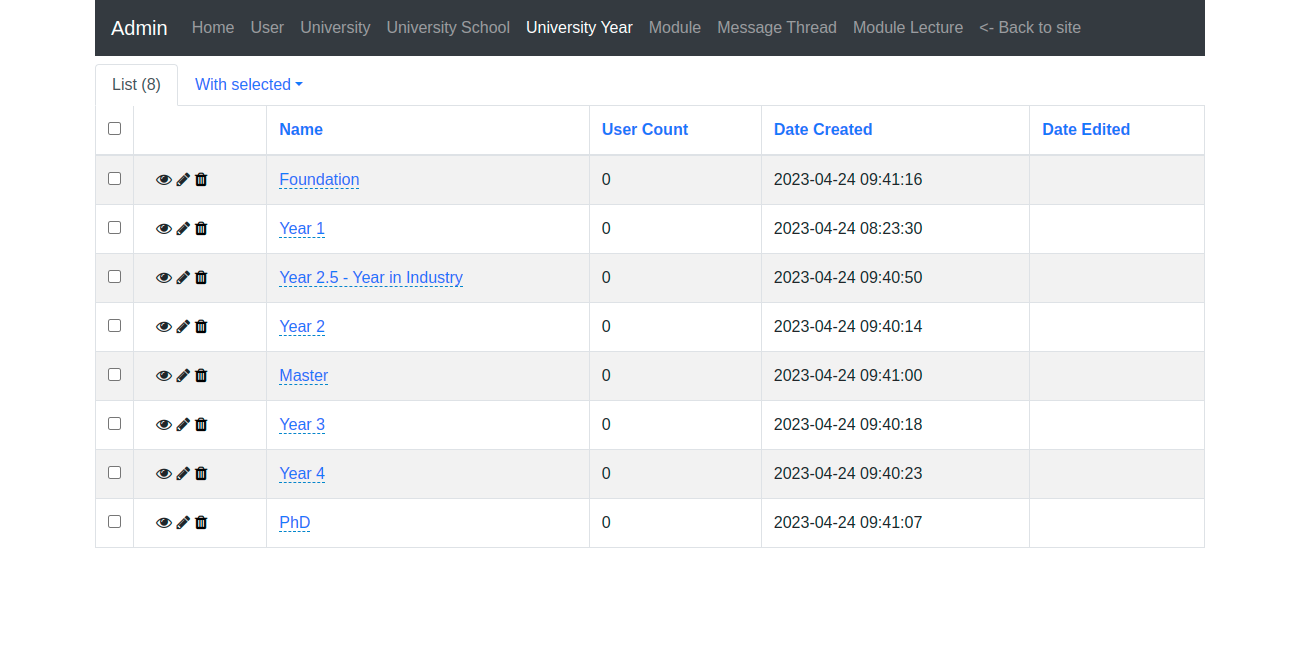
\includegraphics[scale=0.20]{images/application/49 - admin_table_example.png}

An example showing a table that the admin can view from the database

\includegraphics[scale=0.20]{images/application/52 - admin_table_row_single.png}

An example of a row from the table above

\includegraphics[scale=0.20]{images/application/50 - admin_add_uni.png}

The form page for adding a new university to the application. University School and Year look the same.

\includegraphics[scale=0.20]{images/application/51 - admin_add_module.png}

The form page for the admin to add a new module to the application

\includegraphics[scale=0.50]{images/application/55 - nav_user_dropdwon.png}

User navigation dropdown

\includegraphics[scale=0.27]{images/application/56 - student_resource.png}

Student resources of the single module page

\includegraphics[scale=0.27]{images/application/57 - tutor_resource.png}

Tutor resources of the single module page

\includegraphics[scale=0.50]{images/application/58 - nav_hover.png}

When hovering over a page link in the navigation

\includegraphics[scale=0.27]{images/application/59 - message_hover.png}

When hovering over a message in the real-time chat section

\includegraphics[scale=0.50]{images/application/60 - aside_module_hover.png}

When hovering over a module in the sidebar

\includegraphics[scale=0.50]{images/application/61 - aside_chat_hover.png}

When hovering over a message thread in the sidebar

\includegraphics[scale=0.50]{images/application/62 - aside_question_hover.png}

When hovering over a question in the sidebar

\includegraphics[scale=0.27]{images/application/63 - load_more_messages.png}

When needing to load older messages

\includegraphics[scale=0.27]{images/application/64 - lectures.png}

Example showing when there are too many items, such as lectures, questions, posts, comments, etc, and they become paginated





\section{Code snippets}

\subsection{Database design code}
https://mermaid.live was used to for generating the diagrams

\subsubsection{Database - full}

\includegraphics[scale=0.60, angle=90]{images/database/database_diagram.png}

\begin{lstlisting}
erDiagram
    User ||--o{ ModuleSubscription:subs
    ModuleSubscription }o--|| Module:connects
    User ||--o{ Note:owns
    User }o--|| University:belong_to
    User }o--|| UniversitySchool:has
    User }o--|| UniversityYear:has
    User ||--o| ModuleResource:links_to
    User ||--o{ ModuleReview:owns
    
    ModuleReview ||--o{ Module:belongs_to
    UniversityYear ||--o{ Module:belongs_to
    UniversitySchool ||--o{ Module:belongs_to
    University ||--o{ Module:belongs_to

    ModuleQuestion }o--|| Module:has
    Note }o--|| Module:links_to
    User ||--o{ ModuleQuestion:has
    ModuleQuestionComment }o--|| ModuleQuestion:has
    User ||--o{ ModuleQuestionComment:has
    ModuleLecture }o--|| Module:has
    User ||--o{ ModuleLecture:has
    ModuleResource }o--|| Module:has
    MessageThread ||--|| Module:links_to


    PublicPost ||--o{ PublicPostComment:has
    PublicPostComment }o--|| User:has
    PublicPost }o--|| User:has
    PublicProfile ||--|| User:links_to

    User ||--o{ MessageThread:owns
    user_message_thead_link }o--|| User:links_to
    Message }o--|| MessageThread:has
    User ||--o{ Message:has
    user_message_thead_link }o--|| MessageThread:links_to

    User ||--o{ Image:owns
    User ||--o{ Document:owns

    Document ||--o| ModuleResource:links_to
    Image ||--o| ModuleResource:links_to    
\end{lstlisting}

\subsubsection{Database - Module focused}

\includegraphics[scale=0.58, angle=90]{images/database/db_module.png}

\begin{lstlisting}
erDiagram
    ModuleReview }o--|| Module:belongs_to

    Module }o--|| UniversityYear:belongs_to
    Module }o--|| UniversitySchool:belongs_to
    Module }o--|| University:belongs_to
    
    Module ||--o{ModuleLecture:has
    ModuleSubscription }o--|| Module:connects
    ModuleResource }o--|| Module:has


    MessageThread ||--|| Module:links_to

    ModuleQuestion }o--|| Module:has
    ModuleQuestion ||--o{ ModuleQuestionComment:has
    Module ||--o{ Note:links_to


    %% table description

    Module {
        string(20) id PK
        string(240) name
        string(30) code
        float avg_rating
        text description
        string(240) tutor
        datetime date_created
        datetime date_edited
        string(20) university_id PK, FK
        string(20) university_school_id PK, FK
        string(20) university_year_id PK, FK
        string(20) message_thread_id PK, FK
    }

    ModuleSubscription {
        string(20) id PK
        datetime date_added
        string(20) user_id PK, FK
        string(20) module_id PK, FK        
    }

    ModuleQuestion {
        string(20) id PK
        string(240) title
        text description
        datetime date
        datetime date_edited
        int(1) solved
        int comment_count
        int view_count
        int unique_view_count
        string(20) user_id PK, FK
        string(20) module_id PK, FK 
    }

    ModuleQuestionComment {
        string(20) id PK
        datetime date_sent
        datetime date_edited
        text message
        int sub_comment_count
        string(20) user_id PK, FK
        string(20) module_question_id PK, FK
    }

    ModuleResource {
        string(20) id PK
        datetime date
        int(1) is_tutor_resource
        string(20) user_id PK, FK
        string(20) module_id PK, FK
        string(20) image_id PK, FK
        string(20) document_id PK, FK
    }

    ModuleLecture {
        string(20) id PK
        string(100) title
        datetime date_added
        datetime date_start
        datetime date_end
        string(100) location
        text description
        string(300) online_link
        string(300) quizing_link
        string(20) module_id PK, FK
        string(20) user_id PK, FK
    }

    UniversityYear {
        string(20) id PK
        string(120) name
        int user_count
        datetime date_created
        datetime date_edited
    }

    UniversitySchool {
        string(20) id PK
        string(120) name
        int user_count
        datetime date_created
        datetime date_edited
    }

    University {
        string(20) id PK
        string(120) name
        string(300) url
        datetime date_created
        datetime date_edited
        datetime date_established
        string(120) first_line
        string(120) second_line
        string(100) city
        string(100) country
        string(20) postcode
        int user_count
        float avg_rating
    }

    Note {
        string(20) id PK
        datetime date_created
        datetime date_edited
        string title
        text text
        string user_id PK, FK
        string module_id PK, FK
    }

    MessageThread {
        string(20) id PK
        string(240) name
        datetime date
        datetime date_last_message
        int member_count
        int message_count
        string(20) user_id PK, FK
    }

    ModuleReview {
        string(20) id PK
        string(240) title
        int rating
        text description
        datetime date_sent
        datetime date_edited
        string(20) user_id PK, FK
        string(20) module_id PK, FK
    }
\end{lstlisting}

\subsubsection{Database - User focused}

\includegraphics[scale=0.55, angle=90]{images/database/db_user.png}

\begin{lstlisting}
erDiagram 
    User ||--|| PublicProfile:links_to

    User ||--o{ ModuleSubscription:subs
    User ||--o{ Note:owns
    User }o--|| University:belong_to
    User }o--|| UniversitySchool:has
    User }o--|| UniversityYear:has
    User }o--|| ModuleReview:has

    ModuleQuestionComment }o--|| User:has
    ModuleQuestion ||--o{ ModuleQuestionComment:has
    ModuleQuestion ||--o{ User:has
    User ||--o{ ModuleLecture:has
    ModuleResource |o--|| Document:links_to
    ModuleResource |o--|| Image:links_to

    Document }o--|| User:owns
    ModuleResource }o--|| User:has
    Image }o--|| User:owns

    MessageThread }o--|| User:owns
    Message }o--|| User:has
    user_message_thread_link }o--|| User:links_to
    PublicPostComment }o--|| User:has
    
    PublicPost }o--|| User:has
    PublicPostComment }o--|| PublicPost:has
    MessageThread ||--o{ Message:has
    user_message_thread_link }o--|| MessageThread:links_to


    %% table description

    User {
        string(20) id PK
        string(120) username
        string(120) firstname
        string(120) lastname
        string(120) email
        string(128) password
        datetime join_date
        int(1) is_admin
        int(1) is_tutor
        string(20) university_id PK, FK
        string(20) university_year_id PK, FK
        string(20) university_school_id PK, FK
        string(20) public_profile_id PK, FK
    }
\end{lstlisting}

\subsubsection{Database - Social focused}

\includegraphics[scale=0.58, angle=90]{images/database/db_social.png}

\begin{lstlisting}
erDiagram
    PublicPostComment }o--|| User:has
    PublicPost }o--|| User:has
    PublicPost ||--o{ PublicPostComment:has
    
    PublicProfile ||--|| User:links_to

    MessageThread }o--|| User:owns
    Message }o--|| User:has

    Message }o--|| MessageThread:has
    
    user_message_thread_link }o--|| MessageThread:links_to

    user_message_thread_link }o--|| User:links_to
    Module ||--|| MessageThread:links_to


    %% table description

    MessageThread {
        string(20) id PK
        string(240) name
        datetime date
        datetime date_last_message
        int member_count
        int message_count
        string(20) user_id PK, FK
    }

    Message {
        string(20) id PK
        text body
        datetime date_sent
        datetime date_edited
        string(20) user_id PK, FK
        string(20) message_thread_id PK, FK
    }

    user_message_thread_link {
        string(20) user_id PK, FK
        string(20) message_thread_id PK, FK
    }

    User {
        string(20) id PK
        string(120) username
        string(120) firstname
        string(120) lastname
        string(120) email
        string(128) password
        datetime join_date
        int(1) is_admin
        int(1) is_tutor
        string(20) university_id PK, FK
        string(20) university_year_id PK, FK
        string(20) university_school_id PK, FK
        string(20) public_profile_id PK, FK
    }

    PublicProfile {
        %% # Datebase Columns 
        string(20) id PK
        text bio
        datetime date_edited
    }

    PublicPost {
        string(20) id PK
        string(240) title
        text description
        datetime date
        datetime date_edited
        int comment_count
        int view_count
        int unique_view_count
        string(20) user_id PK, FK
        string(20) university_id PK, FK
        string(20) university_school_id PK, FK
        string(20) university_year_id PK, FK
    }

    PublicPostComment {
        string(20) id PK
        datetime date
        datetime date_edited
        text message
        int sub_comment_count
        string(20) user_id PK, FK
        string(20) public_post_id PK, FK
        string(20) parent_comment_id PK, FK
    }
\end{lstlisting}

\subsubsection{Database - Module Resource focused}

\includegraphics[scale=0.63]{images/database/db_module_resource.png}

\begin{lstlisting}
erDiagram
    ModuleResource }o--|| Module:has
    User ||--o{ Document:owns
    ModuleResource |o--|| Document:links_to
    User ||--o{ ModuleResource:has
    ModuleResource |o--|| Image:links_to
    User ||--o{ Image:owns


    %% table description

    Module {
        string(20) id PK
        string(240) name
        string(30) code
        float avg_rating
        text description
        string(240) tutor
        datetime date_created
        datetime date_edited
        string(20) university_id PK, FK
        string(20) university_school_id PK, FK
        string(20) university_year_id PK, FK
        string(20) message_thread_id PK, FK
    }

    ModuleResource {
        string(20) id PK
        datetime date
        int(1) is_tutor_resource
        string(20) user_id PK, FK
        string(20) module_id PK, FK
        string(20) image_id PK, FK
        string(20) document_id PK, FK
    }

    Document {
        string(20) id PK
        string(240) title
        text description
        datetime date
        string(300) imagekit_id
        string(20) file_type
        string(20) user_id PK, FK
    }

    Image {
        string(20) id PK
        string(240) title
        text description
        datetime date
        string(300) imagekit_id
        string(20) file_type
        string(20) user_id PK, FK
    }

    User {
        string(20) id PK
        string(120) username
        string(120) firstname
        string(120) lastname
        string(120) email
        string(128) password
        datetime join_date
        int(1) is_admin
        int(1) is_tutor
        string(20) university_id PK, FK
        string(20) university_year_id PK, FK
        string(20) university_school_id PK, FK
        string(20) public_profile_id PK, FK
    }
\end{lstlisting}

\subsection{System diagram}

\includegraphics[scale=0.63]{images/System_Architecture_Diagram.jpeg}

\section{Chat GTP}

\section{Future user survey}
\begin{enumerate}
    \item What school are you part of? (ie COMSC, Business, Engineering, etc)
    \begin{itemize}
	\item (Text box)
    \end{itemize}
    
    \item What VLEs (Virtual Learning Environments) have you used in the past? (multi-select)
    \begin{itemize}
        \item Blackboard Learn (Learning Central)
        \item Google classroom
        \item Moodle
	\item D2L Brightspace
        \item Schoology
        \item Cornerstone Learning
        \item Docebo
        \item Litmos
        \item TalentLMS
    \end{itemize}
    
    \item What resources do you use for university? (multi-select)
    \begin{itemize}
        \item Learning Central
        \item Teams
        \item Panopto
        \item Zoom
        \item Blackboard call
        \item Youtube
        \item Books
        \item Student app
        \item Discord
        \item Yammer
        \item Menti meter
        \item Kahoot
        \item Zotero 
        \item Add others (Text box) 
    \end{itemize}
    
    \item How often do you typically use Learning Central?
    \begin{itemize}
        \item Not often
        \item Once per week
        \item Multi times a week (2-4)
        \item Once Ever day
        \item Multi times a day
    \end{itemize}
    
    \item How often do you typically use MS Teams?
    \begin{itemize}
        \item Not often
        \item Once per week
        \item Multi times a week (2-4)
        \item Once Ever day
        \item Multi times a day 
    \end{itemize}
    
    \item How often do you typically use Emails?
    \begin{itemize}
        \item Not often
        \item Once per week
        \item Multi times a week (2-4)
        \item Once Ever day
        \item Multi times a day 
    \end{itemize}
    
    \item How do you prefer to learn?
    \begin{itemize}
        \item Online – videos
        \item Online - books/slides
        \item Practical Labs
        \item In-person
        \item A mixture 
    \end{itemize}
    
    \item Do you find value in lectures being recorded? (In-person and online video calls)
    \begin{itemize}
        \item Yes, I like to watch them back later
        \item No. I take good notes
        \item Doesn't matter, I don't learn from the lectures
    \end{itemize}
    
    \item Do you have a group for everyone in your Year on the course?
    \begin{itemize}
        \item We have a big group to discussion(s)
        \item Only between a few friends/class mates
        \item No I only talk to people on my course when I have too
        \item What the tutors provide are good enough 
    \end{itemize}
    
    \item Do you find it easy to locate resources and navigate course content?
    \begin{itemize}
        \item My tutors organise content so it's easy to locate 
        \item Things feel messy and unorganised
        \item No, resources are spread across too many locations/apps 
    \end{itemize}
    
    \item Is course content uploaded in a consistent way across all your modules?
    \begin{itemize}
        \item Mostly
        \item Somewhat consistent 
        \item Every module is different 
        \item Definitely not; tutors in the same module do things their own way
    \end{itemize}
    
    \item Would you find it easier to have course content, your timetable and connecting \& discussing topics in one website?
    \begin{itemize}
        \item Yes
        \item No
        \item Doesn't bother me, what we have works good enough 
    \end{itemize}
    
    \item Do you use Discord for uni?
    \begin{itemize}
        \item Yes, my class has a server for us to discuss the Modules
        \item No, only for personal/gaming 
        \item No Discord is too complicated/I'm not sure how to use it 
    \end{itemize}
    
    \item Where are most of your Module resources located?
    \begin{itemize}
        \item Most of my tutors use teams
        \item Most of my tutors use LC
        \item They use a mixture of the two
        \item Most of my tutors use something different (optional text box)
        \item Most of my content is only inperson/paper hand outs 
    \end{itemize}
    
    \item Do you take notes?
    \begin{itemize}
        \item I don't take notes 
        \item Yes 
    \end{itemize}
    
    \item Do you take notes?
    \begin{itemize}
        \item I don't take notes 
        \item Yes 
    \end{itemize}
    
    \item How do you take notes? (multi select)
    \begin{itemize}
        \item On paper
        \item On panopto videos
        \item Word/text editor
        \item An app like onenote/obsidian/notion
        \item Discord or other social media sites
        \item Text myself
    \end{itemize}
    
    \item Do you share note with friends/class mates?
    \begin{itemize}
        \item No they're my notes
        \item No but I wouldn't have a problem with sharing 
        \item When some misses a lecture 
        \item We often exchange notes to help eachother  
    \end{itemize}
    
    \item \textbf{}
    \begin{itemize}
        \item Only when I have too
        \item Never, it feels too formal and intimating
        \item Sometimes
        \item Often, I'm forever messaging tutors with questions
        \item No I use teams instead
        \item No I use discussions on LC instead 
    \end{itemize}
    
    \item Do you dislike anything about the current VLE (LC)?
    \begin{itemize}
        \item (Text box) 
    \end{itemize}
    
    \item If you could added/change anything about the current VLE (LC), what would it be?
    \begin{itemize}
        \item (Text box) 
    \end{itemize}
    
    \item Is there something that you believe the current system does really well?
    \begin{itemize}
        \item (Text box) 
    \end{itemize}
\end{enumerate}